\documentclass[11pt]{article}

\usepackage[a4paper,margin=23mm,includeheadfoot,headheight=15pt,headsep=15pt,footskip=22pt]{geometry}
\usepackage[nopatch=footnote]{microtype}
\usepackage{amsmath,amssymb,amsthm,mathtools}
\usepackage{aliascnt}
\usepackage{booktabs,longtable,array,tabularx}
\usepackage{enumitem}
\usepackage{fancyhdr}
\PassOptionsToPackage{hyphens}{url}
\usepackage{hyperref}
\usepackage[nameinlink,noabbrev]{cleveref}
\usepackage[table]{xcolor}
\usepackage{setspace}
\usepackage[most]{tcolorbox}
\usepackage{needspace}
\usepackage{multicol}
\usepackage{makecell}
\usepackage{graphicx,tikz,titlesec,bookmark,caption,etoolbox,tocloft}
\setlength{\cftbeforesecskip}{4pt}
\usetikzlibrary{arrows.meta,decorations.pathreplacing,patterns,calc}
\graphicspath{{figures/}}
\definecolor{accent}{HTML}{137668}\definecolor{muted}{HTML}{536568}
\frenchspacing\emergencystretch=2em\clubpenalty=10000\widowpenalty=10000\raggedbottom
\titleformat{\section}{\sffamily\bfseries\large\color{accent}}{\thesection}{.7em}{}
\titleformat{\subsection}{\sffamily\bfseries\normalsize}{\thesubsection}{.7em}{}
\titlespacing*{\section}{0pt}{1.4\baselineskip}{.55\baselineskip}
\captionsetup{font=small,labelfont={sf,bf},labelsep=period}
\pretocmd{\section}{\Needspace{7\baselineskip}}{}{}
\pretocmd{\subsection}{\Needspace{5\baselineskip}}{}{}
\newcolumntype{L}[1]{>{\raggedright\arraybackslash}p{#1}}
\newcommand{\cA}{\mathcal A}\newcommand{\cB}{\mathcal B}\newcommand{\cP}{\mathcal P}
\newcommand{\R}{\mathbb R}\newcommand{\C}{\mathbb C}\newcommand{\Z}{\mathbb Z}\newcommand{\N}{\mathbb N}
\newcommand{\Spec}{\operatorname{Spec}}\newcommand{\rank}{\operatorname{rank}}\newcommand{\diag}{\operatorname{diag}}
\newcommand{\closure}[1]{\overline{#1}}


\allowdisplaybreaks
\setstretch{1.055}
\setlength{\parskip}{0.30em}
\setlength{\parindent}{1.35em}
\setlist[itemize]{topsep=0.35em,itemsep=0.15em,leftmargin=1.6em}
\setlist[enumerate]{topsep=0.35em,itemsep=0.15em,leftmargin=1.8em}
\definecolor{PSCBlue}{RGB}{44,83,118}
\definecolor{PSCLightBlue}{RGB}{242,247,251}
\definecolor{PSCGreen}{RGB}{49,105,83}
\definecolor{PSCLightGreen}{RGB}{243,249,246}
\definecolor{PSCAmber}{RGB}{132,91,21}
\definecolor{PSCLightAmber}{RGB}{252,248,238}
\definecolor{PSCGray}{RGB}{90,96,102}
\definecolor{PSCLightGray}{RGB}{247,247,247}

\newtcolorbox{readerroadmap}[1][]{
  enhanced,breakable,colback=PSCLightBlue,colframe=PSCBlue,
  boxrule=0.65pt,arc=1.2mm,left=1.4mm,right=1.4mm,top=1mm,bottom=1mm,
  fonttitle=\bfseries,title={Reader roadmap},#1}
\newtcolorbox{keyidea}[1][]{
  enhanced,breakable,colback=PSCLightGreen,colframe=PSCGreen,
  boxrule=0.65pt,arc=1.2mm,left=1.4mm,right=1.4mm,top=1mm,bottom=1mm,
  fonttitle=\bfseries,title={Key idea},#1}
\newtcolorbox{interpretation}[1][]{
  enhanced,breakable,colback=PSCLightGray,colframe=PSCGray,
  boxrule=0.55pt,arc=1.2mm,left=1.4mm,right=1.4mm,top=1mm,bottom=1mm,
  fonttitle=\bfseries,title={Interpretation},#1}
\newtcolorbox{microexample}[1][]{
  enhanced,breakable,colback=PSCLightAmber,colframe=PSCAmber,
  boxrule=0.55pt,arc=1.2mm,left=1.4mm,right=1.4mm,top=1mm,bottom=1mm,
  fonttitle=\bfseries,title={Running example},#1}
\newtcolorbox{hypothesisguide}[1][]{
  enhanced,breakable,colback=white,colframe=black!45,
  boxrule=0.5pt,arc=1.2mm,left=1.4mm,right=1.4mm,top=1mm,bottom=1mm,
  fonttitle=\bfseries,title={Why the hypotheses matter},#1}
\newtcolorbox{sectionrecap}[1][]{
  enhanced,breakable,colback=white,colframe=PSCBlue,
  borderline west={2pt}{0pt}{PSCBlue},boxrule=0pt,arc=0mm,
  left=2mm,right=1mm,top=0.8mm,bottom=0.8mm,
  fonttitle=\bfseries,title={Section recap},#1}
\newtcolorbox{warningbox}[1][]{
  enhanced,breakable,colback=PSCLightAmber,colframe=PSCAmber,
  boxrule=0.65pt,arc=1.2mm,left=1.4mm,right=1.4mm,top=1mm,bottom=1mm,
  fonttitle=\bfseries,title={Do not conflate},#1}
\newcommand{\ProofMap}[1]{\begin{interpretation}[title={Proof map}]#1\end{interpretation}}
\newcommand{\ConceptChain}[1]{\begin{center}\fbox{\begin{minipage}{0.92\textwidth}\centering #1\end{minipage}}\end{center}}

\hypersetup{
  pdftitle={Projector Resolved Seed Calculus I: Typed Operator Systems, Seed Rank, and Exact Packet Coordinates},
  pdfauthor={Komorebi P.},
  pdfsubject={Expanded symbolic and expository foundation},
  colorlinks=true,
  linkcolor=black,
  citecolor=black,
  urlcolor=black
}

\pagestyle{fancy}
\fancyhf{}
\fancyhead[L]{\sffamily\fontsize{8}{10}\selectfont\color{muted}KOMOREBI MATHEMATICS / PAPER I}
\fancyhead[R]{\sffamily\fontsize{8}{10}\selectfont\color{muted}TRADITIONAL PAPER}
\fancyfoot[L]{\sffamily\fontsize{8}{10}\selectfont\color{muted}Projector-resolved seed calculus}\fancyfoot[R]{\sffamily\small\color{accent}\thepage}
\setlength{\headheight}{14pt}

\newtheorem{theorem}{Theorem}[section]
\newaliascnt{proposition}{theorem}
\newtheorem{proposition}[proposition]{Proposition}
\aliascntresetthe{proposition}
\newaliascnt{lemma}{theorem}
\newtheorem{lemma}[lemma]{Lemma}
\aliascntresetthe{lemma}
\newaliascnt{corollary}{theorem}
\newtheorem{corollary}[corollary]{Corollary}
\aliascntresetthe{corollary}
\theoremstyle{definition}
\newaliascnt{definition}{theorem}
\newtheorem{definition}[definition]{Definition}
\aliascntresetthe{definition}
\newaliascnt{classicalinput}{theorem}
\newtheorem{classicalinput}[classicalinput]{Classical Input}
\aliascntresetthe{classicalinput}
\theoremstyle{remark}
\newaliascnt{boundary}{theorem}
\newtheorem{boundary}[boundary]{Boundary}
\aliascntresetthe{boundary}
\newaliascnt{remark}{theorem}
\newtheorem{remark}[remark]{Remark}
\aliascntresetthe{remark}

\theoremstyle{definition}\newtheorem{example}[theorem]{Example}
\newtheorem{construction}[theorem]{Construction}
\crefname{theorem}{theorem}{theorems}
\crefname{proposition}{proposition}{propositions}
\crefname{lemma}{lemma}{lemmas}
\crefname{corollary}{corollary}{corollaries}
\crefname{definition}{definition}{definitions}
\crefname{classicalinput}{classical input}{classical inputs}
\crefname{boundary}{boundary}{boundaries}
\crefname{remark}{remark}{remarks}

\newcommand{\bbk}{\Bbbk}
\newcommand{\A}{\mathcal A}
\newcommand{\B}{\mathcal B}
\newcommand{\Ccal}{\mathcal C}
\newcommand{\Pcal}{\mathcal P}
\newcommand{\Qcal}{\mathcal Q}
\newcommand{\Rcal}{\mathcal R}
\newcommand{\Scal}{\mathcal S}
\newcommand{\Hull}{\operatorname{Hull}}
\newcommand{\srank}{\operatorname{srank}}
\newcommand{\psrank}{\operatorname{psrank}}
\newcommand{\End}{\operatorname{End}}
\newcommand{\Hom}{\operatorname{Hom}}
\newcommand{\im}{\operatorname{im}}
\newcommand{\Ker}{\operatorname{Ker}}
\newcommand{\Jac}{\operatorname{Jac}}
\newcommand{\Irr}{\operatorname{Irr}}
\newcommand{\Span}{\operatorname{span}}
\newcommand{\alg}{\operatorname{alg}}
\newcommand{\Reach}{\operatorname{Reach}}
\newcommand{\Supp}{\operatorname{Supp}}
\newcommand{\id}{\mathrm{id}}
\newcommand{\cl}[1]{\overline{#1}}
\newcommand{\RecordID}[1]{\label{record:#1}}
\newcommand{\Depends}[1]{}
\newcommand{\Exports}[1]{}
\newcommand{\BoundaryNote}[1]{\par\noindent\begingroup\footnotesize\color{PSCGray}\raggedright\textbf{Boundary.} #1\par\endgroup}
\newcolumntype{Y}{>{\raggedright\arraybackslash}X}


\newcommand{\OO}{\mathcal O}\newcommand{\FF}{\mathbb F}\newcommand{\QQ}{\mathbb Q}\newcommand{\ZZ}{\mathbb Z}\newcommand{\RR}{\mathbb R}\newcommand{\CC}{\mathbb C}\newcommand{\kk}{\Bbbk}
\renewcommand{\AA}{\mathcal A}\newcommand{\BB}{\mathcal B}
\newcommand{\Fitt}{\operatorname{Fitt}}\newcommand{\Ann}{\operatorname{Ann}}\newcommand{\coker}{\operatorname{coker}}\newcommand{\Tr}{\operatorname{Tr}}
\newcommand{\whot}{\mathbin{\widehat\otimes}}\newcommand{\m}{\mathfrak m}\newcommand{\p}{\mathfrak p}
\newcommand{\head}[1]{\par\vspace{2pt}{\sffamily\bfseries\normalsize #1}\par\vspace{1pt}}
\newcommand{\atlasCaption}[1]{\par\noindent{\footnotesize\color{black!70}#1\par}}
\newtcolorbox{insight}{colback=black!3,colframe=accent,boxrule=0pt,leftrule=1.1pt,arc=0pt,left=10pt,right=10pt,top=3pt,bottom=3pt,before skip=4pt,after skip=4pt,fontupper=\fontsize{9.7}{11.2}\selectfont}
\newcommand{\takeaway}[1]{\begin{insight}\textbf{Read this as:}\ #1\end{insight}}
\newcommand{\vfig}[2][.92]{\par\begingroup\centering\setlength{\dimen0}{#1\linewidth}\resizebox{.90\dimen0}{!}{\input{visual_graphics/#2.tex}}\par\endgroup\vspace{2pt}}
\newcommand{\vpage}[4]{\clearpage\hypertarget{visual:#1}{}\pdfbookmark[2]{V#1. #2}{PIA.visual#1}{\sffamily\small\bfseries\color{accent}PLATE #1 / #3\par}\vspace{5pt}{\sffamily\bfseries\fontsize{22}{25}\selectfont #2\par}\vspace{5pt}{\sffamily\fontsize{8.7}{11}\selectfont\color{black!65}#4\par}\vspace{6pt}}
\newcommand{\pagerefV}[1]{\hyperlink{visual:#1}{Plate~#1}}
\newcommand{\norm}[1]{\left\lVert#1\right\rVert}\newcommand{\mat}[1]{\begin{pmatrix}#1\end{pmatrix}}


% Operation Komorebi: shared publication profile.
\usepackage{komorebi-monograph}
\renewcommand{\KomorebiTitle}{Projector Resolved Seed Calculus I}
\renewcommand{\KomorebiSubtitle}{Typed operator systems, seed rank, and exact packet coordinates}
\renewcommand{\KomorebiSeries}{Core series I}
\renewcommand{\KomorebiKind}{Monograph edition}
\renewcommand{\KomorebiEdition}{Release edition / 15 October 2026}
\renewcommand{\KomorebiShortTitle}{Paper I}
\renewcommand{\KomorebiTitleSize}{33}
\renewcommand{\KomorebiTitleLeading}{39}
\renewcommand{\KomorebiProfile}{monograph}
\renewcommand{\KomorebiOrientation}{portrait}
\KomorebiSetup
\begin{document}
\KomorebiCover
\begin{abstract}
This paper begins with a practical mathematical question. Once a family of operators has been fixed, what can we generate from a few starting vectors, and how can we keep track of the resulting object? The answer has two parts. Seed rank measures how many starting vectors are needed. Packet coordinates describe the components of vectors and the transfers between them.

The construction starts with a typed operator grammar and a concrete realization of that grammar. From there we study generated hulls, presentations by seeds and relations, and the number of generators required by a module. The generator results include reduction modulo the Jacobson radical, the semisimple multiplicity formula over division rings, and the formula for a single operator over an arbitrary field.

We then resolve vectors and operators using complete families of idempotents. Finite packet reconstruction is exact. Countable reconstruction requires the stated convergence assumptions. Transfer blocks record the action from each input packet to each output packet, and their multiplication exposes both admissible paths and cancellation. Later sections develop quotient descent, coordinate changes, completion, and transport through realization functors.

Worked quiver, coordinate ring, matrix, graph, and shift models show how the same language is used in different settings. The visual atlas follows these models through complete calculations. Stable statement identifiers connect this text to the existing machine companion, while the separate Lean guide specifies the scope of the formal certificates. The written proofs and the imported classical results retain their stated hypotheses.
\end{abstract}

\clearpage
\begingroup\small\setstretch{1.0}\tableofcontents\endgroup
\clearpage

\section*{Reader's orientation}
\phantomsection\addcontentsline{toc}{section}{Reader's orientation}
\begin{center}
\begin{tabularx}{0.96\textwidth}{@{}lY@{}}
\toprule
\textbf{Status class} & \textbf{Meaning}\\
\midrule
Definition & Introduced structure or notation.\\
Theorem, proposition, corollary, lemma & Proved in this manuscript under the printed hypotheses.\\
Classical input & Imported standard theorem, stated explicitly because later proofs depend on it.\\
Boundary & A limitation, counterexample, or failure of an implication that is part of the formal scope.\\
\bottomrule
\end{tabularx}
\end{center}

\noindent\textbf{Formal and computational companions.} The formal companion explains the Lean development, its build procedure, theorem mapping, and the hypotheses of each verified statement. It distinguishes the 35-row foundational contract from the correspondence for the 108-record mathematical inventory. The computational companion presents those stable records, dependencies, and executable interfaces. Both companions are collected in the back matter. The mathematics below retains the full scope of its stated classical inputs and written proofs.


\begin{readerroadmap}
The argument has four stages. Reading them in order makes the later examples easier to follow.
\begin{enumerate}
\item \textbf{Grammar and realization.}  Specify which compositions of operators are legal, then distinguish that abstract syntax from the operators that actually act on a chosen space.
\item \textbf{Generation.}  Choose one or more seeds and ask which part of the realization is generated by their operator orbits.  The minimal number of required seeds is the seed rank.
\item \textbf{Packet coordinates.}  Resolve the space by a complete family of idempotents.  Every vector and every operator then has exact packet coordinates.
\item \textbf{Transport.}  Study how those coordinates behave under products, graphs, morphisms, quotients, completion, and realization functors.
\end{enumerate}
The first two layers describe what can be generated.  The last two describe how the generated object is resolved and transported.
\end{readerroadmap}

\subsection*{The basic conceptual chain}
\ConceptChain{\(\begin{gathered}
\text{typed grammar}\longrightarrow\text{realized algebra}\longrightarrow\text{seed hull}\\[.45em]
\longrightarrow\text{seed rank}\longrightarrow\text{packet coordinates}\\[.45em]
\longrightarrow\text{transfer blocks}\longrightarrow\text{functorial realization}.
\end{gathered}\)}

Each object in this chain has a different role.  A grammar is a presentation of allowed operator words.  A realized algebra is the image of that grammar in an endomorphism algebra.  A seed hull is an orbit span inside one particular module.  A packet system is an exact coordinate decomposition and need not be orthogonal.  A realization functor is required to preserve a declared mathematical profile, not merely the vocabulary.

\subsection*{Four questions answered by Chapter I}
\begin{center}
\begin{tabularx}{0.96\textwidth}{@{}>{\raggedright\arraybackslash}p{0.20\textwidth}Y Y@{}}
\toprule
\textbf{Question} & \textbf{Formal object} & \textbf{Principal answer}\\
\midrule
What operations are legal? & Quiver with relations or a unital operator algebra & Typed realizations are modules over the quotient path algebra.\\
What can a finite seed family generate? & Evaluation map \(A^{\oplus r}\to M\) & The generated hull is a quotient of a finite free module.\\
How many seeds are required? & \(\srank_A(M)\) & For a finitely generated module, pass to \(M/\Jac(A)M\). When the quotient algebra is semisimple Artinian, compute its simple multiplicities.\\
How are vectors and operators resolved? & Complete idempotents \((P_\alpha)\) & \(X\cong\bigoplus_\alpha P_\alpha X\) and \(T\leftrightarrow(P_\beta TP_\alpha)\).\\
\bottomrule
\end{tabularx}
\end{center}

\subsection*{Notation map}
\begingroup\small
\begin{center}
\begin{longtable}{@{}p{0.19\textwidth}p{0.27\textwidth}p{0.48\textwidth}@{}}
\toprule
\textbf{Symbol} & \textbf{Name} & \textbf{Meaning}\\
\midrule
\endhead
\(\mathfrak G=(Q,I)\) & Typed grammar & A quiver with finite vertex set and a two-sided ideal of source and target compatible relations.\\
\(\Lambda_{\mathfrak G}\) & Grammar algebra & The quotient path algebra \(\bbk Q/I\).\\
\(\A_X\) & Realized algebra & The image of the grammar algebra in \(\End_{\bbk}(|X|)\).\\
\(S\subseteq M\) & Seed family & The vectors from which the operator orbit is generated.\\
\(\Hull_A(S)\) & Generated hull & The submodule \(AS\), or its declared topological closure.\\
\(\srank_A(M)\) & Seed rank & The smallest cardinality of a generating family. A finite value is the minimum number of seeds.\\
\(\Pcal=(P_\alpha)\) & Packet system & Pairwise annihilating idempotents summing to the identity.\\
\(X_\alpha\) & Packet space & The range \(P_\alpha X\).\\
\(\mathcal A_{\Pcal}\) & Analysis & The map \(x\mapsto(P_\alpha x)_\alpha\).\\
\(\mathcal S_{\Pcal}\) & Synthesis & The map \((x_\alpha)\mapsto\sum_\alpha x_\alpha\).\\
\(T_{\beta\alpha}\) & Transfer block & The source and target block \(P_\beta TP_\alpha:X_\alpha\to X_\beta\).\\
\(\Supp_{\Pcal}(x)\) & Packet support & The packet indices on which \(x\) has a nonzero coordinate.\\
\(\psrank\) & Rank for seeds confined to individual packets & The minimal number of generating seeds each supported in a single packet.\\
\bottomrule
\end{longtable}
\end{center}
\endgroup

\subsection*{Small examples to keep in view}
The following small systems recur throughout the explanatory boxes. The worked models and visual atlas later develop these ideas in complete calculations.

\begin{microexample}[title={R1: one operator with several primary blocks}]
Let \(T\) act on a finite dimensional vector space.  Regard \(X\) as a \(\bbk[t]\)-module by \(t\cdot x=Tx\).  If \(T\) has three Jordan blocks for the same eigenvalue, then three seeds are necessary and sufficient for that primary component.  The largest number of blocks over any irreducible polynomial is the seed rank.
\end{microexample}

\begin{microexample}[title={R2: a matrix algebra with multiplicity}]
Let \(A=M_2(\bbk)\) act diagonally on \(M=(\bbk^2)^{\oplus3}\).  One seed can contribute at most two independent multiplicity directions, because the regular module contains two copies of the simple module.  Hence
\[
\srank_A(M)=\left\lceil\frac{3}{2}\right\rceil=2.
\]
This is the simplest nontrivial instance of the semisimple multiplicity formula.
\end{microexample}

\begin{microexample}[title={R3: an exact but oblique packet split}]
On \(X=\bbk^2\), set
\[
P_1=\begin{pmatrix}1&-1\\0&0\end{pmatrix},
\qquad
P_2=\begin{pmatrix}0&1\\0&1\end{pmatrix}.
\]
Then \(P_i^2=P_i\), \(P_1P_2=P_2P_1=0\), and \(P_1+P_2=I\).  The ranges form a direct sum, but over \(\mathbb R\) the projectors are not orthogonal in the Euclidean inner product.  Exact reconstruction and numerical conditioning are therefore separate questions.
\end{microexample}

\begin{microexample}[title={R4: a directed packet system}]
Let \(X=X_1\oplus X_2\oplus X_3\).  Suppose the generating operators permit transfers \(1\to2\) and \(2\to3\), with no path entering packet \(1\).  Packet \(1\) is the unique source component.  If the corner action on \(X_1\) is cyclic and the propagation hypotheses of \cref{thm:source-component-rank} hold, one seed in \(X_1\) can generate all three packets.
\end{microexample}

\subsection*{Suggested reading paths}
\begin{itemize}
\item For the minimal algebraic foundation, read Sections 1 to 5, then Sections 7 and 8.
\item For finite dimensional representation theory, concentrate on Sections 4 to 6.
\item For signal, wavelet, or quantum applications, read Sections 7 and 8 and the results on tensor products carefully.
\item For graphs and applications involving residual transport, read Sections 8 to 10.
\item For later categorical claims, read Sections 10 and 11 together with the final semantic realization criterion.
\end{itemize}

\begin{warningbox}
The chapter does not claim that every useful decomposition is automatically discovered, that every packet split is numerically stable, or that exact coordinates solve a nonlinear problem.  Chapter I establishes the linear language and its exact transport laws.  Refinement, obstruction theory, nonlinear trees, arithmetic valuations, and continuum limits belong to later chapters.
\end{warningbox}


\clearpage\pagenumbering{arabic}
\section{Coefficient conventions, logical status, and scope}
\begin{readerroadmap}
This section sets out the conventions used throughout the chapter.  It explains when a statement concerns algebra, when topology enters the argument, which results are taken as classical input, and how the stable record IDs connect this chapter to later work.  Keeping these settings distinct makes the hypotheses of each result easier to follow.
\end{readerroadmap}
\subsection{Ambient regimes and theorem records}

\begin{definition}[Coefficient and module regimes]
\label{def:coefficient-regime}
All modules are left modules unless stated otherwise.  The algebraic regime consists of a unital ring $A$ and a unital left module $M$ over $A$.  When linear dimensions, tensor products, quivers, or operator blocks are used, $A$ is a unital algebra over $\bbk$, where $\bbk$ is a field, and $M$ is a vector space over $\bbk$.  The topological regime consists of a Hausdorff topological vector space over a complete valued field, together with a unital algebra of continuous linear operators.  Every infinite sum, completion, quotient topology, and closure below is interpreted only in the regime explicitly declared in its statement.
\end{definition}
\RecordID{PSC-I-D-COEFFICIENT-REGIME}
\paragraph{Conventions for empty families.} For finite families of nonnegative integers we use $\max\varnothing=0$. The height of an empty finite partially ordered set is $0$, as is the height of a nonempty poset with no strict comparable pair. Thus the height in the theorem for the support preorder counts strict steps.

\begin{definition}[Canonical theorem record]
\label{def:theorem-record}
A canonical theorem record is the tuple
\[
(\mathrm{ID},\mathrm{status},\mathrm{hypotheses},\mathrm{statement},
\mathrm{dependencies},\mathrm{proof},\mathrm{exports},\mathrm{boundary}).
\]
A later chapter cites the stable record ID.  A domain specialization may add domain hypotheses, but it does not repeat a generic proof from this chapter.
\end{definition}
\RecordID{PSC-I-D-THEOREM-RECORD}

\begin{boundary}[Symbolic scope]
\label{bnd:symbolic-scope}
This chapter proves the algebraic and topological statements printed below.  It does not assert historical novelty, independent external certification, automatic discovery of useful packet systems, nonlinear obstruction theory, multilevel refinement, arithmetic congruences, quantum gravity, automorphy, or local or global Langlands reciprocity.
\end{boundary}
\RecordID{PSC-I-B-SYMBOLIC-SCOPE}

\section{Typed operator grammars, realizations, and seed systems}
\begin{readerroadmap}
An operator grammar describes which compositions are allowed and which relations they satisfy.  A realization gives this syntax a concrete action on vector spaces.  Its realized algebra consists of the operators that actually occur in that action.  We can then ask which vectors serve as seeds.
\end{readerroadmap}
\subsection{Typed syntax and module realizations}

\begin{definition}[Typed operator grammar]
\label{def:typed-grammar}
Let $Q=(Q_0,Q_1,s,t)$ be a quiver with finite vertex set.  A typed operator grammar over $\bbk$ is a pair
\[
\mathfrak G=(Q,I),
\]
where $I\triangleleft \bbk Q$ is an ideal on both sides generated by linear combinations over $\bbk$ of paths having common source and common target.  Write
\[
\Lambda_{\mathfrak G}:=\bbk Q/I.
\]
A realization of $\mathfrak G$ is a family $(X_v)_{v\in Q_0}$ and linear maps
\[
X_a:X_{s(a)}\longrightarrow X_{t(a)}
\qquad(a\in Q_1)
\]
that annihilate every relation in $I$.  A morphism $f:X\to Y$ of realizations is a family of linear maps $f_v:X_v\to Y_v$ satisfying
\[
f_{t(a)}X_a=Y_af_{s(a)}
\qquad(a\in Q_1).
\]
\end{definition}
\RecordID{PSC-I-D-TYPED-GRAMMAR}

\begin{definition}[Realization on a single space]
\label{def:collapsed-realization}
For a typed realization $X$, define its realization on a single space by
\[
|X|:=\bigoplus_{v\in Q_0}X_v.
\]
Every vertex idempotent acts as a coordinate projector on $|X|$, and every path acts as a block operator from its source space to its target space.
\end{definition}
\RecordID{PSC-I-D-COLLAPSED-REALIZATION}

\begin{theorem}[Typed realization and module equivalence]
\label{thm:typed-module-equivalence}
The category of realizations of $\mathfrak G$ is equivalent to the category of unital left modules over $\Lambda_{\mathfrak G}$.  Explicitly, a realization $X$ determines the collapsed space $|X|$ of \cref{def:collapsed-realization}
with the vertex idempotent $e_v$ acting as the coordinate projector onto $X_v$ and each arrow acting in the block between its declared source and target.  Conversely, a unital module $M$ over $\Lambda_{\mathfrak G}$ determines the realization
\[
M_v=e_vM,
\qquad
M_a(x)=ax.
\]
The two constructions are inverse up to canonical natural isomorphism.
\end{theorem}
\RecordID{PSC-I-T-TYPED-MODULE-EQUIVALENCE}
\Depends{PSC-I-D-TYPED-GRAMMAR.}

\begin{proof}
Because $Q_0$ is finite, $1=\sum_{v\in Q_0}e_v$ in $\bbk Q$, the $e_v$ are pairwise orthogonal, and the same identities hold in $\Lambda_{\mathfrak G}$.  Given a realization, define the action of a path by composition of its arrow maps and extend linearly.  Every element of $I$ acts as zero, so the action factors through $\Lambda_{\mathfrak G}$.  The vertex idempotents give
\[
|X|=\bigoplus_v e_v|X|=\bigoplus_vX_v.
\]
Conversely, if $M$ is unital, then
\[
M=1M=\sum_ve_vM.
\]
Orthogonality makes the sum direct.  For an arrow $a:v\to w$, the identities $a=e_wae_v$ imply
\[
a(e_vM)\subseteq e_wM.
\]
The relations in $I$ act as zero because $M$ is a module over $\Lambda_{\mathfrak G}$.  Applying both constructions returns the original vertex spaces and arrow maps, or the original module decomposition, through the evident identity maps.  These identifications commute with morphisms, giving an equivalence of categories.
\end{proof}

\begin{interpretation}
The equivalence does not claim that a quiver presentation is unique.  It says that once a grammar is fixed, working with typed arrows and working with a module over the quotient path algebra carry the same information.  The typed description is often easier for constructing an operator system.  The module description is often easier for proving generation and quotient theorems.
\end{interpretation}

\begin{microexample}[title={A grammar with two vertices}]
Take two vertices and one arrow \(a:1\to2\).  A realization is a pair of spaces and a linear map
\[
X_1\xrightarrow{\,X_a\,}X_2.
\]
After collapse, \(|X|=X_1\oplus X_2\), the vertex idempotents are the two coordinate projectors, and \(a\) is a single block outside the diagonal.  This elementary case already contains the viewpoint of packets and transfer blocks used later.
\end{microexample}


\subsection{The realized action and faithful reduction}
\begin{definition}[Realized operator algebra]
\label{def:realized-algebra}
For a realization $X$, the realized operator algebra is
\[
\A_X:=\im\!\left(\Lambda_{\mathfrak G}\longrightarrow\End_{\bbk}(|X|)\right).
\]
It records the actual operators in the realization and may be a proper quotient of the abstract grammar algebra.
\end{definition}
\RecordID{PSC-I-D-REALIZED-ALGEBRA}

\begin{proposition}[Action factorization and hull invariance]
\label{prop:action-factorization}
Let $S\subseteq |X|$.  The generated submodule under the grammar algebra equals the generated submodule under the realized operator algebra:
\[
\Lambda_{\mathfrak G}S=\A_XS.
\]
Consequently, every statement about seed rank depends only on the realized action, not on redundant relations in a chosen presentation of the grammar.
\end{proposition}
\RecordID{PSC-I-P-ACTION-FACTORIZATION}
\Depends{PSC-I-D-REALIZED-ALGEBRA.}

\begin{proof}
The action map $\rho:\Lambda_{\mathfrak G}\twoheadrightarrow\A_X$ is surjective by definition and satisfies $\lambda s=\rho(\lambda)s$.  Hence every grammar orbit vector lies in $\A_XS$.  The reverse inclusion holds because every element of $\A_X$ is $\rho(\lambda)$ for some $\lambda$.
\end{proof}

\begin{keyidea}
Replacing the abstract grammar algebra by its image \(\A_X\) removes syntax that acts as zero.  This is a faithful reduction of the action.  It does not change any orbit, hull, or computation of seed rank.
\end{keyidea}


\subsection{Seeds, addressed hulls, and natural presentations}
\begin{definition}[Linear seed system]
\label{def:seed-system}
A linear seed system is a tuple
\[
\mathfrak S=(X,\A,S,\Pcal,\tau),
\]
where $X$ is a unital left module over $\A$, $\A$ is fixed independently of the target element, $S=(s_1,\ldots,s_r)$ is a finite distinguished seed family, $\Pcal$ is either empty or a declared packet system, and $\tau$ is either the algebraic convention or a specified Hausdorff topology in which the declared operator action is continuous.
\end{definition}
\RecordID{PSC-I-D-SEED-SYSTEM}

\begin{definition}[Generated hull]
\label{def:generated-hull}
For $S\subseteq X$, define
\[
\Hull_{\A}(S):=\sum_{s\in S}\A s.
\]
In the topological regime define
\[
\Hull_{\A,\tau}(S):=\cl{\Hull_{\A}(S)}^{\,\tau}.
\]
For a singleton $S=\{s\}$, write $\Hull_{\A}(s)$.
\end{definition}
\RecordID{PSC-I-D-GENERATED-HULL}

The algebraic hull uses finite sums of addressed seed vectors.  In the topological setting, taking its closure may add limits that no finite expression reaches.  Thus algebraic generation and dense generation answer different questions, even when they use the same seeds and operators.

\begin{definition}[Natural presentation]
\label{def:natural-presentation}
A seed presentation is natural relative to a declared grammar when the primitive operators and relations are fixed independently of the target, the relation system is finite or effectively enumerable, the topology is intrinsic to the realization, no primitive operator directly stores the complete target, and the presentation exposes a reusable invariant, theorem, or computation not encoded by a primitive chosen for the target.
\end{definition}
\RecordID{PSC-I-D-NATURAL-PRESENTATION}

\begin{proposition}[Algebra generation and module generation are distinct]
\label{prop:algebra-module-generation}
Every nonzero unital algebra $A$, regarded as a left module over itself, has
\[
\srank_A(A)=1,
\]
with cyclic seed $1_A$.  This conclusion is independent of the number of algebra generators required to present $A$ as an algebra.
\end{proposition}
\RecordID{PSC-I-P-ALGEBRA-MODULE-GENERATION}
\Depends{PSC-I-D-GENERATED-HULL.}

\begin{proof}
For every $a\in A$, one has $a=a1_A$.  Hence $A1_A=A$.  The number of operations needed to generate $A$ as an algebra is a different invariant and does not enter the module calculation.
\end{proof}

\begin{boundary}[Operators chosen for a target]
\label{bnd:target-dependent-operators}
For a fixed seed $s$ and target $x$, the existence of a specially defined operator $A_x$ satisfying $A_xs=x$ does not establish a natural seed calculus unless $A_x$ belongs to a grammar that is fixed independently of the target and satisfies \cref{def:natural-presentation}.
\end{boundary}
\RecordID{PSC-I-B-TARGET-DEPENDENT-OPERATORS}

\begin{warningbox}
An operator may be chosen because it sends the current seed to a desired target.  Such a choice proves only an existence statement for that one target unless the operator already belongs to the fixed algebra.  The algebra must be declared before the question of seed rank is asked.  Otherwise the acting system changes with the answer one wants to obtain.
\end{warningbox}


\begin{figure}[htbp]
\centering
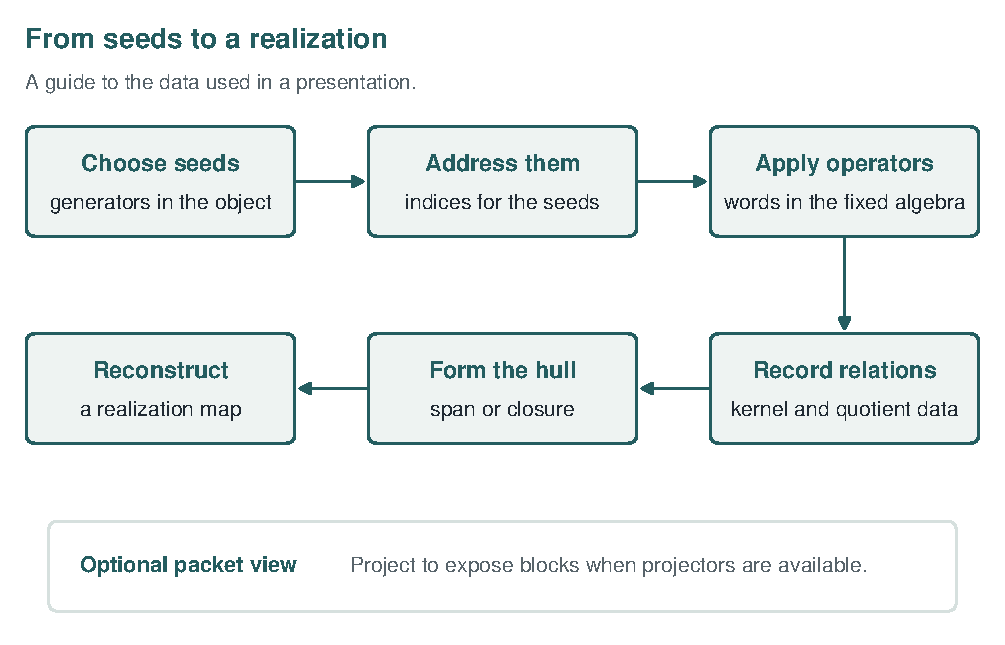
\includegraphics[width=0.96\textwidth]{01_seed_operator_grammar.pdf}
\caption{Schematic organization of the seed, operator, relation, and reconstruction data. This is a guide to the presentation, not an additional formal theorem.}
\label{fig:grammar}
\end{figure}

\section{Free presentations by seeds and relations}
\begin{readerroadmap}
A seed family gives a canonical map from a finite free module.  The generated hull is exactly its image, and the relations among addressed seeds form the kernel.  This converts orbit generation into a presentation problem.
\end{readerroadmap}
\subsection{Finite free covers}
\begin{definition}[Seed evaluation map]
\label{def:seed-evaluation}
Let $A$ be a unital ring, let $M$ be a left module over $A$, and let $S=(s_1,\ldots,s_r)\in M^r$.  Define the linear map over $A$
\[
\varepsilon_S:A^{\oplus r}\longrightarrow M,
\qquad
(a_1,\ldots,a_r)\longmapsto\sum_{j=1}^{r}a_js_j.
\]
\end{definition}
\RecordID{PSC-I-D-SEED-EVALUATION}

\begin{theorem}[Finite free presentation]
\label{thm:free-presentation}
For the map in \cref{def:seed-evaluation},
\[
\im\varepsilon_S=\Hull_A(S),
\qquad
N_S:=\Ker\varepsilon_S\leq A^{\oplus r},
\]
and the induced map is an isomorphism of left modules over $A$
\[
\boxed{A^{\oplus r}/N_S\cong\Hull_A(S).}
\]
Consequently, $S$ generates $M$ if and only if $\varepsilon_S$ is surjective.
\end{theorem}
\RecordID{PSC-I-T-FREE-PRESENTATION}
\Depends{PSC-I-D-SEED-EVALUATION and the first isomorphism theorem.}
\Exports{All later free seed presentations.}

\begin{proof}
The image consists exactly of finite sums $\sum_ja_js_j$, which is $\Hull_A(S)$.  Because $\varepsilon_S$ is linear over $A$, its kernel is a left submodule.  The first isomorphism theorem gives
\[
A^{\oplus r}/N_S\cong\im\varepsilon_S=\Hull_A(S).
\]
The final equivalence is the equality $\im\varepsilon_S=M$.
\end{proof}

\begin{interpretation}
The theorem converts the geometric language of addressed seed orbits into the algebraic language of generators and relations.  A word in the operators is represented by an element of the free module.  Two addressed expressions represent the same vector exactly when their difference lies in the kernel.  The generated hull is therefore not merely spanned by the free module.  It is its canonical quotient.
\end{interpretation}

\begin{microexample}[title={A cyclic nilpotent chain}]
Let \(A=\bbk[t]\) and \(M=\bbk[t]/(t^3)\).  The residue class \(s=[1]\) is one seed and
\[
\varepsilon_s:A\to M,
\qquad
f(t)\mapsto f(t)[1]
\]
has kernel \((t^3)\).  Hence \(M\cong A/(t^3)\), and the addressed vectors \(s,ts,t^2s\) are the visible orbit chain.
\end{microexample}


\begin{corollary}[Characterization by minimal free covers]
\label{cor:minimal-free-cover}
For every finitely generated left module $M$ over $A$,
\[
\boxed{
\srank_A(M)=\min\{r\geq0:\text{there exists a surjection }A^{\oplus r}\twoheadrightarrow M\}.
}
\]
\end{corollary}
\RecordID{PSC-I-C-MINIMAL-FREE-COVER}
\Depends{PSC-I-T-FREE-PRESENTATION.}

\begin{proof}
A seed family of size $r$ gives a surjection by \cref{thm:free-presentation}.  Conversely, the images of the standard basis vectors under any surjection $A^{\oplus r}\twoheadrightarrow M$ form a generating family of size at most $r$.
\end{proof}

\begin{corollary}[Presentation with one seed]
\label{cor:one-seed-presentation}
For $s\in M$, the annihilator
\[
\operatorname{Ann}_A(s):=\{a\in A:as=0\}
\]
is a left ideal and
\[
\boxed{A/\operatorname{Ann}_A(s)\cong\Hull_A(s).}
\]
\end{corollary}
\RecordID{PSC-I-C-ONE-SEED-PRESENTATION}
\Depends{PSC-I-T-FREE-PRESENTATION.}

\begin{proof}
The evaluation map for one seed is $a\mapsto as$.  Its kernel is $\operatorname{Ann}_A(s)$, which is therefore a left ideal, and \cref{thm:free-presentation} gives the quotient isomorphism.
\end{proof}

\subsection{One seed and the distinction between module and algebra relations}
\begin{proposition}[Criterion for the annihilator to be an ideal on both sides]
\label{prop:two-sided-annihilator}
For $s\in M$, the left ideal $L=\operatorname{Ann}_A(s)$ is an ideal on both sides if and only if
\[
L\,\Hull_A(s)=0.
\]
If $s$ is cyclic, these conditions are equivalent to
\[
\operatorname{Ann}_A(s)=\operatorname{Ann}_A(M).
\]
\end{proposition}
\RecordID{PSC-I-P-ANNIHILATOR-TWO-SIDED}
\Depends{PSC-I-C-ONE-SEED-PRESENTATION.}

\begin{proof}
The left ideal $L$ is an ideal on both sides exactly when $ab\in L$ for every $a\in L$ and $b\in A$.  This is equivalent to
\[
0=(ab)s=a(bs)
\qquad(a\in L,\ b\in A).
\]
By additivity, the last identity is equivalent to $L\Hull_A(s)=0$.

If $s$ is cyclic, then $\Hull_A(s)=M$.  Hence the preceding condition is $L\subseteq\operatorname{Ann}_A(M)$.  The reverse inclusion always holds because an operator annihilating all of $M$ annihilates $s$.  Thus equality follows.  Conversely, $\operatorname{Ann}_A(M)$ is an ideal on both sides, so equality implies that $L$ is an ideal on both sides.
\end{proof}

\begin{microexample}[title={Why a seed annihilator need not be an ideal on both sides}]
Let \(A=M_2(\bbk)\) act on \(M=\bbk^2\), and let \(s=e_1\).  Then \(\operatorname{Ann}_A(s)\) consists of matrices whose first column is zero.  It is a left ideal because left multiplication preserves a zero first column.  It is not generally a right ideal.  Thus the natural quotient for one seed is a quotient of the left regular module, not automatically a quotient algebra.
\end{microexample}


\subsection{Topological completion of a presentation}
\begin{theorem}[Completion of a dense free presentation]
\label{thm:completed-presentation}
Let $X$ be a complete Hausdorff locally convex space, let $\A\subseteq\End(X)$ act continuously, and let $S=(s_1,\ldots,s_r)$.  Put
\[
E:=\A^{\oplus r}/N_S
\]
algebraically and let $j:E\to X$ be the injective map induced by $\varepsilon_S$.  Give $E$ the locally convex topology transported from $j(E)$, equivalently the topology generated by
\[
\widetilde p(e):=p(j(e))
\]
for the continuous seminorms $p$ on $X$.  Every $a\in\A$ acts continuously on $E$ in the transported topology and therefore extends to $\widehat E$.  If $\Hull_{\A}(S)$ is dense in $X$, then $j$ extends uniquely to a topological isomorphism of modules over $\A$
\[
\boxed{\widehat E\cong X.}
\]
\end{theorem}
\RecordID{PSC-I-T-COMPLETED-PRESENTATION}
\Depends{PSC-I-T-FREE-PRESENTATION and uniqueness of Hausdorff completion.}

\begin{proof}
By \cref{thm:free-presentation}, $j$ is an algebraic isomorphism of modules over $\A$ from $E$ onto $\Hull_{\A}(S)$.  The transported seminorms make it a topological isomorphism onto that subspace.  For $a\in\A$ and a continuous seminorm $p$ on $X$, continuity of $a:X\to X$ supplies continuous seminorms controlling $p(aj(e))$, so the induced action on $E$ is continuous and extends uniquely to $\widehat E$.  The subspace is dense by hypothesis.  A Cauchy net in $E$ is mapped to a Cauchy net in $X$, which converges because $X$ is complete.  This defines a continuous extension $\widehat j:\widehat E\to X$.  For any $x\in X$, choose a net $(e_\lambda)$ in $E$ with $j(e_\lambda)\to x$.  The transported topology makes $(e_\lambda)$ Cauchy, so it converges to some $\xi\in\widehat E$, and continuity gives $\widehat j(\xi)=x$.  Thus $\widehat j$ is surjective.  If $\widehat j(\xi)=0$, represent $\xi$ by a Cauchy net $(e_\lambda)$.  Then $j(e_\lambda)\to0$, so every defining seminorm $\widetilde p(e_\lambda)$ tends to zero.  Thus $e_\lambda\to0$ in the completion and $\xi=0$.  Hence $\widehat j$ is bijective.  Its inverse is continuous by the universal property of completion, or directly because the topology on $E$ was transported from $X$.
\end{proof}

The topology in this completion theorem comes from the realized image.  It is not an independently chosen topology on the free algebra.  This choice ensures that the completion recovers the given space, while leaving separate the question of whether another natural topology on the grammar produces the same completion.

\begin{sectionrecap}
A seed family always gives a free presentation of its hull.  The kernel stores all linear relations among addressed seed words.  One seed gives a cyclic module, but only special annihilators permit an algebra quotient.  Dense generation is handled by completing the presented image rather than by silently replacing algebraic span with closure.
\end{sectionrecap}

\section{Seed rank and functorial calculus}



\begin{readerroadmap}
For a finitely generated module, seed rank is the smallest number of seeds needed to generate it.  We first examine how this number behaves when the acting algebra changes or the module is replaced by a quotient.  We then give bounds for exact sequences, direct sums, and tensor products.  Quotients with simple actions provide useful witnesses for lower bounds.
\end{readerroadmap}
\subsection{Definition, cyclicity, and monotonicity}

\begin{definition}[Seed rank]
\label{def:seed-rank}
For a unital left module $M$ over $A$, define
\[
\srank_A(M):=\min\{|S|:AS=M\}.
\]
For a topological module $(X,\tau)$, define
\[
\srank_{\A,\tau}(X):=\min\{|S|:\cl{\A S}^{\,\tau}=X\}.
\]
Set $\srank_A(0)=0$.  When the value is finite, it is the minimal number of module generators.
\end{definition}
\RecordID{PSC-I-D-SEED-RANK}

\begin{proposition}[Cyclic characterization]
\label{prop:cyclic-characterization}
For $M\neq0$,
\[
\srank_A(M)=1
\quad\Longleftrightarrow\quad
M\text{ contains a cyclic vector}.
\]
\end{proposition}
\RecordID{PSC-I-P-CYCLIC-CHARACTERIZATION}
\Depends{PSC-I-D-SEED-RANK.}

\begin{proof}
Both conditions say that there is $m\in M$ with $Am=M$.
\end{proof}

\begin{proposition}[Monotonicity under enlargement of the acting algebra]
\label{prop:acting-algebra-monotonicity}
Let $B\subseteq A\subseteq\End_{\bbk}(X)$ be unital operator algebras with the same identity.  Then
\[
\boxed{\srank_A(X)\leq\srank_B(X).}
\]
The same statement holds for topological seed rank when both algebras act continuously.
\end{proposition}
\RecordID{PSC-I-P-ACTING-ALGEBRA-MONOTONICITY}
\Depends{PSC-I-D-SEED-RANK.}

\begin{proof}
For every $S\subseteq X$, one has $BS\subseteq AS$.  Hence every generating family over $B$ is also a generating family over $A$.  Taking closures gives the topological statement.
\end{proof}

\begin{interpretation}
Enlarging the acting algebra can only create more orbit directions, so it can only lower the number of seeds required.  This is why every statement about seed rank must name the acting algebra.  The same vector space may be cyclic for a large algebra and require many seeds for a smaller one.
\end{interpretation}


\subsection{Quotients, isomorphisms, and exact sequences}
\begin{theorem}[Quotient monotonicity]
\label{thm:quotient-monotonicity}
Let $\varphi:A\to B$ be a unital ring homomorphism and let
\[
\Phi:M\twoheadrightarrow N
\]
be a surjective additive map satisfying
\[
\Phi(am)=\varphi(a)\Phi(m)
\qquad(a\in A,\ m\in M).
\]
Then
\[
\boxed{\srank_B(N)\leq\srank_A(M).}
\]
If $M$ and $N$ are topological modules, $\Phi$ is continuous and surjective, and the actions are continuous, then
\[
\srank_{B,\tau_N}(N)\leq\srank_{A,\tau_M}(M).
\]
\end{theorem}
\RecordID{PSC-I-T-QUOTIENT-MONOTONICITY}
\Depends{PSC-I-D-GENERATED-HULL and PSC-I-D-SEED-RANK.}
\Exports{All quotient lower bounds and realization inequalities.}

\begin{proof}
Let $S$ generate $M$.  For every $n\in N$, choose $m\in M$ with $\Phi(m)=n$ and write $m=\sum_ia_is_i$.  Then
\[
n=\sum_i\varphi(a_i)\Phi(s_i),
\]
so $\Phi(S)$ generates $N$.

For the topological statement, let $S$ generate $M$ densely.  Given $n=\Phi(m)$, choose a net $m_\lambda\in AS$ converging to $m$.  Continuity gives
\[
\Phi(m_\lambda)\longrightarrow n,
\]
and every $\Phi(m_\lambda)$ lies in $B\Phi(S)$.  Thus $B\Phi(S)$ is dense in $N$.
\end{proof}

\begin{microexample}[title={A quotient can strictly lower seed rank}]
Let \(A=\bbk\) act by scalars on \(M=\bbk^3\).  Then \(\srank_A(M)=3\).  Quotienting by a subspace of dimension one gives a scalar module of dimension two, whose seed rank is \(2\).  Quotient monotonicity is therefore often strict.
\end{microexample}


\begin{corollary}[Isomorphism invariance]
\label{cor:isomorphism-invariance}
An intertwining module isomorphism preserves algebraic seed rank.  A topological intertwining isomorphism preserves topological seed rank.
\end{corollary}
\RecordID{PSC-I-C-ISOMORPHISM-INVARIANCE}
\Depends{PSC-I-T-QUOTIENT-MONOTONICITY.}

\begin{proof}
Apply \cref{thm:quotient-monotonicity} to the isomorphism and its inverse.
\end{proof}

\begin{theorem}[Short exact sequence bounds]
\label{thm:exact-sequence-bounds}
Let
\[
0\longrightarrow L\xrightarrow{\iota}M\xrightarrow{\pi}N\longrightarrow0
\]
be a short exact sequence of left modules over $A$.  Then
\[
\boxed{
\srank_A(N)\leq\srank_A(M)
\leq\srank_A(L)+\srank_A(N).
}
\]
\end{theorem}
\RecordID{PSC-I-T-EXACT-SEQUENCE-BOUNDS}
\Depends{PSC-I-T-QUOTIENT-MONOTONICITY.}

\begin{proof}
The lower inequality is quotient monotonicity. For the upper inequality, choose generating families $(\ell_i)_{i\in I}$ of $L$ and $(n_j)_{j\in J}$ of $N$ with the least possible cardinalities. Choose a lift $m_j\in M$ of each $n_j$. For any $m\in M$, a finite subset $F\subseteq J$ and coefficients $a_j\in A$ give
\[
\pi(m)=\sum_{j\in F}a_jn_j.
\]
The vector $m-\sum_{j\in F}a_jm_j$ belongs to $\iota(L)$, so it is a finite linear combination of the $\iota(\ell_i)$. The union of the lifted family and the image of the generating family of $L$ therefore generates $M$. Its cardinality is at most $|I|+|J|$, giving the upper bound. This argument uses finite sums for each vector even when either generating family is infinite.
\end{proof}

\begin{hypothesisguide}
For a short exact sequence, a generating family for \(M\) always maps to a generating family for the quotient.  It need not generate the submodule \(L\).  For the upper bound, choose generators of \(L\) separately and combine them with lifts of quotient generators.
\end{hypothesisguide}


\subsection{Direct sums under shared and independent actions}
\begin{proposition}[Direct sum bounds for a shared action]
\label{prop:shared-direct-sum}
If one algebra $A$ acts diagonally on $M\oplus N$, then
\[
\boxed{
\max\{\srank_A(M),\srank_A(N)\}
\leq\srank_A(M\oplus N)
\leq\srank_A(M)+\srank_A(N).
}
\]
\end{proposition}
\RecordID{PSC-I-P-SHARED-DIRECT-SUM}
\Depends{PSC-I-T-QUOTIENT-MONOTONICITY.}

\begin{proof}
The coordinate projections are intertwining quotients and give the lower bound.  For the upper bound, embed minimal generating families of $M$ as $(m_i,0)$ and of $N$ as $(0,n_j)$. Their union generates by finite sums and has cardinality at most the sum of the two seed ranks.
\end{proof}

\begin{theorem}[Direct sum formula for independent actions]
\label{thm:independent-direct-sum}
Let $M$ be a left module over $A$ and $N$ a left module over $B$.  Under the action of the product algebra
\[
(a,b)(m,n)=(am,bn),
\]
one has
\[
\boxed{
\srank_{A\times B}(M\oplus N)
=
\max\{\srank_A(M),\srank_B(N)\}.
}
\]
\end{theorem}
\RecordID{PSC-I-T-INDEPENDENT-DIRECT-SUM}
\Depends{PSC-I-T-QUOTIENT-MONOTONICITY.}

\begin{proof}
The coordinate projections give the lower bound. Let $r$ be the maximum on the right, regarded as a cardinal, and choose an index set $I$ of cardinality $r$. Choose minimal generating families for $M$ and $N$, index them by subsets of $I$, and fill any unused positions with zeros. Write the resulting families as $(m_i)_{i\in I}$ and $(n_i)_{i\in I}$. For any $m\in M$ and $n\in N$, their finite expressions involve a common finite subset $F\subseteq I$ after zero coefficients have been added. Thus
\[
m=\sum_{i\in F}a_im_i,
\qquad
n=\sum_{i\in F}b_in_i,
\]
and
\[
(m,n)=\sum_{i\in F}(a_i,b_i)(m_i,n_i).
\]
The family of paired vectors generates and has cardinality at most $r$. The empty family handles the case in which both modules are zero.
\end{proof}

\subsection{Tensor generation and witnesses for lower bounds}
\begin{proposition}[Tensor product bound]
\label{prop:tensor-bound}
Let $A$ and $B$ be unital algebras over $\bbk$, let $M$ be a left module over $A$, and let $N$ be a left module over $B$.  Under the natural $A\otimes_{\bbk}B$ action,
\[
\boxed{
\srank_{A\otimes B}(M\otimes_{\bbk}N)
\leq
\srank_A(M)\srank_B(N).
}
\]
\end{proposition}
\RecordID{PSC-I-P-TENSOR-BOUND}
\Depends{PSC-I-D-SEED-RANK.}

\begin{proof}
Choose minimal generating families $(m_i)_{i\in I}$ for $M$ and $(n_j)_{j\in J}$ for $N$. Each vector in either module is a finite linear combination of its generators. Bilinearity therefore expresses every simple tensor as a finite sum of terms
\[
(am_i)\otimes(bn_j)=(a\otimes b)(m_i\otimes n_j).
\]
Simple tensors span the algebraic tensor product, so the family $(m_i\otimes n_j)_{(i,j)\in I\times J}$ generates it. This family has cardinality at most $|I||J|$, which is the claimed bound. The proof also covers an empty generating family, when the corresponding module and tensor product are zero.
\end{proof}

\begin{interpretation}
The tensor product bound is constructive.  Tensor the chosen seed families and act independently in the two factors.  Equality can fail because a single tensor seed may contain several useful components, or because the tensor product algebra acquires additional relations.  Later quantum applications should therefore cite the bound, not assume multiplicativity.
\end{interpretation}


\begin{boundary}[Tensor rank is not generally multiplicative]
\label{bnd:tensor-nonequality}
The inequality in \cref{prop:tensor-bound} can be strict.  Equality requires additional hypotheses on the acting algebras and their module multiplicities and is not exported as a universal law.
\end{boundary}
\RecordID{PSC-I-B-TENSOR-NONEQUALITY}



\begin{proposition}[Monotonicity under extension of scalars]
\label{prop:scalar-extension}
Let \(K/\bbk\) be a field extension, let \(A\) be a unital algebra over \(\bbk\), and let \(M\) be a finitely generated left module over \(A\).  Set
\[
A_K:=K\otimes_{\bbk}A,
\qquad
M_K:=K\otimes_{\bbk}M.
\]
Then
\[
\boxed{
\srank_{A_K}(M_K)\leq\srank_A(M).
}
\]
Every generating family \(S\subseteq M\) extends to the generating family \(1\otimes S\subseteq M_K\).
\end{proposition}
\RecordID{PSC-I-P-SCALAR-EXTENSION-MONOTONICITY}
\Depends{PSC-I-D-SEED-RANK.}
\Exports{Extension of the coefficient field in realizations from arithmetic, quantum theory, and representation theory.}

\begin{proof}
Let \(S=\{s_1,\ldots,s_r\}\) generate \(M\).  Every pure tensor \(\lambda\otimes m\in M_K\) has an expression
\[
m=\sum_{i=1}^r a_is_i,
\]
so
\[
\lambda\otimes m
=
\sum_{i=1}^r(\lambda\otimes a_i)(1\otimes s_i).
\]
Pure tensors span \(M_K\), hence \(1\otimes S\) generates \(M_K\) over \(A_K\).  Taking the minimum over \(S\) proves the inequality.
\end{proof}

\begin{hypothesisguide}
The proposition gives an inequality in one direction.  A smaller generating family found after extending scalars need not descend to the original field.  Descent requires additional structure.  The chapter therefore exports monotonicity, not an unconditional equality.
\end{hypothesisguide}


\subsection{Quotient witnesses for lower bounds}
\begin{definition}[Witness for seed rank]
\label{def:seed-rank-witness}
A surjective intertwiner $\Phi:M\twoheadrightarrow N$ is a witness for seed rank of order $r$ when $\srank(N)=r$.  It certifies $\srank(M)\geq r$.
\end{definition}
\RecordID{PSC-I-D-SEED-RANK-WITNESS}

\begin{proposition}[Scalar quotient witness]
\label{prop:scalar-quotient}
Let $M$ be a module over $A$ with coefficient field $\bbk$.  Suppose $M$ has a quotient $N$ of dimension $r$ on which $A$ acts through a character
\[
\chi:A\longrightarrow\bbk.
\]
Then
\[
\boxed{\srank_A(M)\geq r.}
\]
\end{proposition}
\RecordID{PSC-I-P-SCALAR-QUOTIENT-WITNESS}
\Depends{PSC-I-T-QUOTIENT-MONOTONICITY.}

\begin{proof}
For every $n\in N$, the cyclic submodule $An$ is contained in the scalar span $\bbk n$.  Therefore $q$ seed images span a subspace of dimension at most $q$.  Generating the quotient of dimension $r$ requires at least $r$ seeds.  Quotient monotonicity transfers the lower bound to $M$.
\end{proof}

\begin{sectionrecap}
Seed rank is functorial under quotients and isomorphisms, subadditive across extensions, given by the maximum for independent product actions, and bounded above under tensor products.  Lower bounds come from quotients on which the action simplifies.  Scalar extension cannot increase seed rank, but descent of a reduced seed family is a separate problem.
\end{sectionrecap}

\section{Generator number modulo the Jacobson radical}



\begin{readerroadmap}
For a finitely generated module, Nakayama's lemma allows us to count generators after passing to the quotient by the Jacobson radical.  When the algebra has finite dimension, this quotient is semisimple and its multiplicities give an explicit answer.  We begin with the radical reduction and then calculate those multiplicities.
\end{readerroadmap}
\subsection{Reduction to the module top}

\begin{classicalinput}[Nakayama lemma]
\label{ci:nakayama}
Let $A$ be a unital ring, let $J\subseteq\Jac(A)$, and let $M$ be a finitely generated left module over $A$.  If $M=N+JM$ for a submodule $N\leq M$, then $M=N$.
\end{classicalinput}
\RecordID{PSC-I-CI-NAKAYAMA}

\begin{theorem}[Generator number is detected modulo the Jacobson radical]
\label{thm:module-top}
Let $A$ be a unital ring, let $J=\Jac(A)$, and let $M$ be a finitely generated left module over $A$.  A family $S\subseteq M$ generates $M$ if and only if its image generates $M/JM$ as a module over $A/J$.  When $A/J$ is semisimple Artinian, this quotient is the usual semisimple top.  No semisimplicity of $A/J$ is required for the general equality.  Consequently,
\[
\boxed{
\srank_A(M)=\srank_{A/J}(M/JM).
}
\]
\end{theorem}
\RecordID{PSC-I-T-MODULE-TOP}
\Depends{PSC-I-CI-NAKAYAMA and PSC-I-T-QUOTIENT-MONOTONICITY.}
\Exports{Generator formulas in finite dimension, quantum multiplicity calculations, and residual deformation modules.}

\begin{proof}
If $S$ generates $M$, its image generates every quotient.  Conversely, suppose the image of $S$ generates $M/JM$ and put $N=AS$.  Then
\[
M=N+JM.
\]
Nakayama's lemma gives $M=N$.  Thus the same finite families generate before and after passage to the top, and the minimal cardinalities agree.
\end{proof}

\begin{interpretation}
The theorem says that nilpotent or radical directions can lengthen orbit chains but cannot reduce the number of independent directions in the module top that must be seeded.  Once the images of the seeds generate \(M/JM\), Nakayama's lemma forces the entire module to be generated.
\end{interpretation}

\begin{microexample}[title={A local nilpotent algebra}]
Let \(A=\bbk[\varepsilon]/(\varepsilon^3)\) and \(M=A^{\oplus2}\).  The radical is \(J=(\varepsilon)\), and
\[
M/JM\cong\bbk^2.
\]
Therefore two seeds are necessary and sufficient.  The extra nilpotent layers \(\varepsilon M\) and \(\varepsilon^2M\) are generated automatically once the two top directions are seeded.
\end{microexample}


\begin{corollary}[Local algebra formula]
\label{cor:local-algebra-formula}
Let $A$ be a local ring with Jacobson radical $J$ and residue division ring $D=A/J$.  For every finitely generated left module $M$ over $A$,
\[
\boxed{
\srank_A(M)=\dim_D(M/JM),
}
\]
where the dimension is that of a left vector space over $D$.
\end{corollary}
\RecordID{PSC-I-C-LOCAL-ALGEBRA-FORMULA}
\Depends{PSC-I-T-MODULE-TOP.}

\begin{proof}
The module $M/JM$ over $A/J$ is a left vector space over $D$.  Its minimal number of generators is its dimension over $D$.
\end{proof}

\subsection{Semisimple multiplicity calculus}
\begin{classicalinput}[Wedderburn and Artin decomposition]
\label{ci:wedderburn}
Every semisimple Artinian ring is isomorphic to a finite product
\[
A\cong\prod_{i=1}^{q}M_{d_i}(D_i)
\]
of full matrix rings over division rings.
\end{classicalinput}
\RecordID{PSC-I-CI-WEDDERBURN-ARTIN}

\begin{lemma}[Multiplicities in the regular module]
\label{lem:regular-multiplicities}
Let
\[
A=\prod_{i=1}^{q}M_{d_i}(D_i)
\]
and let $S_i=D_i^{d_i}$ denote the natural simple left module for the $i$th factor, extended by zero across the other factors.  Then, as a left module over $A$,
\[
\boxed{A\cong\bigoplus_{i=1}^{q}S_i^{\oplus d_i}.}
\]
\end{lemma}
\RecordID{PSC-I-L-REGULAR-MODULE-MULTIPLICITIES}
\Depends{PSC-I-CI-WEDDERBURN-ARTIN.}

\begin{proof}
For one factor $M_d(D)$, let $e_{jj}$ be the diagonal matrix units.  The left regular module decomposes as
\[
M_d(D)=\bigoplus_{j=1}^{d}M_d(D)e_{jj}.
\]
Each minimal left ideal $M_d(D)e_{jj}$ is isomorphic to the natural column module $D^d$.  Taking the direct product of factors gives the stated decomposition.
\end{proof}

\begin{theorem}[Semisimple seed rank formula over arbitrary division rings]
\label{thm:semisimple-seed-rank}
Let
\[
A\cong\prod_{i=1}^{q}M_{d_i}(D_i)
\]
be semisimple Artinian and let
\[
M\cong\bigoplus_{i=1}^{q}S_i^{\oplus m_i}
\]
be a finitely generated left module over $A$.  Then
\[
\boxed{
\srank_A(M)
=
\max_{1\leq i\leq q}
\left\lceil\frac{m_i}{d_i}\right\rceil.
}
\]
If $A$ is any algebra of finite dimension over a field, the same formula applied to the decomposition of $M/\Jac(A)M$ over $A/\Jac(A)$ computes $\srank_A(M)$.
\end{theorem}
\RecordID{PSC-I-T-SEMISIMPLE-SEED-RANK}
\Depends{PSC-I-T-MODULE-TOP, PSC-I-CI-WEDDERBURN-ARTIN, PSC-I-L-REGULAR-MODULE-MULTIPLICITIES, and PSC-I-C-MINIMAL-FREE-COVER.}
\Exports{Every calculation of seed rank for semisimple algebras of finite dimension in the series.}

\begin{proof}
By \cref{cor:minimal-free-cover}, $M$ is generated by $r$ elements exactly when it is a quotient of $A^{\oplus r}$.  By \cref{lem:regular-multiplicities},
\[
A^{\oplus r}\cong\bigoplus_iS_i^{\oplus rd_i}.
\]
Every short exact sequence of modules over a semisimple ring splits.  Therefore a quotient isomorphic to $M$ exists if and only if
\[
m_i\leq rd_i
\qquad\text{for every }i.
\]
The smallest such $r$ is the displayed maximum.  For a nonsemisimple algebra of finite dimension, \cref{thm:module-top} reduces the calculation to the semisimple module $M/\Jac(A)M$ over $A/\Jac(A)$.
\end{proof}

\begin{interpretation}
For the factor \(M_{d_i}(D_i)\), one free generator contributes \(d_i\) copies of the corresponding simple module.  If the top of \(M\) contains \(m_i\) copies, at least \(\lceil m_i/d_i\rceil\) free generators are required.  The worst simple type controls the global answer.

This count concerns copies of a simple module, rather than the number of coordinates in a chosen basis.  A single seed can reach several copies through the matrix action.  The regular module records precisely how many copies one free generator can supply.
\end{interpretation}

\begin{microexample}[title={Multiplicity consumes seed capacity}]
For \(A=M_2(\bbk)\) acting on \((\bbk^2)^{\oplus3}\), the regular module contributes two copies of the natural simple module per generator.  One generator cannot cover all three multiplicity directions.  Two can, giving seed rank \(2\).
\end{microexample}


\Needspace{16\baselineskip}
\begin{corollary}[Algebraically closed multiplicity formula]
\label{cor:algebraically-closed-formula}
Let $\bbk$ be algebraically closed, let $A$ be a unital algebra of finite dimension over $\bbk$, put $J=\Jac(A)$, and let $M$ be a finitely generated left module over $A$.  Assume compatible decompositions indexed by an integer $q\geq0$:
\[
A/J\cong\prod_{i=1}^{q}M_{d_i}(\bbk),
\qquad
M/JM\cong\bigoplus_{i=1}^{q}(\bbk^{d_i})^{\oplus m_i},
\]
where the $d_i$ are positive integers and the $m_i$ are nonnegative integers.  The first isomorphism is an isomorphism of algebras over $\bbk$.  The second is an isomorphism of left modules over $A/J$, using the natural column module for each matrix factor and zero action from the other factors.  Then
\[
\srank_A(M)=\max_{1\leq i\leq q}\left\lceil\frac{m_i}{d_i}\right\rceil,
\]
with $\max\varnothing=0$ when $q=0$.
\end{corollary}
\RecordID{PSC-I-C-ALGEBRAICALLY-CLOSED-FORMULA}
\Depends{PSC-I-T-MODULE-TOP and PSC-I-T-SEMISIMPLE-SEED-RANK.}

\begin{proof}
By \cref{thm:module-top}, $\srank_A(M)=\srank_{A/J}(M/JM)$.  Apply \cref{thm:semisimple-seed-rank} to the displayed decompositions of $A/J$ and $M/JM$, with every $D_i=\bbk$.  This gives the stated maximum.  If $q=0$, the unital $A/J$-module $M/JM$ is zero, and \cref{thm:module-top} gives seed rank zero.
\end{proof}

\begin{corollary}[Full matrix algebra]
\label{cor:full-matrix}
For the natural module $S=D^d$ over $M_d(D)$,
\[
\srank_{M_d(D)}(S)=1.
\]
More strongly, every nonzero vector of $S$ is cyclic.
\end{corollary}
\RecordID{PSC-I-C-FULL-MATRIX}
\Depends{PSC-I-T-SEMISIMPLE-SEED-RANK.}

\begin{proof}
The formula gives $\lceil1/d\rceil=1$.  Directly, let $v\neq0$ and choose a coordinate $v_j\neq0$.  For any target $w=(w_i)$, the matrix whose $j$th column has entries $w_iv_j^{-1}$ and whose other columns vanish sends $v$ to $w$.
\end{proof}

\begin{corollary}[Multiplicity obstruction]
\label{cor:multiplicity-obstruction}
For the diagonal action of $M_d(D)$ on $S^{\oplus m}$,
\[
\boxed{
\srank_{M_d(D)}(S^{\oplus m})
=
\left\lceil\frac{m}{d}\right\rceil.
}
\]
\end{corollary}
\RecordID{PSC-I-C-MULTIPLICITY-OBSTRUCTION}
\Depends{PSC-I-T-SEMISIMPLE-SEED-RANK.}

\begin{proof}
Apply \cref{thm:semisimple-seed-rank} to the single simple type with multiplicity $m$.
\end{proof}

\begin{sectionrecap}
For finitely generated modules, the minimal number of seeds is detected on the quotient by the Jacobson radical.  In the semisimple top, each generator has a fixed multiplicity capacity \(d_i\) in simple type \(i\), and the largest capacity ratio determines the exact seed rank.
\end{sectionrecap}

\begin{figure}[htbp]
\centering
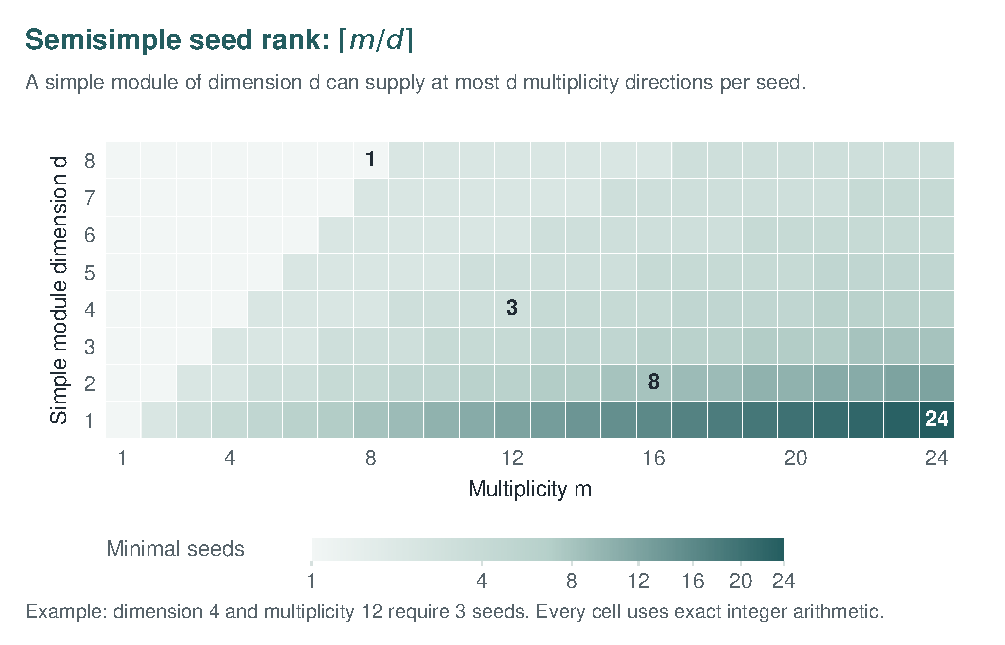
\includegraphics[width=0.96\textwidth]{04_semisimple_seed_rank.pdf}
\caption{The semisimple multiplicity formula for one simple block. A seed can expose at most $d$ independent multiplicity directions, so $m$ copies require $\lceil m/d\rceil$ seeds.}
\label{fig:semisimple}
\end{figure}

\section{Modules for a single operator over arbitrary fields}



\begin{readerroadmap}
One operator is equivalent to a module over \(\bbk[t]\).  Primary decomposition isolates the irreducible polynomial sectors, and the quotient by \(p(T)\) counts how many cyclic chains begin in each sector.
\end{readerroadmap}
\subsection{Primary components and generator counts}

\begin{classicalinput}[Primary decomposition for polynomial modules]
\label{ci:primary-decomposition}
Every module $X$ over $\bbk[t]$ with finite dimension over the coefficient field decomposes as
\[
X=\bigoplus_{p\in\Irr(\bbk[t])}X_p,
\]
where $\Irr(\bbk[t])$ denotes the monic irreducible polynomials, only finitely many components are nonzero, and every nonzero $X_p$ is a finite direct sum of modules $\bbk[t]/(p^e)$.
\end{classicalinput}
\RecordID{PSC-I-CI-PID-PRIMARY-DECOMPOSITION}

\begin{theorem}[Seed rank for a single operator]
\label{thm:single-operator}
Let $X$ have finite dimension over $\bbk$ and let $T\in\End_{\bbk}(X)$.  Regard $X$ as a module over $\bbk[t]$ by $t\cdot x=Tx$.  For every monic irreducible $p$, let $X_p$ be the primary component for $p$ and set
\[
\mu_p(T):=
\dim_{\bbk[t]/(p)}\bigl(X_p/p(T)X_p\bigr).
\]
Then
\[
\boxed{
\srank_{\bbk[T]}(X)=\max_p\mu_p(T).
}
\]
Moreover, $\mu_p(T)$ is the number of cyclic primary summands for $p$ in the decomposition into elementary divisors of $X_p$.
\end{theorem}
\RecordID{PSC-I-T-SINGLE-OPERATOR}
\Depends{\nolinkurl{PSC-I-CI-PID-PRIMARY-DECOMPOSITION},
\nolinkurl{PSC-I-C-LOCAL-ALGEBRA-FORMULA}, and
\nolinkurl{PSC-I-T-INDEPENDENT-DIRECT-SUM}.}
\Exports{Companion, recurrence, and systems of subsequences in residue classes.}

\begin{proof}
Let the minimal polynomial be
\[
m_T(t)=\prod_{p}p(t)^{e_p}.
\]
The acting algebra is
\[
\bbk[T]\cong\bbk[t]/(m_T)
\cong\prod_pR_p,
\qquad
R_p:=\bbk[t]/(p^{e_p}),
\]
by the Chinese remainder theorem.  The factor $R_p$ acts on $X_p$ and annihilates every other primary component.  Hence the formula for a direct sum with independent actions gives
\[
\srank_{\bbk[T]}(X)=\max_p\srank_{R_p}(X_p).
\]
Each $R_p$ is local with maximal ideal generated by the class of $p$ and residue division field $K_p=\bbk[t]/(p)$.  By \cref{cor:local-algebra-formula},
\[
\srank_{R_p}(X_p)
=
\dim_{K_p}X_p/p(T)X_p
=
\mu_p(T).
\]
Finally, every summand $\bbk[t]/(p^e)$ contributes one copy of $K_p$ after quotienting by $p$, so the dimension equals the number of summands in the elementary divisor decomposition.
\end{proof}

\begin{interpretation}
For one operator, the quotient \(X_p/p(T)X_p\) counts the number of independent primary chains for the irreducible polynomial \(p\).  Over an algebraic closure these become Jordan chains.  The seed rank is the largest chain count among the primary sectors, not the largest chain length.
\end{interpretation}

\begin{microexample}[title={Block count versus block size}]
A nilpotent operator with Jordan block sizes \((5,1,1)\) has seed rank \(3\), even though its largest block has length \(5\).  Three seeds are needed because there are three independent chains.  Once their initial vectors are chosen, repeated application of \(T\) generates every position in those chains.
\end{microexample}


\subsection{Invariant factors, Jordan blocks, and cyclicity}
\begin{corollary}[Invariant factor count]
\label{cor:invariant-factor-count}
If $X\neq0$ and the rational canonical decomposition is written with nonconstant invariant factors
\[
X\cong\bigoplus_{j=1}^{r}\bbk[t]/(f_j),
\qquad
f_1\mid f_2\mid\cdots\mid f_r,
\]
then
\[
\boxed{\srank_{\bbk[T]}(X)=r.}
\]
\end{corollary}
\RecordID{PSC-I-C-INVARIANT-FACTOR-COUNT}
\Depends{PSC-I-T-SINGLE-OPERATOR.}

\begin{proof}
For each irreducible $p$, the number of invariant factors divisible by $p$ equals the number of elementary divisors for $p$.  Because $f_1\mid\cdots\mid f_r$ and $f_1\neq1$ after zero summands are removed, some irreducible divisor of $f_1$ divides all $r$ invariant factors.  Hence $\max_p\mu_p(T)=r$.
\end{proof}

\begin{corollary}[Formula for geometric multiplicity]
\label{cor:geometric-multiplicity}
If $\bbk$ is algebraically closed, then
\[
\boxed{
\srank_{\bbk[T]}(X)
=
\max_{\lambda\in\operatorname{Spec}(T)}
\dim_{\bbk}\Ker(T-\lambda I).
}
\]
\end{corollary}
\RecordID{PSC-I-C-ALGEBRAICALLY-CLOSED-SINGLE-OPERATOR}
\Depends{PSC-I-T-SINGLE-OPERATOR.}

\begin{proof}
The irreducibles are $p=t-\lambda$.  On the primary component for $\lambda$, the quotient by $(T-\lambda I)X_\lambda$ has dimension equal to the number of Jordan blocks, which is also $\dim\Ker(T-\lambda I)$.
\end{proof}

\begin{corollary}[Criterion for a cyclic matrix]
\label{cor:cyclic-matrix}
For $X\ne0$ of finite dimension, the following are equivalent:
\begin{enumerate}[label=(\roman*)]
\item $T$ has a cyclic vector.
\item $\srank_{\bbk[T]}(X)=1$.
\item Every nonzero primary component for $p$ is cyclic.
\item The rational canonical form has one invariant factor.
\item The minimal polynomial equals the characteristic polynomial.
\item After scalar extension to an algebraic closure, every eigenvalue has geometric multiplicity one.
\end{enumerate}
\end{corollary}
\RecordID{PSC-I-C-CYCLIC-MATRIX}
\Depends{PSC-I-T-SINGLE-OPERATOR, PSC-I-C-INVARIANT-FACTOR-COUNT, and PSC-I-P-CYCLIC-CHARACTERIZATION.}

\begin{proof}
The equivalence of (i) and (ii) is \cref{prop:cyclic-characterization}.  By \cref{thm:single-operator}, (ii) holds exactly when every $\mu_p(T)$ belonging to a nonzero primary component equals one, which is (iii).  Relatively prime primary cyclic modules combine into one cyclic module by the Chinese remainder theorem, so (iii) is equivalent to (iv).  In rational canonical form, one invariant factor means that the unique invariant factor is both the minimal and characteristic polynomial, proving (iv)$\Leftrightarrow$(v).  Scalar extension preserves the equality of minimal and characteristic polynomials.  Over an algebraic closure, that equality is equivalent to one Jordan block for each eigenvalue, which is (vi).
\end{proof}

\begin{sectionrecap}
A single operator is cyclic exactly when each primary sector has one cyclic chain.  Over an algebraic closure this is equivalent to one Jordan block per eigenvalue and to equality of the minimal and characteristic polynomials.
\end{sectionrecap}

\begin{figure}[htbp]
\centering
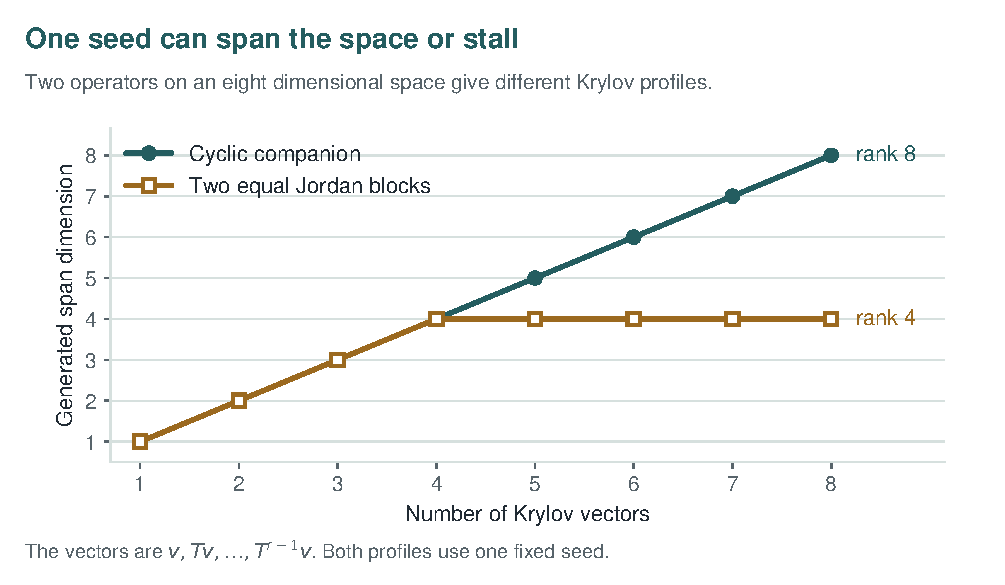
\includegraphics[width=0.96\textwidth]{03_cyclic_rank_profiles.pdf}
\caption{Krylov rank profiles for a cyclic companion operator and for two equal primary blocks. The second orbit stalls before reaching the ambient dimension because one seed cannot separate the repeated blocks.}
\label{fig:krylov}
\end{figure}


\section{Exact finite and countable packet coordinates}



\begin{readerroadmap}
Packets give exact coordinates through idempotent maps.  For finitely many packets, the reconstruction is algebraic.  For countably many packets, we must also specify how the series converges and bound the coordinate maps.  We begin with finite reconstruction, then consider packet support, tensor products, duality, and the universal mapping property before turning to convergence.
\end{readerroadmap}
\subsection{Finite exact packets}

\begin{definition}[Finite packet system]
\label{def:packet-system}
A finite packet system on a vector space $X$ over $\bbk$ is a family
\[
\Pcal=(P_\alpha)_{\alpha\in I}\subseteq\End_{\bbk}(X)
\]
satisfying
\[
P_\alpha^2=P_\alpha,
\qquad
P_\alpha P_\beta=0\quad(\alpha\neq\beta),
\qquad
\sum_{\alpha\in I}P_\alpha=I_X.
\]
Set $X_\alpha=P_\alpha X$.  Zero packet spaces may be removed without changing any identity.  No orthogonality is assumed unless stated.
\end{definition}
\RecordID{PSC-I-D-PACKET-SYSTEM}

\begin{definition}[Packet support and packet pure vectors]
\label{def:packet-support}
For a finite packet system \(\Pcal=(P_\alpha)_{\alpha\in I}\) and \(x\in X\), define
\[
\Supp_{\Pcal}(x)
:=
\{\alpha\in I:P_\alpha x\neq0\}.
\]
The vector \(x\) is \emph{packet pure} if \(|\Supp_{\Pcal}(x)|\leq1\).  A finite family is packet pure if each of its members is packet pure, although different members may lie in different packets.
\end{definition}
\RecordID{PSC-I-D-PACKET-SUPPORT}

\begin{interpretation}
Packet support records which packet coordinates are present.  A seed may lie in one packet, have coordinates in several packets, or be zero.  Later, when we count the seeds needed for generation, this distinction matters because a seed with several nonzero coordinates can meet several graph sources at once.
\end{interpretation}


\begin{lemma}[Finite packet aggregation]
\label{lem:packet-aggregation}
Let $\sigma:I\twoheadrightarrow J$ be a surjection and define
\[
Q_j:=\sum_{\sigma(\alpha)=j}P_\alpha.
\]
Then $(Q_j)_{j\in J}$ is a finite packet system and
\[
Q_jX=\bigoplus_{\sigma(\alpha)=j}X_\alpha.
\]
\end{lemma}
\RecordID{PSC-I-L-PACKET-AGGREGATION}
\Depends{PSC-I-D-PACKET-SYSTEM.}

\begin{proof}
Pairwise annihilation of the $P_\alpha$ gives
\[
Q_j^2=Q_j,
\qquad
Q_jQ_k=0\quad(j\neq k).
\]
Summing over $j$ recovers $\sum_\alpha P_\alpha=I$.  The range statement follows from the directness forced by pairwise annihilation.
\end{proof}

\begin{definition}[Packet analysis and synthesis]
\label{def:analysis-synthesis}
For a finite packet system, define
\[
\mathcal A_{\Pcal}:X\longrightarrow\bigoplus_{\alpha\in I}X_\alpha,
\qquad
x\longmapsto(P_\alpha x)_\alpha,
\]
and
\[
\mathcal S_{\Pcal}:\bigoplus_{\alpha\in I}X_\alpha\longrightarrow X,
\qquad
(x_\alpha)_\alpha\longmapsto\sum_\alpha x_\alpha.
\]
\end{definition}
\RecordID{PSC-I-D-ANALYSIS-SYNTHESIS}

\begin{theorem}[Exact packet coordinate isomorphism]
\label{thm:exact-packet-coordinates}
For every finite packet system,
\[
\boxed{
\mathcal S_{\Pcal}\mathcal A_{\Pcal}=I_X,
\qquad
\mathcal A_{\Pcal}\mathcal S_{\Pcal}=I_{\oplus X_\alpha}.
}
\]
Hence
\[
\boxed{X\cong\bigoplus_{\alpha\in I}X_\alpha.}
\]
\end{theorem}
\RecordID{PSC-I-T-EXACT-PACKET-COORDINATES}
\Depends{PSC-I-D-PACKET-SYSTEM and PSC-I-D-ANALYSIS-SYNTHESIS.}
\Exports{Every exact packet reconstruction in the series.}

\begin{proof}
For $x\in X$,
\[
\mathcal S_{\Pcal}\mathcal A_{\Pcal}x
=
\sum_\alpha P_\alpha x
=x.
\]
If $x_\alpha\in X_\alpha$, then $P_\beta x_\alpha=\delta_{\alpha\beta}x_\alpha$, so
\[
\mathcal A_{\Pcal}\mathcal S_{\Pcal}(x_\alpha)_\alpha
=
\left(P_\beta\sum_\alpha x_\alpha\right)_\beta
=(x_\beta)_\beta.
\]
Thus analysis and synthesis are inverse linear maps.
\end{proof}

\begin{keyidea}
Analysis records every packet coordinate and synthesis adds them back.  The theorem gives an exact change of coordinates.  Its proof uses the idempotent identities and does not require orthogonality.  Questions about norms, energy, and conditioning require further structure.
\end{keyidea}


\begin{corollary}[Packetwise equality]
\label{cor:packetwise-equality}
For $x,y\in X$,
\[
x=y
\quad\Longleftrightarrow\quad
P_\alpha x=P_\alpha y\text{ for every }\alpha.
\]
\end{corollary}
\RecordID{PSC-I-C-PACKETWISE-EQUALITY}
\Depends{PSC-I-T-EXACT-PACKET-COORDINATES.}

\begin{proof}
The forward implication is immediate.  For the reverse implication, sum the packet equalities and use $\sum_\alpha P_\alpha=I$.
\end{proof}



\begin{corollary}[Universal mapping property of finite packet coordinates]
\label{cor:packet-universal-property}
Let \(\Pcal=(P_\alpha)_{\alpha\in I}\) be a finite packet system on \(X\), and let \(Y\) be a vector space over \(\bbk\).
\begin{enumerate}
\item Every family of linear maps \(f_\alpha:X_\alpha\to Y\) determines a unique linear map \(f:X\to Y\) with \(f|_{X_\alpha}=f_\alpha\), namely
\[
f=\sum_\alpha f_\alpha P_\alpha.
\]
\item Every family of linear maps \(g_\alpha:Y\to X_\alpha\) determines a unique linear map \(g:Y\to X\) with \(P_\alpha g=g_\alpha\), namely
\[
g=\sum_\alpha g_\alpha.
\]
\end{enumerate}
Equivalently,
\[
\Hom(X,Y)\cong\prod_\alpha\Hom(X_\alpha,Y),
\qquad
\Hom(Y,X)\cong\prod_\alpha\Hom(Y,X_\alpha),
\]
where the products are finite.
\end{corollary}
\RecordID{PSC-I-C-PACKET-UNIVERSAL-PROPERTY}
\Depends{PSC-I-T-EXACT-PACKET-COORDINATES.}
\Exports{Assembly of packetwise operators, channels, corrections, and local transport data.}

\begin{proof}
For \(x=\sum_\alpha P_\alpha x\), any extension of the \(f_\alpha\) must satisfy
\[
f(x)=\sum_\alpha f_\alpha(P_\alpha x),
\]
which proves both existence and uniqueness of the first formula.  For the second, the sum \(g=\sum_\alpha g_\alpha\) satisfies
\[
P_\beta g
=\sum_\alpha P_\beta g_\alpha
=g_\beta
\]
because \(g_\alpha(Y)\subseteq X_\alpha\).  Uniqueness follows from \(\sum_\alpha P_\alpha=I\).
\end{proof}


\subsection{Tensor products and dual packets}

\begin{theorem}[Tensor product packet systems]
\label{thm:tensor-packet-system}
Let \(\Pcal=(P_\alpha)_{\alpha\in I}\) be a finite packet system on \(X\), and let \(\Qcal=(Q_\gamma)_{\gamma\in J}\) be a finite packet system on \(Y\).  Then
\[
\Pcal\boxtimes\Qcal
:=
(P_\alpha\otimes Q_\gamma)_{(\alpha,\gamma)\in I\times J}
\]
is a finite packet system on the algebraic tensor product \(X\otimes_{\bbk}Y\), with packet spaces
\[
(P_\alpha\otimes Q_\gamma)(X\otimes Y)
=X_\alpha\otimes Y_\gamma.
\]
Hence
\[
\boxed{
X\otimes Y
\cong
\bigoplus_{(\alpha,\gamma)\in I\times J}
X_\alpha\otimes Y_\gamma.
}
\]
\end{theorem}
\RecordID{PSC-I-T-TENSOR-PACKET-SYSTEM}
\Depends{PSC-I-D-PACKET-SYSTEM and PSC-I-T-EXACT-PACKET-COORDINATES.}
\Exports{Tensor refinement for quantum, signal, arithmetic, and multivariate realizations.}

\begin{proof}
For every pair of packet indices,
\[
(P_\alpha\otimes Q_\gamma)^2
=P_\alpha^2\otimes Q_\gamma^2
=P_\alpha\otimes Q_\gamma.
\]
If \((\alpha,\gamma)\neq(\beta,\delta)\), then either \(P_\alpha P_\beta=0\) or \(Q_\gamma Q_\delta=0\), so the corresponding tensor idempotents annihilate each other.  Finally,
\[
\sum_{\alpha,\gamma}P_\alpha\otimes Q_\gamma
=
\left(\sum_\alpha P_\alpha\right)
\otimes
\left(\sum_\gamma Q_\gamma\right)
=I_X\otimes I_Y.
\]
The range is generated by pure tensors \(P_\alpha x\otimes Q_\gamma y\), hence equals \(X_\alpha\otimes Y_\gamma\).  Exact reconstruction follows from \cref{thm:exact-packet-coordinates}.
\end{proof}

\begin{proposition}[Dual packet systems]
\label{prop:dual-packet-system}
Let \(X\) be finite dimensional and let \(\Pcal=(P_\alpha)\) be a finite packet system.  The algebraic dual maps
\[
P_\alpha^*:X^*\to X^*,
\qquad
P_\alpha^*(\varphi)=\varphi\circ P_\alpha,
\]
form a finite packet system on \(X^*\).  Its packet with index \(\alpha\) is canonically isomorphic to \(X_\alpha^*\), and
\[
X^*\cong\bigoplus_\alpha X_\alpha^*.
\]
\end{proposition}
\RecordID{PSC-I-P-DUAL-PACKET-SYSTEM}
\Depends{PSC-I-D-PACKET-SYSTEM and PSC-I-T-EXACT-PACKET-COORDINATES.}
\Exports{Dual observables, covectors, trace pairings, and adjoint packet calculations.}

\begin{proof}
Because dualization reverses products,
\[
P_\alpha^*P_\beta^*=(P_\beta P_\alpha)^*
=\delta_{\alpha\beta}P_\alpha^*.
\]
Also \(\sum_\alpha P_\alpha^*=I_{X^*}\).  Thus the dual maps form a packet system.  Restriction gives a map from \(P_\alpha^*X^*\) to \(X_\alpha^*\).  It is injective because a covector in the range of \(P_\alpha^*\) vanishes on every other packet, and it is surjective because any covector on \(X_\alpha\) extends to \(X\) through the direct sum decomposition.
\end{proof}

\begin{microexample}[title={Tensoring the oblique packet split}]
Tensor the two oblique packets in Running Example R3 with the coordinate packets of \(\bbk^3\).  The result has six exact packets.  No orthogonality is created by tensoring, but the analysis and synthesis identities remain exact because they are idempotent identities.
\end{microexample}

\subsection{Banach stability and coordinate conditioning}
Exact reconstruction answers whether the coordinates retain the whole vector.  Stability asks how errors in those coordinates affect the reconstructed vector.  A finite packet system answers the first question through its idempotent identities.  On a Banach space, boundedness of analysis and synthesis answers the second.  The chosen norm on the coordinate space matters, so we fix it before comparing operator sizes.

\begin{theorem}[Finite Banach packet isomorphism]
\label{thm:banach-packets}
Let $X$ be Banach and let $(P_\alpha)_{\alpha\in I}$ be a finite family of bounded pairwise annihilating idempotents with sum $I_X$.  Then every range $X_\alpha=P_\alpha X$ is closed.  For any finite product norm equivalent to the maximum norm on $\bigoplus_\alpha X_\alpha$, packet analysis and synthesis are bounded inverse operators.
\end{theorem}
\RecordID{PSC-I-T-BANACH-PACKET-ISOMORPHISM}
\Depends{PSC-I-T-EXACT-PACKET-COORDINATES.}

\begin{proof}
The range of a bounded idempotent is its space of fixed points,
\[
P_\alpha X=\Ker(I-P_\alpha),
\]
which is closed.  Because $I$ is finite, analysis and synthesis are bounded for the maximum and sum norms, respectively, and therefore for every equivalent finite product norm.  Their inverse identities are algebraic and were proved in \cref{thm:exact-packet-coordinates}.
\end{proof}

\begin{definition}[Packet coordinate condition number]
\label{def:packet-condition-number}
Fix a finite product norm on $\bigoplus_\alpha X_\alpha$ equivalent to the maximum norm, as in \cref{thm:banach-packets}. Define
\[
\kappa(\Pcal):=
\|\mathcal A_{\Pcal}\|\,
\|\mathcal S_{\Pcal}\|.
\]
\end{definition}
\RecordID{PSC-I-D-PACKET-CONDITION-NUMBER}

\begin{proposition}[Conditioned coordinate transport]
\label{prop:conditioned-coordinates}
For a finite Banach packet system with $X\ne0$,
\[
\kappa(\Pcal)\geq1.
\]
If $T\in\mathcal B(X)$ and
\[
[T]_{\Pcal}:=\mathcal A_{\Pcal}T\mathcal S_{\Pcal},
\]
then
\[
\boxed{
\|[T]_{\Pcal}\|
\leq\kappa(\Pcal)\|T\|,
\qquad
\|T\|
\leq\kappa(\Pcal)\|[T]_{\Pcal}\|.
}
\]
\end{proposition}
\RecordID{PSC-I-P-CONDITIONED-COORDINATES}
\Depends{PSC-I-T-BANACH-PACKET-ISOMORPHISM.}

\begin{proof}
Since $I=\mathcal S_{\Pcal}\mathcal A_{\Pcal}$,
\[
1=\|I\|\leq\|\mathcal S_{\Pcal}\|\|\mathcal A_{\Pcal}\|.
\]
The first displayed estimate follows from submultiplicativity.  The inverse identity
\[
T=\mathcal S_{\Pcal}[T]_{\Pcal}\mathcal A_{\Pcal}
\]
gives the second estimate.
\end{proof}

\begin{interpretation}
The quantity \(\kappa(\Pcal)\) measures how strongly the chosen packet coordinates can amplify perturbations.  An orthogonal Hilbert decomposition has the best possible behavior in the natural \(\ell^2\) sum norm.  An oblique packet system can reconstruct every vector exactly and still have a large condition number.
\end{interpretation}


\begin{corollary}[Completion preserves a finite packet split]
\label{cor:completion-packet-split}
Let $M$ be a dense normed subspace of a Banach space $X$.  Suppose every bounded $P_\alpha$ leaves $M$ invariant and the restricted projectors form a packet system on $M$.  Then
\[
P_\alpha X=\cl{P_\alpha M}
\]
and the packet decomposition of $M$ extends uniquely to the completion $X$.
\end{corollary}
\RecordID{PSC-I-C-COMPLETION-PACKET-SPLIT}
\Depends{PSC-I-T-BANACH-PACKET-ISOMORPHISM.}

\begin{proof}
For $x\in X$, choose $m_n\in M$ with $m_n\to x$.  Continuity gives $P_\alpha m_n\to P_\alpha x$, so $P_\alpha X\subseteq\cl{P_\alpha M}$.  The reverse inclusion follows because $P_\alpha X$ is closed and contains $P_\alpha M$.  The bounded extensions remain pairwise annihilating idempotents whose finite sum is the identity.
\end{proof}

\subsection{Countable packets and unconditional convergence}
For a finite family, synthesis adds a fixed number of coordinates.  For a countable family, it must also take a limit.  The algebraic idempotent identities still separate the coordinates, but they do not by themselves guarantee that the sum converges.  The next definition includes unconditional convergence in the coordinate space itself, so synthesis is defined on precisely the sequences whose packet sums can be assembled in this way.

\begin{definition}[Unconditional packet sum space]
\label{def:unconditional-packet-space}
Let $(X_n)_{n\geq1}$ be closed subspaces of a real or complex Banach space $X$.  Define
\[
\bigoplus_{n\geq1}^{u}X_n
\]
to be the space of sequences $x=(x_n)$ with $x_n\in X_n$ for which $\sum_nx_n$ converges unconditionally in $X$.  Equip it with
\[
\|x\|_u
:=
\sup_{F\Subset\mathbb N}
\sup_{|a_n|\leq1}
\left\|\sum_{n\in F}a_nx_n\right\|.
\]
\end{definition}
\RecordID{PSC-I-D-UNCONDITIONAL-PACKET-SPACE}

\begin{lemma}[Completeness of the unconditional packet sum]
\label{lem:unconditional-completeness}
The normed space $\bigoplus_{n\geq1}^{u}X_n$ in \cref{def:unconditional-packet-space} is Banach.
\end{lemma}
\RecordID{PSC-I-L-UNCONDITIONAL-COMPLETENESS}
\Depends{PSC-I-D-UNCONDITIONAL-PACKET-SPACE.}

\begin{proof}
Let $x^{(k)}=(x_n^{(k)})$ be Cauchy in $\|\cdot\|_u$.  For every fixed $n$,
\[
\|x_n^{(k)}-x_n^{(\ell)}\|
\leq
\|x^{(k)}-x^{(\ell)}\|_u,
\]
so $x_n^{(k)}$ converges to some $x_n\in X_n$ because $X_n$ is closed.  Given $\varepsilon>0$, choose $k_0$ such that
\[
\|x^{(k)}-x^{(\ell)}\|_u<\varepsilon
\qquad(k,\ell\geq k_0).
\]
For finite $F$ and $|a_n|\leq1$, pass $\ell\to\infty$ in the finite sum to obtain
\[
\left\|\sum_{n\in F}a_n(x_n^{(k)}-x_n)\right\|
\leq\varepsilon
\qquad(k\geq k_0).
\]
Hence $\|x^{(k)}-x\|_u\leq\varepsilon$ once $x$ is known to be unconditionally summable.

Choose such a $k\geq k_0$.  Since $x^{(k)}$ is unconditionally summable, there is a finite $F_0$ such that every finite $F\subseteq\mathbb N\setminus F_0$ and every $|a_n|\leq1$ satisfy
\[
\left\|\sum_{n\in F}a_nx_n^{(k)}\right\|<\varepsilon.
\]
The preceding uniform estimate then gives
\[
\left\|\sum_{n\in F}a_nx_n\right\|<2\varepsilon.
\]
Thus the tails of $\sum_nx_n$ are uniformly small under bounded scalar changes, which is the unconditional Cauchy criterion.  Therefore $x\in\bigoplus^uX_n$, and the earlier estimate proves $x^{(k)}\to x$ in $\|\cdot\|_u$.
\end{proof}

\begin{theorem}[Countable unconditional packet isomorphism]
\label{thm:countable-packets}
Let $X$ be a real or complex Banach space and let $(P_n)_{n\geq1}\subseteq\mathcal B(X)$ satisfy
\[
P_nP_m=\delta_{nm}P_n
\]
and
\[
x=\sum_{n\geq1}P_nx
\]
unconditionally for every $x\in X$.  Assume
\[
K:=
\sup_{F\Subset\mathbb N}
\sup_{|a_n|\leq1}
\left\|\sum_{n\in F}a_nP_n\right\|<\infty.
\]
Then analysis and synthesis define inverse Banach space isomorphisms
\[
\boxed{
X\cong\bigoplus_{n\geq1}^{u}P_nX.
}
\]
More precisely,
\[
\|\mathcal A_{\Pcal}\|\leq K,
\qquad
\|\mathcal S_{\Pcal}\|\leq1.
\]
\end{theorem}
\RecordID{PSC-I-T-COUNTABLE-UNCONDITIONAL-PACKETS}
\Depends{PSC-I-D-UNCONDITIONAL-PACKET-SPACE and PSC-I-L-UNCONDITIONAL-COMPLETENESS.}
\Exports{Countable analytic packet decompositions under explicit convergence control.}

\begin{proof}
Each $P_nX=\Ker(I-P_n)$ is closed.  For $x\in X$,
\[
\|\mathcal A_{\Pcal}x\|_u
=
\sup_{F,a}
\left\|\sum_{n\in F}a_nP_nx\right\|
\leq K\|x\|.
\]
For $y=(y_n)\in\bigoplus^uP_nX$, define
\[
\mathcal S_{\Pcal}y=\sum_ny_n.
\]
Since the finite partial sums with every coefficient equal to one are among those used in $\|y\|_u$,
\[
\|\mathcal S_{\Pcal}y\|
\leq\|y\|_u.
\]
The assumed expansion gives $\mathcal S_{\Pcal}\mathcal A_{\Pcal}x=x$.  Conversely, boundedness of $P_m$ permits termwise application to the unconditionally convergent series:
\[
P_m\mathcal S_{\Pcal}y
=
\sum_nP_my_n
=y_m.
\]
Thus $\mathcal A_{\Pcal}\mathcal S_{\Pcal}=I$.  Completeness of the coordinate space is \cref{lem:unconditional-completeness}.
\end{proof}

\begin{remark}[Uniform boundedness]
\label{rem:uniform-boundedness}
If every expansion $\sum_nP_nx$ is unconditional, the operators obtained from finite partial sums with signs form a pointwise bounded family.  The uniform boundedness principle therefore yields a finite constant $K$.  We retain this constant explicitly in \cref{thm:countable-packets} because later estimates use it to bound the coordinate map.
\end{remark}
\RecordID{PSC-I-R-UNIFORM-BOUNDEDNESS}

\begin{boundary}[Infinite packet sums]
\label{bnd:infinite-packet-topology}
For an infinite family, an identity such as $\sum_\alpha P_\alpha=I$ requires a declared convergence mode and the corresponding uniform boundedness statement.  Pointwise, strong, norm, weak, and unconditional convergence are not interchangeable.
\end{boundary}
\RecordID{PSC-I-B-INFINITE-PACKET-TOPOLOGY}

\begin{sectionrecap}
Finite packet systems give exact coordinates in a direct sum, with no orthogonality requirement.  Their universal property assembles arbitrary packetwise linear maps uniquely.  Tensor products and duals preserve packet structure.  In Banach spaces, the analysis and synthesis norms control conditioning.  The countable theory developed here uses unconditional convergence and a uniform bound on finite partial sums with signs.
\end{sectionrecap}


\section{Transfer block algebra and support patterns}
\begin{readerroadmap}
Once vectors are resolved into packets, every operator becomes a matrix of maps between packet spaces.  To multiply operators, we sum over the possible intermediate packets.  The blocks permitted to be nonzero define a relation on the packet indices.  When that relation is a preorder, the resulting algebra has a triangular structure and a nilpotent ideal of strict transfers.
\end{readerroadmap}
\subsection{Exact operator coordinates}

\begin{definition}[Transfer block]
\label{def:transfer-block}
For $T\in\End_{\bbk}(X)$ and a finite packet system $\Pcal$, define
\[
T_{\beta\alpha}:=P_\beta TP_\alpha
\in\Hom_{\bbk}(X_\alpha,X_\beta).
\]
\end{definition}
\RecordID{PSC-I-D-TRANSFER-BLOCK}

\begin{theorem}[Exact operator reconstruction]
\label{thm:operator-reconstruction}
Every $T\in\End_{\bbk}(X)$ satisfies
\[
\boxed{T=\sum_{\alpha,\beta\in I}T_{\beta\alpha}.}
\]
\end{theorem}
\RecordID{PSC-I-T-OPERATOR-RECONSTRUCTION}
\Depends{PSC-I-T-EXACT-PACKET-COORDINATES.}

\begin{proof}
Insert the finite packet identity on both sides:
\[
T=
\left(\sum_\beta P_\beta\right)
T
\left(\sum_\alpha P_\alpha\right)
=
\sum_{\alpha,\beta}P_\beta TP_\alpha.
\]
\end{proof}

\begin{interpretation}
Operator reconstruction inserts the identity on both sides of \(T\).  The source index \(\alpha\) records where a vector begins, and the target index \(\beta\) records where its image lands.  The resulting matrix is exact, and each entry is itself a linear map.
\end{interpretation}


\begin{theorem}[Packet matrix multiplication]
\label{thm:block-multiplication}
For $S,T\in\End_{\bbk}(X)$,
\[
\boxed{
(ST)_{\gamma\alpha}
=
\sum_{\beta\in I}S_{\gamma\beta}T_{\beta\alpha}.
}
\]
\end{theorem}
\RecordID{PSC-I-T-BLOCK-MULTIPLICATION}
\Depends{PSC-I-D-PACKET-SYSTEM and PSC-I-D-TRANSFER-BLOCK.}
\Exports{All packet path expansions.}

\begin{proof}
Insert $I=\sum_\beta P_\beta$ between $S$ and $T$:
\[
P_\gamma STP_\alpha
=
\sum_\beta
P_\gamma SP_\beta TP_\alpha.
\]
\end{proof}

\begin{keyidea}
The intermediate packet index in block multiplication plays the role of a summed matrix index.  Repeated multiplication therefore becomes a sum over packet paths.  Chapter II adds weights and filtrations to this path expansion.  Chapter III adds nonlinear trees.
\end{keyidea}


\begin{corollary}[Packet powers and paths]
\label{cor:block-powers}
For $m\geq1$,
\[
(T^m)_{\beta_m\beta_0}
=
\sum_{\beta_1,\ldots,\beta_{m-1}}
T_{\beta_m\beta_{m-1}}
\cdots
T_{\beta_1\beta_0}.
\]
The same formula holds for a product of nonidentical operators with the corresponding blocks in temporal order.
\end{corollary}
\RecordID{PSC-I-C-BLOCK-POWERS}
\Depends{PSC-I-T-BLOCK-MULTIPLICATION.}

\begin{proof}
Induct on $m$ using \cref{thm:block-multiplication}.  For a product of different operators, use the same induction with the specified operator at each step.
\end{proof}

\begin{corollary}[Adjoint reversal]
\label{cor:adjoint-reversal}
If $X$ is Hilbert, every $P_\alpha$ is orthogonal, and $T\in\mathcal B(X)$, then
\[
\boxed{(T_{\beta\alpha})^*=(T^*)_{\alpha\beta}.}
\]
\end{corollary}
\RecordID{PSC-I-C-ADJOINT-REVERSAL}
\Depends{PSC-I-D-TRANSFER-BLOCK.}

\begin{proof}
Because $P_\alpha^*=P_\alpha$,
\[
(P_\beta TP_\alpha)^*=P_\alpha T^*P_\beta.
\]
\end{proof}

\subsection{The full block algebra and intertwining equations}

\begin{corollary}[Tensor product transfer blocks]
\label{cor:tensor-transfer-blocks}
Let \(S\in\End(X)\) and \(T\in\End(Y)\), with packet systems \(\Pcal\) and \(\Qcal\).  Relative to the tensor product packet system of \cref{thm:tensor-packet-system},
\[
\boxed{
(S\otimes T)_{(\beta,\delta),(\alpha,\gamma)}
=
S_{\beta\alpha}\otimes T_{\delta\gamma}.
}
\]
\end{corollary}
\RecordID{PSC-I-C-TENSOR-TRANSFER-BLOCKS}
\Depends{PSC-I-T-TENSOR-PACKET-SYSTEM and PSC-I-D-TRANSFER-BLOCK.}
\Exports{Tensor network, quantum circuit, and multivariate packet calculations.}

\begin{proof}
By definition,
\begin{align*}
(S\otimes T)_{(\beta,\delta),(\alpha,\gamma)}
&=(P_\beta\otimes Q_\delta)(S\otimes T)(P_\alpha\otimes Q_\gamma)\\
&=(P_\beta SP_\alpha)\otimes(Q_\delta TQ_\gamma)\\
&=S_{\beta\alpha}\otimes T_{\delta\gamma}.
\end{align*}
\end{proof}

\begin{theorem}[Blockwise intertwining equations]
\label{thm:block-intertwining}
Let \(T\in\End(X)\), \(S\in\End(Y)\), let \(\Pcal=(P_\alpha)_{\alpha\in I}\) and \(\Qcal=(Q_\gamma)_{\gamma\in J}\) be finite packet systems, and let \(U:X\to Y\) be linear.  Define
\[
T_{\beta\alpha}=P_\beta TP_\alpha,
\qquad
S_{\gamma\delta}=Q_\gamma SQ_\delta,
\qquad
U_{\gamma\alpha}=Q_\gamma UP_\alpha.
\]
Then
\[
\boxed{UT=SU}
\]
if and only if, for every \(\gamma\in J\) and \(\alpha\in I\),
\[
\boxed{
\sum_{\beta\in I}U_{\gamma\beta}T_{\beta\alpha}
=
\sum_{\delta\in J}S_{\gamma\delta}U_{\delta\alpha}.
}
\]
\end{theorem}
\RecordID{PSC-I-T-BLOCK-INTERTWINING}
\Depends{PSC-I-T-OPERATOR-RECONSTRUCTION and PSC-I-T-BLOCK-MULTIPLICATION.}
\Exports{Packetwise equivalence, gluing, symmetry, and local representation comparison.}

\begin{proof}
Apply \(Q_\gamma\) on the left and \(P_\alpha\) on the right.  Inserting \(I_X=\sum_\beta P_\beta\) gives
\[
Q_\gamma UTP_\alpha
=
\sum_\beta Q_\gamma UP_\beta TP_\alpha
=
\sum_\beta U_{\gamma\beta}T_{\beta\alpha}.
\]
Inserting \(I_Y=\sum_\delta Q_\delta\) gives
\[
Q_\gamma SUP_\alpha
=
\sum_\delta Q_\gamma SQ_\delta UP_\alpha
=
\sum_\delta S_{\gamma\delta}U_{\delta\alpha}.
\]
Thus \(UT=SU\) implies every block equation.  Conversely, if every block equation holds, then all blocks of \(UT-SU\) vanish.  Exact operator reconstruction yields \(UT-SU=0\).
\end{proof}

\begin{interpretation}
A global intertwiner is equivalent to a coupled finite system of packet equations.  Later arguments about holonomy and representations use this theorem after the local blocks have been constructed.  The equations state the exact compatibility those blocks must satisfy.
\end{interpretation}


\begin{theorem}[Full block algebra representation]
\label{thm:block-algebra}
The map
\[
\Theta_{\Pcal}:\End_{\bbk}(X)
\longrightarrow
\prod_{\beta,\alpha\in I}\Hom_{\bbk}(X_\alpha,X_\beta),
\qquad
T\longmapsto(T_{\beta\alpha})_{\beta,\alpha},
\]
is an algebra isomorphism when the codomain is equipped with matrix multiplication whose entries are operators.
\end{theorem}
\RecordID{PSC-I-T-BLOCK-ALGEBRA}
\Depends{\nolinkurl{PSC-I-T-OPERATOR-RECONSTRUCTION} and
\nolinkurl{PSC-I-T-BLOCK-MULTIPLICATION}.}

\begin{proof}
Injectivity follows from exact reconstruction.  Given arbitrary linear maps $B_{\beta\alpha}:X_\alpha\to X_\beta$, define
\[
T\left(\sum_\alpha x_\alpha\right)
:=
\sum_{\alpha,\beta}B_{\beta\alpha}x_\alpha.
\]
The packet decomposition is unique and the index set is finite, so this defines a linear operator whose blocks are the prescribed maps.  Thus $\Theta_{\Pcal}$ is surjective.  Compatibility with multiplication is \cref{thm:block-multiplication}.
\end{proof}



\begin{corollary}[Propagation of packet support]
\label{cor:packet-support-propagation}
Let \(T\in\End(X)\) and \(x\in X\).  Then
\[
\boxed{
\Supp_{\Pcal}(Tx)
\subseteq
\left\{\beta:\exists\alpha\in\Supp_{\Pcal}(x)
\text{ with }T_{\beta\alpha}\neq0\right\}.
}
\]
Equality holds whenever, for every target \(\beta\) in the set on the right, the active contributions
\[
\bigl(T_{\beta\alpha}P_\alpha x:
\alpha\in\Supp_{\Pcal}(x),\ T_{\beta\alpha}\neq0\bigr)
\]
have nonzero sum.  In particular, equality holds if at most one active source packet feeds each such \(\beta\) and that source coordinate does not lie in the kernel of the corresponding block.
\end{corollary}
\RecordID{PSC-I-C-PACKET-SUPPORT-PROPAGATION}
\Depends{PSC-I-D-PACKET-SUPPORT and PSC-I-T-OPERATOR-RECONSTRUCTION.}
\Exports{Graph reachability, leakage bounds, and support pruning.}

\begin{proof}
For every target packet \(\beta\),
\[
P_\beta Tx
=
\sum_{\alpha\in\Supp_{\Pcal}(x)}T_{\beta\alpha}P_\alpha x.
\]
If every block in this sum is zero, then the coordinate with index \(\beta\) vanishes.  This proves the inclusion.  Equality is exactly the assertion that the displayed active sum is nonzero for every target in the set on the right.  The final sufficient condition leaves at most one nonzero summand at each target, and kernel avoidance makes that summand nonzero.
\end{proof}


\begin{corollary}[Dimension count]
\label{cor:dimension-count}
If $X$ is finite dimensional and $d_\alpha=\dim X_\alpha$, then
\[
\dim\End_{\bbk}(X)
=
\sum_{\alpha,\beta}d_\alpha d_\beta
=
\left(\sum_\alpha d_\alpha\right)^2.
\]
\end{corollary}
\RecordID{PSC-I-C-DIMENSION-COUNT}
\Depends{PSC-I-T-BLOCK-ALGEBRA.}

\begin{proof}
Take dimensions in the block algebra isomorphism and use $\dim\Hom(X_\alpha,X_\beta)=d_\alpha d_\beta$.
\end{proof}

\begin{proposition}[Block diagonal projection and packet commutant]
\label{prop:block-diagonal-projection}
Define
\[
\Delta_{\Pcal}(T):=\sum_{\alpha}P_\alpha TP_\alpha.
\]
Then $\Delta_{\Pcal}$ is a linear idempotent on $\End(X)$ whose range is the block diagonal subalgebra.  For $T\in\End(X)$, the following are equivalent:
\begin{enumerate}[label=(\roman*)]
\item $TP_\alpha=P_\alpha T$ for every $\alpha$.
\item $T_{\beta\alpha}=0$ whenever $\beta\neq\alpha$.
\item $\Delta_{\Pcal}(T)=T$.
\end{enumerate}
\end{proposition}
\RecordID{PSC-I-P-BLOCK-DIAGONAL-COMMUTANT}
\Depends{PSC-I-T-OPERATOR-RECONSTRUCTION.}
\Exports{Symmetry sector invariance and packet leakage decompositions.}

\begin{proof}
Pairwise annihilation gives $\Delta_{\Pcal}^2=\Delta_{\Pcal}$ and identifies its range with diagonal block families.  If $T$ commutes with all $P_\alpha$, then for $\beta\neq\alpha$,
\[
P_\beta TP_\alpha=P_\beta P_\alpha T=0.
\]
Thus (i) implies (ii).  Exact reconstruction shows (ii) implies (iii).  If $T=\sum_\alpha P_\alpha TP_\alpha$, then
\[
TP_\gamma=P_\gamma TP_\gamma=P_\gamma T,
\]
so (iii) implies (i).
\end{proof}

\begin{microexample}[title={Lower triangular support}]
Take three packets of dimension one.  Permit the diagonal blocks and transfers from a source with a lower index to a target with a higher index.  The support relation is a total preorder.  The blocks outside the diagonal form a nilpotent ideal, and every product of three strict transfers vanishes.  This finite algebraic example anticipates the weighted triangular inverses developed in Chapter II.
\end{microexample}


\subsection{Support patterns, preorders, and triangular structure}
\begin{definition}[Support relation and support space]
\label{def:support-relation}
For a relation $R\subseteq I\times I$, with $(\beta,\alpha)$ interpreted as an allowed transfer $\alpha\to\beta$, define
\[
\mathfrak M_R
:=
\{T\in\End(X):T_{\beta\alpha}=0\text{ whenever }(\beta,\alpha)\notin R\}.
\]
\end{definition}
\RecordID{PSC-I-D-SUPPORT-RELATION}

\begin{theorem}[Support pattern algebra criterion]
\label{thm:support-pattern}
Assume $X_\alpha\neq0$ for every $\alpha\in I$.  Then:
\begin{enumerate}[label=(\roman*)]
\item $I_X\in\mathfrak M_R$ if and only if $R$ is reflexive.
\item $\mathfrak M_R\mathfrak M_R\subseteq\mathfrak M_R$ if and only if $R$ is transitive.
\item $\mathfrak M_R$ is a unital subalgebra if and only if $R$ is a preorder.
\end{enumerate}
\end{theorem}
\RecordID{PSC-I-T-SUPPORT-PATTERN-ALGEBRA}
\Depends{PSC-I-T-BLOCK-MULTIPLICATION.}

\begin{proof}
The identity has diagonal blocks $I_{X_\alpha}$ and no blocks outside the diagonal, so it belongs to $\mathfrak M_R$ exactly when $(\alpha,\alpha)\in R$ for every $\alpha$.

Assume $R$ is transitive.  If a summand
\[
S_{\gamma\beta}T_{\beta\alpha}
\]
in the $(\gamma,\alpha)$ block of $ST$ is nonzero, then $(\gamma,\beta)$ and $(\beta,\alpha)$ lie in $R$.  Transitivity gives $(\gamma,\alpha)\in R$, so every forbidden block of $ST$ vanishes.

Conversely, suppose transitivity fails.  Choose $\alpha,\beta,\gamma$ with
\[
(\beta,\alpha)\in R,
\qquad
(\gamma,\beta)\in R,
\qquad
(\gamma,\alpha)\notin R.
\]
Choose nonzero vectors $u\in X_\alpha$, $v\in X_\beta$, and $w\in X_\gamma$.  Choose linear functionals $f\in X_\alpha^*$ and $g\in X_\beta^*$ with $f(u)=g(v)=1$.  Let $T$ have the sole block $x\mapsto f(x)v$ from $X_\alpha$ to $X_\beta$, and let $S$ have the sole block $y\mapsto g(y)w$ from $X_\beta$ to $X_\gamma$.  Then $S,T\in\mathfrak M_R$, but $ST$ has a nonzero forbidden $(\gamma,\alpha)$ block.  This proves necessity.  Combining reflexivity and transitivity gives (iii).
\end{proof}

\begin{corollary}[Bounded support patterns closed under $*$]
\label{cor:star-support}
Let $X$ be Hilbert, let the packet projectors be orthogonal, assume $X_\alpha\neq0$ for every $\alpha\in I$, and put
\[
\mathfrak M_R^{\mathrm b}:=\mathfrak M_R\cap\mathcal B(X).
\]
Then $\mathfrak M_R^{\mathrm b}$ is closed under adjoints if and only if $R$ is symmetric.  Hence $\mathfrak M_R^{\mathrm b}$ is a unital $*$ subalgebra of $\mathcal B(X)$ if and only if $R$ is an equivalence relation.
\end{corollary}
\RecordID{PSC-I-C-SUPPORT-PATTERN-STAR}
\Depends{PSC-I-C-ADJOINT-REVERSAL and PSC-I-T-SUPPORT-PATTERN-ALGEBRA.}

\begin{proof}
Adjoint reversal sends an allowed $(\beta,\alpha)$ block to an $(\alpha,\beta)$ block.  Symmetry is therefore sufficient.  If symmetry fails, choose a nonzero map of rank one in an allowed nonsymmetric block.  Its adjoint occupies the forbidden reverse block, proving necessity.  A reflexive, transitive, symmetric relation is an equivalence relation.
\end{proof}

\begin{theorem}[Preorder support algebra decomposition]
\label{thm:preorder-decomposition}
Let $R$ be a preorder on the finite set $I$.  Define
\[
\alpha\sim\beta
\quad\Longleftrightarrow\quad
(\beta,\alpha)\in R\text{ and }(\alpha,\beta)\in R.
\]
Let $\overline I=I/{\sim}$, which carries the induced partial order, and put
\[
X_C:=\bigoplus_{\alpha\in C}X_\alpha.
\]
Let $\mathfrak N_R\subseteq\mathfrak M_R$ consist of operators whose blocks vanish whenever source and target belong to the same equivalence class.  Then:
\begin{enumerate}[label=(\roman*)]
\item $\mathfrak N_R$ is a nilpotent ideal on both sides.
\item If $h$ is the maximal number of strict steps in a chain of $\overline I$, then
\[
\mathfrak N_R^{\,h+1}=0.
\]
\item The map to the diagonal classes induces an algebra isomorphism
\[
\boxed{
\mathfrak M_R/\mathfrak N_R
\cong
\prod_{C\in\overline I}\End_{\bbk}(X_C).
}
\]
\end{enumerate}
\end{theorem}
\RecordID{PSC-I-T-PREORDER-ALGEBRA-DECOMPOSITION}
\Depends{PSC-I-T-BLOCK-MULTIPLICATION and PSC-I-T-SUPPORT-PATTERN-ALGEBRA.}
\Exports{Filtered transfer algebras and triangular packet inverses in Paper II.}

\begin{proof}
A nonzero block in $\mathfrak N_R$ moves from one equivalence class to a strictly larger class in the quotient partial order.  The block multiplication law shows that products concatenate such moves.  Therefore left or right multiplication by an element of $\mathfrak M_R$ preserves the property of having no blocks within a single class, so $\mathfrak N_R$ is an ideal on both sides.  A product of $h+1$ elements of $\mathfrak N_R$ would require a strict chain of $h+1$ steps in $\overline I$, which does not exist.  This proves nilpotence.

Let $P_C=\sum_{\alpha\in C}P_\alpha$.  Define
\[
\rho:\mathfrak M_R\longrightarrow\prod_C\End(X_C),
\qquad
\rho(T)=(P_CTP_C)_C.
\]
If an intermediate class $D$ contributes to $P_CSTP_C$, then the preorder contains transfers $C\to D$ and $D\to C$, forcing $C=D$ in the quotient poset.  Hence
\[
P_CSTP_C=(P_CSP_C)(P_CTP_C),
\]
so $\rho$ is an algebra homomorphism.  Every collection of endomorphisms of the $X_C$ defines an allowed operator that is block diagonal with respect to the classes, so $\rho$ is surjective.  Its kernel is exactly $\mathfrak N_R$.  The first isomorphism theorem gives the quotient formula.
\end{proof}

\begin{sectionrecap}
Every operator has an exact packet matrix.  Products sum over intermediate packet indices, tensor products factor blockwise, and global intertwiners are equivalent to coupled block equations.  A support pattern is closed under multiplication precisely when its relation is transitive.  For a preorder pattern, the quotient is block diagonal and the ideal of strict transfers is nilpotent.
\end{sectionrecap}

\begin{figure}[htbp]
\centering
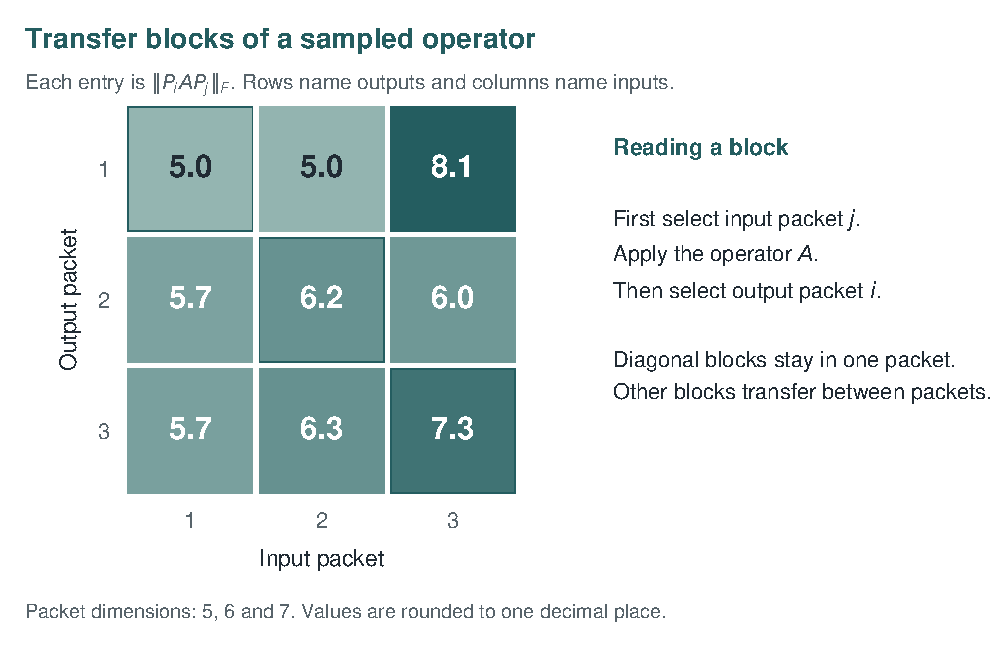
\includegraphics[width=0.96\textwidth]{02_transfer_block_norms.pdf}
\caption{An operator represented by the norms of its blocks between packets. The diagonal entries preserve packets. Entries outside the diagonal describe transfers between packets.}
\label{fig:transfer-blocks}
\end{figure}

\section{Transfer graphs and directed packet generation}



\begin{readerroadmap}
The transfer graph records which blocks between packets occur in a declared generating family.  Reachability constrains every word in that family.  To obtain an exact seed count from the graph, we also need hypotheses that let generation propagate along its edges.
\end{readerroadmap}
\subsection{Graphs generated by declared operators}

\begin{definition}[Transfer graph of a family generating the algebra]
\label{def:transfer-graph}
Let $\Pcal=(P_\alpha)_{\alpha\in I}$ be a finite packet system on $X$ with every $P_\alpha\in\A$.  Let $\mathcal G\subseteq\A$ satisfy
\[
\A=\alg_{\bbk}\bigl(\{P_\alpha:\alpha\in I\}\cup\mathcal G\bigr),
\]
where $\alg_{\bbk}(E)$ denotes the unital subalgebra over $\bbk$ generated by $E$.  The transfer graph $\Gamma(\mathcal G,\Pcal)$ has vertex set $I$ and an arrow
\[
\alpha\longrightarrow\beta
\]
when
\[
P_\beta GP_\alpha\neq0
\]
for at least one $G\in\mathcal G$.  Reachability includes paths of length zero.
\end{definition}
\RecordID{PSC-I-D-TRANSFER-GRAPH}

\begin{theorem}[Reachability support of the generated algebra]
\label{thm:algebra-reachability-support}
For every $A\in\A$,
\[
P_\beta AP_\alpha=0
\qquad\text{whenever }\beta\notin\Reach(\alpha).
\]
Equivalently,
\[
\A\subseteq\mathfrak M_{R_\Gamma},
\qquad
R_\Gamma:=\{(\beta,\alpha):\beta\in\Reach(\alpha)\}.
\]
\end{theorem}
\RecordID{PSC-I-T-ALGEBRA-REACHABILITY-SUPPORT}
\Depends{PSC-I-D-TRANSFER-GRAPH and PSC-I-C-BLOCK-POWERS.}

\begin{proof}
It is enough to treat a word in the generators and packet projectors.  Insert
\[
I=\sum_{\gamma\in I}P_\gamma
\]
between consecutive nonprojector generators.  Every resulting $(\beta,\alpha)$ block is a finite sum of products
\[
P_\beta G_mP_{\gamma_{m-1}}
G_{m-1}\cdots
P_{\gamma_1}G_1P_\alpha.
\]
A nonzero product requires every consecutive block to be nonzero, hence gives a directed path
\[
\alpha\to\gamma_1\to\cdots\to\gamma_{m-1}\to\beta.
\]
Packet projectors only insert stationary steps.  Thus a word has no block from $\alpha$ to an unreachable $\beta$.  Linear combinations preserve the same zero pattern.
\end{proof}

\begin{interpretation}
The graph belongs to the declared generating family within \(\End(X)\).  Multiplying its generators concatenates paths, so a word in them cannot create a block outside graph reachability.  Reachability alone gives less information in the other direction.  A nonzero edge block may reach only a proper subspace of its target packet.
\end{interpretation}


A path records a possible sequence of transfers.  It does not guarantee that the composed transfer is nonzero.  The image of one block may lie in the kernel of the next, and different path contributions may cancel when they are added.  The reachability theorem therefore gives a restriction on support.  To prove that a target packet is generated, we must also examine what the blocks do to vectors.  Surjectivity along edges will provide that additional information below.

\subsection{Reachability obstructions for seeds}
\begin{proposition}[Reachability obstruction for generated hulls]
\label{prop:reachability-obstruction}
Let $I_0\subseteq I$ and let
\[
S\subseteq\bigoplus_{\alpha\in I_0}X_\alpha.
\]
Then
\[
\boxed{
\Hull_{\A}(S)
\subseteq
\bigoplus_{\beta\in\Reach(I_0)}X_\beta.
}
\]
In particular, no seed supported outside a source strongly connected component can generate a nonzero vector in that source component.
\end{proposition}
\RecordID{PSC-I-P-REACHABILITY-OBSTRUCTION}
\Depends{PSC-I-T-ALGEBRA-REACHABILITY-SUPPORT.}

\begin{proof}
For $s\in S$, write $s=\sum_{\alpha\in I_0}P_\alpha s$.  If $\beta$ is unreachable from $I_0$, then for every $A\in\A$,
\[
P_\beta As
=
\sum_{\alpha\in I_0}P_\beta AP_\alpha s
=0
\]
by \cref{thm:algebra-reachability-support}.  The same holds for every finite linear combination of orbit vectors.
\end{proof}

\subsection{Packet pure generation and source components}
A strongly connected component groups packets that can reach one another.  The condensation graph replaces each such group by a single vertex.  It has no directed cycles between distinct components.  A source component has no incoming edge from another component, so generation there must begin with seed coordinates already present in that component.  The rank below records the effect of requiring each seed to lie in a single packet.

\Needspace{15\baselineskip}
\begin{definition}[Packet pure seed rank]
\label{def:directed-seed-rank}
A vector is packet pure when it is zero or lies in one packet space $X_\alpha$, equivalently when its packet support has cardinality at most one.  Define
\[
\psrank_{\A,\Pcal}(X)
:=
\min\{|S|:S\text{ is packet-pure and }\A S=X\}.
\]
For $C\subseteq I$, put
\[
P_C:=\sum_{\alpha\in C}P_\alpha,
\qquad
X_C:=P_CX,
\qquad
\A_C:=P_C\A P_C,
\]
and define the local packet pure rank
\[
r_C:=\psrank_{\A_C,\Pcal|_C}(X_C).
\]
\end{definition}
\RecordID{PSC-I-D-DIRECTED-SEED-RANK}

\begin{proposition}[Basic packet pure rank bounds]
\label{prop:packet-pure-rank-bounds}
For every $A$ module resolved into packets with $P_\alpha\in A$,
\[
\boxed{
\srank_A(X)
\leq
\psrank_{A,\Pcal}(X)
\leq
\sum_{\alpha\in I}
\srank_{P_\alpha A P_\alpha}(X_\alpha).
}
\]
The corner algebra on the right is unital on $X_\alpha$ with identity $P_\alpha$.
\end{proposition}
\RecordID{PSC-I-P-PACKET-PURE-RANK-BOUNDS}
\Depends{PSC-I-D-SEED-RANK and PSC-I-D-DIRECTED-SEED-RANK.}

\begin{proof}
Every packet pure generating family is an unrestricted generating family, which gives the first inequality.  For each $\alpha$, choose a minimal generating family $S_\alpha\subseteq X_\alpha$ for the corner action $P_\alpha A P_\alpha$.  The union $S=\bigcup_\alpha S_\alpha$ is packet pure.  Since every $x\in X$ has the unique decomposition $x=\sum_\alpha x_\alpha$ and every $x_\alpha$ lies in $(P_\alpha A P_\alpha)S_\alpha\subseteq AS$, the union generates $X$.  Its cardinality is at most the displayed sum.
\end{proof}

\begin{definition}[Packet system surjective along edges]
\label{def:edge-surjective}
The module resolved into packets is surjective along edges relative to $\Gamma(\mathcal G,\Pcal)$ when, for every graph edge $\alpha\to\beta$, there exists $B\in\A$ such that the pure block
\[
P_\beta BP_\alpha:X_\alpha\twoheadrightarrow X_\beta
\]
is surjective.
\end{definition}
\RecordID{PSC-I-D-EDGE-SURJECTIVE}

\begin{theorem}[Source component formula for packet pure seed rank]
\label{thm:source-component-rank}
Assume $I$ is finite, every packet space is nonzero, and the module resolved into packets is surjective along edges.  Let $\mathfrak C_0$ be the set of source strongly connected components of the condensation graph of $\Gamma(\mathcal G,\Pcal)$.  Then
\[
\boxed{
\psrank_{\A,\Pcal}(X)
=
\sum_{C\in\mathfrak C_0}r_C.
}
\]
\end{theorem}
\RecordID{PSC-I-T-SOURCE-COMPONENT-SEED-RANK}
\Depends{PSC-I-P-REACHABILITY-OBSTRUCTION and PSC-I-D-EDGE-SURJECTIVE.}
\Exports{Residual transport forests and directed source rank calculations.}

\begin{proof}
Let $S$ be a packet pure generating family for $X$.  Discard zero seeds, which do not change the generated hull, and fix a source component $C$.  Seeds outside $C$ cannot reach $C$ by \cref{prop:reachability-obstruction}.  Moreover, for $s\in X_C$ and $A\in\A$,
\[
P_CAs=(P_CAP_C)s\in\A_Cs.
\]
Thus the seeds of $S$ lying in $X_C$ must generate $X_C$ under $\A_C$, and there are at least $r_C$ of them.  Summing over disjoint source components gives
\[
\psrank_{\A,\Pcal}(X)
\geq
\sum_{C\in\mathfrak C_0}r_C.
\]

For the reverse inequality, choose for each source component $C$ a packet pure family $S_C$ of size $r_C$ generating $X_C$ under $\A_C$, and put $S=\bigcup_CS_C$.  Then every source component lies in $\A S$.  Traverse the finite condensation graph in a topological order.  Suppose all components preceding a component $D$ that is not a source have already been shown to lie in $\A S$.  Choose an incoming condensation edge from such a component to $D$, represented by a graph edge $\alpha\to\beta$ with $\alpha$ already generated and $\beta\in D$.  Surjectivity along edges gives a pure block
\[
B_{\beta\alpha}:X_\alpha\twoheadrightarrow X_\beta.
\]
Because $X_\alpha\subseteq\A S$ and $\A S$ is invariant under $\A$, surjectivity implies $X_\beta\subseteq\A S$.  For any other vertex $\gamma\in D$, choose a directed path inside the strongly connected component from $\beta$ to $\gamma$.  Successive surjective edge blocks propagate the full packet space along the path, so $X_\gamma\subseteq\A S$.  Hence $X_D\subseteq\A S$.  Induction over the condensation graph gives $X=\A S$, proving the upper bound.
\end{proof}

\begin{hypothesisguide}
The formula for source components uses local generation inside those components and surjectivity along the edges.  Local generation supplies the starting packet spaces.  Surjectivity then propagates their full spaces through the condensation graph.  Without it, a path may exist while its blocks reach only a proper subspace.
\end{hypothesisguide}


\begin{definition}[Packet propagating system]
\label{def:packet-propagating}
A packet system that is surjective along edges is called packet propagating when every packet space $X_\alpha$ is cyclic under its diagonal corner algebra
\[
P_\alpha\A P_\alpha.
\]
\end{definition}
\RecordID{PSC-I-D-PACKET-PROPAGATING}

\begin{corollary}[Unweighted source component count]
\label{cor:source-component-count}
Assume the module resolved into packets is packet propagating and $X_\alpha\neq0$ for every $\alpha\in I$.  If $c_0$ denotes the number of source strongly connected components, then
\[
\boxed{
\psrank_{\A,\Pcal}(X)=c_0.
}
\]
\end{corollary}
\RecordID{PSC-I-C-SOURCE-COMPONENT-COUNT}
\Depends{PSC-I-T-SOURCE-COMPONENT-SEED-RANK.}

\begin{proof}
Fix a source component $C$ and a vertex $\alpha\in C$.  Choose a cyclic vector $s\in X_\alpha$ for $P_\alpha\A P_\alpha$.  It generates all of $X_\alpha$.  Strong connectivity and surjectivity along edges then propagate the whole packet space to every vertex of $C$.  Thus $r_C=1$ for every source component.  Apply \cref{thm:source-component-rank}.
\end{proof}

\begin{boundary}[Mixed support seeds can merge source requirements]
\label{bnd:packet-pure-boundary}
The source component formulas concern packet pure seeds.  They do not give the unrestricted seed rank.  For example, let
\[
\A=\bbk\times\bbk,
\qquad
X=\bbk\oplus\bbk
\]
with the coordinate action and the two coordinate packet projectors.  The transfer graph has two source components and
\[
\psrank_{\A,\Pcal}(X)=2,
\]
but the mixed vector $(1,1)$ is cyclic, so
\[
\srank_{\A}(X)=1.
\]
\end{boundary}
\RecordID{PSC-I-B-PACKET-PURE-BOUNDARY}

\begin{microexample}[title={Why mixed seeds change the answer}]
Let the acting algebra be diagonal on \(X=X_1\oplus X_2\), with no transfer between the packets.  Generation by packet pure seeds requires one seed in each source component, so \(\psrank=2\).  A single mixed vector \(x_1+x_2\) may generate both packets of dimension one under the diagonal action, so unrestricted seed rank can be \(1\).
\end{microexample}

\begin{sectionrecap}
Graph reachability restricts which blocks can be nonzero in the algebra generated by the declared operators.  Source components give the exact rank for packet pure seeds under the stated local generation and edge propagation hypotheses.  Seeds with several nonzero packet coordinates have a different minimum count and may meet several source requirements at once.
\end{sectionrecap}



\section{Coordinate transport, morphisms, invariant exact sequences, and completion}
\begin{readerroadmap}
This section follows packet data through changes of coordinates, maps between systems, and passage to a quotient.  It then explains the additional assumptions needed when density, topology, or completion enters the argument.
\end{readerroadmap}
\subsection{Coordinate changes and packet compatible morphisms}

\begin{theorem}[Coordinate transport]
\label{thm:coordinate-transport}
Let $U:X\to Y$ be a vector space isomorphism and let $\Pcal=(P_\alpha)$ be a packet system on $X$.  Define
\[
Q_\alpha:=UP_\alpha U^{-1}.
\]
Then $\Qcal=(Q_\alpha)$ is a packet system on $Y$.  For $\widetilde T=UTU^{-1}$,
\[
\boxed{
Q_\beta\widetilde TQ_\alpha
=
U(P_\beta TP_\alpha)U^{-1}.
}
\]
Hence packet dimensions, zero patterns, and support preorders are invariant under coordinate transport.  If a declared algebra generating family $\mathcal G$ is transported to $U\mathcal G U^{-1}$, then its transfer graph and reachability relation are also preserved.
\end{theorem}
\RecordID{PSC-I-T-COORDINATE-TRANSPORT}
\Depends{PSC-I-D-PACKET-SYSTEM and PSC-I-D-TRANSFER-BLOCK.}

\begin{proof}
Conjugation preserves products and sums, so
\[
Q_\alpha Q_\beta
=UP_\alpha P_\beta U^{-1}
=\delta_{\alpha\beta}Q_\alpha,
\qquad
\sum_\alpha Q_\alpha=I_Y.
\]
The block identity is direct multiplication:
\[
Q_\beta\widetilde TQ_\alpha
=UP_\beta TP_\alpha U^{-1}.
\]
All listed invariants are determined by these transported blocks.
\end{proof}

\begin{interpretation}
An isomorphism changes the coordinates of each packet while preserving the direct sum structure.  Conjugating the projectors and the operator together preserves every block identity.  This is the linear prototype for the gauge changes used later in the series.
\end{interpretation}


\begin{definition}[Packet compatible operator morphism]
\label{def:packet-morphism}
Let $(X,\A,\Pcal)$ and $(Y,\B,\Qcal)$ be packet resolved operator modules with packet index sets $I$ and $J$.  A packet compatible operator morphism is a triple
\[
(\Phi,\varphi,\sigma)
\]
consisting of a unital algebra homomorphism $\varphi:\A\to\B$, a linear map $\Phi:X\to Y$ satisfying
\[
\Phi(Ax)=\varphi(A)\Phi(x),
\]
and a map $\sigma:I\to J$ satisfying
\[
Q_j\Phi
=
\Phi P_{\sigma^{-1}(j)},
\qquad
P_{\sigma^{-1}(j)}:=
\sum_{\sigma(\alpha)=j}P_\alpha.
\]
An empty fiber is interpreted as the zero projector.
\end{definition}
\RecordID{PSC-I-D-PACKET-MORPHISM}

The packet index map records which source packets are grouped into each target packet.  Its compatibility equation says that projecting after transport gives the same result as first collecting those source packets.  The intertwining equation separately ensures that the declared operator actions agree with the transport.  Both conditions matter when comparing transfer blocks.

\begin{definition}[Morphism of seeded systems]
\label{def:seed-morphism}
A morphism
\[
(X,\A,S,\Pcal)\longrightarrow(Y,\B,S',\Qcal)
\]
is a packet compatible operator morphism satisfying the seed condition
\[
\Phi(S)\subseteq\Hull_{\B}(S').
\]
In the topological category all maps and actions are required to be continuous and the seed condition uses the topological hull when declared.
\end{definition}
\RecordID{PSC-I-D-SEED-MORPHISM}

\begin{theorem}[Naturality of generated hulls and transfer blocks]
\label{thm:naturality}
Let $(\Phi,\varphi,\sigma)$ be a packet compatible operator morphism.  For every subset $S\subseteq X$,
\[
\boxed{
\Phi(\Hull_{\A}(S))
=
\Hull_{\varphi(\A)}(\Phi(S))
\subseteq
\Hull_{\B}(\Phi(S)).
}
\]
For $T\in\A$ and $i,j\in J$,
\[
\boxed{
Q_j\varphi(T)Q_i\Phi
=
\sum_{\substack{\sigma(\beta)=j\\\sigma(\alpha)=i}}
\Phi P_\beta TP_\alpha.
}
\]
If $\Phi$ is surjective and $S$ generates $X$, then $\Phi(S)$ generates $Y$ under $\varphi(\A)$ and hence under $\B$.  If, in addition, the morphism is seeded, then $S'$ generates $Y$.
\end{theorem}
\RecordID{PSC-I-T-NATURALITY}
\Depends{PSC-I-D-PACKET-MORPHISM and PSC-I-T-BLOCK-MULTIPLICATION.}
\Exports{The canonical naturality theorem for every later realization.}

\begin{proof}
Every element of $\Phi(\Hull_{\A}(S))$ is a finite sum of vectors
\[
\Phi(As)=\varphi(A)\Phi(s),
\]
so it belongs to $\Hull_{\varphi(\A)}(\Phi(S))$.  Conversely, every generator $\varphi(A)\Phi(s)$ equals $\Phi(As)$, giving equality.

For the block formula, use intertwining and packet compatibility twice:
\begin{align*}
Q_j\varphi(T)Q_i\Phi
&=Q_j\varphi(T)\Phi P_{\sigma^{-1}(i)}\\
&=Q_j\Phi TP_{\sigma^{-1}(i)}\\
&=\Phi P_{\sigma^{-1}(j)}TP_{\sigma^{-1}(i)}\\
&=\sum_{\substack{\sigma(\beta)=j\\\sigma(\alpha)=i}}
\Phi P_\beta TP_\alpha.
\end{align*}
If $\Phi$ is surjective and $\Hull_{\A}(S)=X$, the hull equality gives $Y=\Hull_{\varphi(\A)}(\Phi(S))$.  If $\Phi(S)\subseteq\Hull_{\B}(S')$, then $\Hull_{\B}(\Phi(S))\subseteq\Hull_{\B}(S')$, so $S'$ generates $Y$.
\end{proof}

\begin{keyidea}
Naturality gives two ways to compute the same transported block.  One may apply the target operator between target projectors, or sum the source blocks whose packet indices map to those target indices and then apply the morphism.  The theorem also identifies the image of the generated hull.  These equalities make the comparison between the two systems precise.
\end{keyidea}


\begin{proposition}[Category of seeded packet systems]
\label{prop:seed-category}
Packet compatible operator morphisms compose, seeded morphisms compose, and identity morphisms satisfy both definitions.  Thus packet resolved operator modules form a category $\mathbf{PktMod}$ and seeded packet systems form a category $\mathbf{SeedSys}$.
\end{proposition}
\RecordID{PSC-I-P-SEED-SYSTEM-CATEGORY}
\Depends{\nolinkurl{PSC-I-D-PACKET-MORPHISM},
\nolinkurl{PSC-I-D-SEED-MORPHISM}, and
\nolinkurl{PSC-I-T-NATURALITY}.}

\begin{proof}
Let $(\Phi,\varphi,\sigma):(X,\A,\Pcal)\to(Y,\B,\Qcal)$ and $(\Psi,\psi,\tau):(Y,\B,\Qcal)\to(Z,\Ccal,\Rcal)$ be morphisms.  Intertwining is preserved because
\[
\Psi\Phi(Ax)
=
\Psi(\varphi(A)\Phi x)
=
(\psi\circ\varphi)(A)\Psi\Phi x.
\]
For $k$ in the target packet set,
\begin{align*}
R_k\Psi\Phi
&=\Psi Q_{\tau^{-1}(k)}\Phi\\
&=\Psi\Phi
\sum_{\tau(\sigma(\alpha))=k}P_\alpha.
\end{align*}
Thus the composite packet map is $\tau\circ\sigma$.  If the morphisms are seeded, then
\[
\Phi(S)\subseteq\Hull_{\B}(S'),
\qquad
\Psi(S')\subseteq\Hull_{\Ccal}(S'').
\]
By \cref{thm:naturality},
\[
\Psi\Phi(S)
\subseteq
\Psi(\Hull_{\B}(S'))
\subseteq
\Hull_{\Ccal}(\Psi(S'))
\subseteq
\Hull_{\Ccal}(S'').
\]
Identity maps satisfy the definitions with identity algebra and packet maps.
\end{proof}

\subsection{Invariant subspaces and quotient packets}
Passage to a quotient uses two separate invariance assumptions.  The packet projectors must preserve the subspace for packet coordinates to descend.  An operator must also preserve that subspace for its action, and hence its transfer blocks, to descend.  The first condition is enough for the packet exact sequence.  The second enters the corollary about transfer blocks.

\begin{theorem}[Packet exact sequence for an invariant subspace]
\label{thm:packet-exact-sequence}
Let $K\leq X$ satisfy $P_\alpha K\subseteq K$ for every $\alpha$.  Define
\[
K_\alpha:=P_\alpha K=K\cap X_\alpha
\]
and
\[
\overline P_\alpha(x+K):=P_\alpha x+K.
\]
Then:
\begin{enumerate}[label=(\roman*)]
\item The nonzero restrictions $P_\alpha|_K$ form a packet system on $K$.
\item The nonzero $\overline P_\alpha$ form a packet system on $X/K$.
\item For every $\alpha$ there is a short exact sequence
\[
0\longrightarrow K_\alpha
\longrightarrow X_\alpha
\longrightarrow \overline P_\alpha(X/K)
\longrightarrow0,
\]
and
\[
\overline P_\alpha(X/K)
\cong
X_\alpha/(X_\alpha\cap K)
\cong
(X_\alpha+K)/K.
\]
\item The full exact sequence decomposes packetwise as the direct sum of these short exact sequences.
\end{enumerate}
\end{theorem}
\RecordID{PSC-I-T-PACKET-EXACT-SEQUENCE}
\Depends{PSC-I-T-EXACT-PACKET-COORDINATES.}
\Exports{Packetwise subobject and quotient constructions.}

\begin{proof}
Restriction preserves idempotency, pairwise annihilation, and the identity sum on $K$.  If $x\in K\cap X_\alpha$, then $x=P_\alpha x\in P_\alpha K$, proving $K_\alpha=K\cap X_\alpha$.

The quotient operator is well defined because replacing $x$ by $x+k$ changes $P_\alpha x$ by $P_\alpha k\in K$.  The idempotent and annihilation identities descend, and the sum is the identity on $X/K$.  The map $X_\alpha\to X/K$ has image $(X_\alpha+K)/K$ and kernel $X_\alpha\cap K$, giving the short exact sequence and the quotient isomorphisms.  Exact packet coordinates identify the original sequence with the direct sum over $\alpha$.
\end{proof}

\begin{microexample}[title={Packet descent to a quotient}]
Let \(X=X_1\oplus X_2\) and let \(K\subseteq X_1\) be a subspace.  The quotient has packets \(X_1/K\) and \(X_2\).  Any operator preserving \(K\) descends with the same organization by source and target packets, with blocks entering or leaving the first packet replaced by their induced quotient maps.  An induced block can become zero even when its original block is nonzero, so the pattern of nonzero blocks can shrink.  Any resulting zero packet is removed from the quotient packet system.
\end{microexample}


\begin{theorem}[Packet descent through an invariant quotient]
\label{thm:quotient-packet-descent}
Under the hypotheses of \cref{thm:packet-exact-sequence}, the operators
\[
\overline P_\alpha(x+K)=P_\alpha x+K
\]
are well defined pairwise annihilating idempotents with sum $I_{X/K}$, and the quotient map satisfies
\[
\boxed{\pi P_\alpha=\overline P_\alpha\pi.}
\]
After zero packets are removed, they form the canonical quotient packet system.
\end{theorem}
\RecordID{PSC-I-T-QUOTIENT-PACKET-DESCENT}
\Depends{PSC-I-T-PACKET-EXACT-SEQUENCE.}

\begin{proof}
All assertions are the quotient part of \cref{thm:packet-exact-sequence}.  The intertwining identity follows directly from the definition:
\[
\overline P_\alpha\pi(x)=P_\alpha x+K=\pi P_\alpha(x).
\]
\end{proof}

\begin{corollary}[Restriction and quotient of transfer blocks]
\label{cor:block-descent}
Under the hypotheses of \cref{thm:packet-exact-sequence}, let $T\in\End(X)$ preserve $K$.  Then every block $T_{\beta\alpha}$ maps $K_\alpha$ into $K_\beta$, and the induced quotient operator $\overline T$ satisfies
\[
\boxed{
\overline T_{\beta\alpha}\,\pi
=
\pi T_{\beta\alpha},
}
\]
where $\pi:X\twoheadrightarrow X/K$.
\end{corollary}
\RecordID{PSC-I-C-QUOTIENT-PACKET-DESCENT}
\Depends{PSC-I-T-PACKET-EXACT-SEQUENCE.}

\begin{proof}
If $x\in K_\alpha$, then $Tx\in K$, so
\[
T_{\beta\alpha}x=P_\beta Tx\in K\cap X_\beta=K_\beta.
\]
On the quotient,
\[
\overline T_{\beta\alpha}\pi
=
\overline P_\beta\overline T\overline P_\alpha\pi
=
\pi P_\beta TP_\alpha.
\]
\end{proof}

\begin{corollary}[Topological packet exact sequence]
\label{cor:topological-packet-exact-sequence}
If $X$ is Banach, the $P_\alpha$ are bounded, and $K$ is closed and packet invariant, then every packet sequence in \cref{thm:packet-exact-sequence} is a short exact sequence of Banach spaces with bounded maps, and the quotient projectors are bounded.
\end{corollary}
\RecordID{PSC-I-C-TOPOLOGICAL-PACKET-EXACT-SEQUENCE}
\Depends{\nolinkurl{PSC-I-T-PACKET-EXACT-SEQUENCE} and
\nolinkurl{PSC-I-T-BANACH-PACKET-ISOMORPHISM}.}

\begin{proof}
Closedness of $K$ makes $X/K$ Banach.  The restricted projectors are bounded, and the quotient projectors are bounded because
\[
\|\overline P_\alpha(x+K)\|_{X/K}
\leq
\|P_\alpha\|\,\|x+K\|_{X/K}.
\]
The packet spaces are closed ranges of bounded idempotents.
\end{proof}

\subsection{Dense images, quotient topology, and completion}
Algebraic generation uses finite linear combinations of operator images.  Topological generation allows limits of those combinations in the declared topology.  A continuous surjection carries this approximation property to the target, but identifying the target with a topological quotient requires a further assumption.

\begin{theorem}[Dense realization theorem]
\label{thm:dense-realization}
Let $X$ and $Y$ be Hausdorff topological vector spaces, let $\Phi:X\to Y$ be continuous, surjective, and intertwining with respect to $\varphi$, and let $S$ topologically generate $X$.  Then $\Phi(S)$ topologically generates $Y$.  If finite continuous packet systems satisfy
\[
Q_j\Phi=\Phi P_{\sigma^{-1}(j)},
\]
then
\[
\boxed{
Q_jY=\Phi(P_{\sigma^{-1}(j)}X)
}
\]
for every $j$.
\end{theorem}
\RecordID{PSC-I-T-DENSE-REALIZATION}
\Depends{PSC-I-T-NATURALITY.}

\begin{proof}
Given $y=\Phi(x)$, choose a net $x_\lambda\in\Hull_{\A}(S)$ converging to $x$.  Then
\[
\Phi(x_\lambda)\to y,
\]
and naturality places every $\Phi(x_\lambda)$ in $\Hull_{\B}(\Phi(S))$.  Hence the latter hull is dense.  For packets, one inclusion follows from compatibility.  Conversely, if $y=Q_jy$, choose $x$ with $\Phi(x)=y$.  Then
\[
y=Q_j\Phi(x)=\Phi P_{\sigma^{-1}(j)}x.
\]
\end{proof}

\begin{theorem}[Quotient topology and completed realization]
\label{thm:quotient-topology}
Let $\Phi:X\twoheadrightarrow Y$ be a continuous linear quotient map between Hausdorff topological vector spaces, and put $K=\Ker\Phi$.  Then the induced map
\[
\widetilde\Phi:X/K\longrightarrow Y
\]
is a topological isomorphism.  If $D\subseteq X$ is a linear subspace whose image $\Phi(D)$ is dense in a complete space $Y$, then the completion of
\[
D/(D\cap K)
\]
in the topology transported from $Y$ is canonically isomorphic to $Y$.
\end{theorem}
\RecordID{PSC-I-T-QUOTIENT-TOPOLOGY-COMPLETION}
\Depends{PSC-I-T-COMPLETED-PRESENTATION, the definition of quotient topology, and uniqueness of completion.}

\begin{proof}
The algebraic first isomorphism theorem gives a bijection $\widetilde\Phi$.  By definition of the quotient topology, a set $U\subseteq X/K$ is open exactly when its preimage in $X$ is open.  Because $\Phi$ is a quotient map, this is equivalent to $\widetilde\Phi(U)$ being open in $Y$.  Thus $\widetilde\Phi$ is a homeomorphism.  The second statement applies the dense completion argument of \cref{thm:completed-presentation} to the injective map $D/(D\cap K)\to Y$.
\end{proof}

\begin{boundary}[Continuous surjections and quotient topology]
\label{bnd:topological-quotient}
Continuity and surjectivity transport density as in \cref{thm:dense-realization}.  They do not by themselves identify the given topology on $Y$ with the quotient topology from $X$.  The stronger conclusion in \cref{thm:quotient-topology} requires the quotient map hypothesis or an equivalent open mapping condition.
\end{boundary}
\RecordID{PSC-I-B-TOPOLOGICAL-QUOTIENT}

\begin{warningbox}
A continuous surjective linear map need not be a quotient map in arbitrary topological vector spaces.  The algebraic first isomorphism theorem gives a bijection on the quotient.  A topological isomorphism requires the quotient topology to agree with the target topology.  An applicable open mapping theorem can supply this agreement, as it does for continuous linear surjections between Banach spaces.
\end{warningbox}

The completion statement uses the topology transported from the target space.  This choice ensures that approximation in the quotient means approximation in the target.  A topology inherited from the original subspace need not give the same completion unless the two topologies agree.  The theorem therefore names the topology as part of its conclusion.

\begin{sectionrecap}
Packet systems transport by conjugation, form a category under packet compatible seeded morphisms, restrict to invariant subspaces, descend to invariant quotients, and survive completion under explicit boundedness and quotient topology hypotheses.
\end{sectionrecap}


\begin{figure}[htbp]
\centering
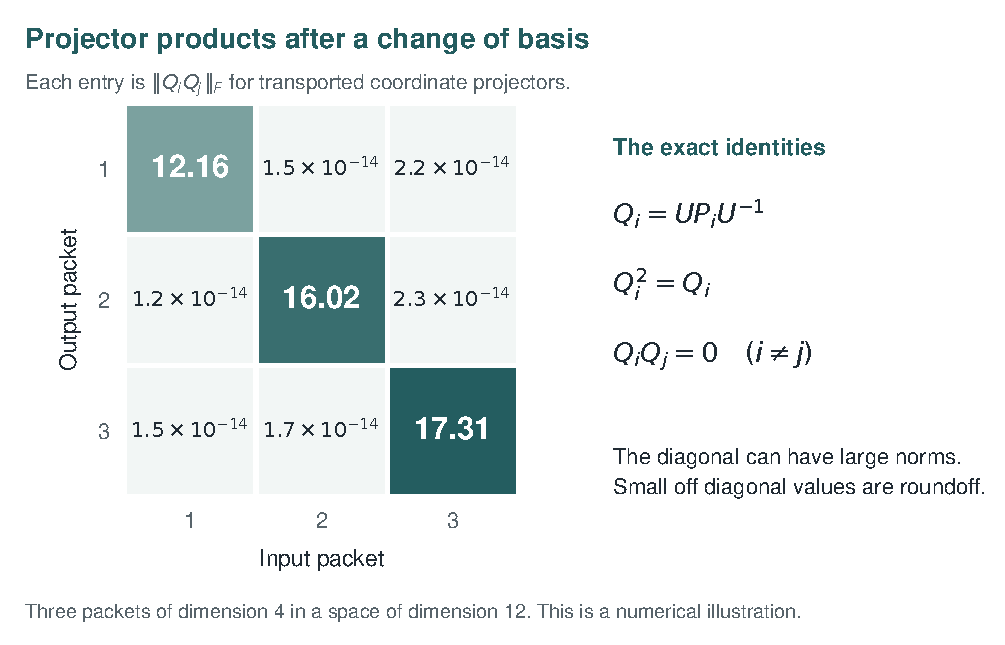
\includegraphics[width=0.96\textwidth]{09_coordinate_transport.pdf}
\caption{Numerical certificate for a nonorthogonal transported packet system. The diagonal products retain idempotent size while off diagonal products remain at roundoff level.}
\label{fig:coordinate-transport}
\end{figure}

\section{Realization functors and semantic theorem transport}
\begin{readerroadmap}
A later domain is a genuine realization only when the relevant structures and identities are preserved.  The purpose of this section is to replace informal analogy by a precise preservation profile.
\end{readerroadmap}
\subsection{Preservation profiles}

\begin{definition}[Realization functor and preservation profile]
\label{def:realization-functor}
Let $\mathbf{SeedSys}_{\mathrm{abs}}$ be an abstract category of seed systems and let $\mathbf C_D$ be a domain category.  A realization functor is a functor
\[
\mathsf{Ev}_D:\mathbf{SeedSys}_{\mathrm{abs}}\longrightarrow\mathbf C_D
\]
with a declared preservation profile specifying which of the following structures are preserved:
\[
\begin{gathered}
0,\ I,\ \text{finite sums},\ \text{composition},\ \text{biproducts},\\
\text{kernels},\ \text{cokernels},\ \text{quotients},\ \text{tensor products},\\
\text{packet idempotents},\ \text{transfer blocks},\ \text{topological completions}.
\end{gathered}
\]
Preservation of a structure means preservation of its defining identity or universal property, not merely a similarity of notation.
\end{definition}
\RecordID{PSC-I-D-REALIZATION-FUNCTOR}

\begin{theorem}[Equational realization principle]
\label{thm:realization-export}
Let $F:\mathbf C\to\mathbf D$ be an additive functor between preadditive categories.  Any equality of morphisms constructed from declared generating morphisms by finite sums, additive inverses, identities, zero maps, and composition is preserved by $F$.  Scalar multiplication by a coefficient ring is also preserved when the categories are enriched over that ring and $F$ is linear for the declared enrichment.  If a proof additionally uses a chosen biproduct, kernel, cokernel, quotient, tensor product, or completion and $F$ preserves that construction in its declared profile, then the corresponding proof diagram is transported to $\mathbf D$.
\end{theorem}
\RecordID{PSC-I-T-REALIZATION-EXPORT}
\Depends{PSC-I-D-REALIZATION-FUNCTOR.}
\Exports{The formal criterion for semantic transfer across domains.}

\begin{proof}
Functoriality gives
\[
F(I)=I,
\qquad
F(g\circ f)=F(g)\circ F(f),
\]
and additivity gives
\[
F(0)=0,
\qquad
F(f+g)=F(f)+F(g),
\qquad
F(-f)=-F(f).
\]
If the declared enrichment is present, linearity additionally gives $F(af)=aF(f)$ for every coefficient $a$.  A structural induction on the construction of a morphism expression therefore carries every permitted equational proof to its image under $F$.  If a step invokes a universal construction, preservation means that the image diagram satisfies the same universal property.  The uniquely induced morphism in the source proof is therefore carried to the uniquely induced morphism in the target proof.  Repeating this argument through the finite proof diagram transports the conclusion.
\end{proof}

\begin{interpretation}
The equational principle covers identities built from operations the functor preserves.  Additive identities require additivity.  Identities with scalar coefficients require linear enrichment.  Quotients, tensor products, completions, kernels, or limits require their own preservation assumptions.  The preservation profile records the assumptions needed to carry each step of the proof into the target category.
\end{interpretation}


\subsection{From equation transport to semantic realization}
\begin{proposition}[Realization export principle]
\label{prop:realization-export}
Every canonical Chapter I identity whose proof uses only the operations listed in a realization functor's verified preservation profile remains valid after applying that functor.  If the proof uses a domain specific hypothesis not encoded by the functor, that hypothesis must be verified separately before the transported statement is promoted to a theorem.
\end{proposition}
\RecordID{PSC-I-P-REALIZATION-EXPORT}
\Depends{PSC-I-T-REALIZATION-EXPORT.}

\begin{proof}
The first assertion is \cref{thm:realization-export}.  The second is a logical boundary: a functor transports established identities and preserved universal constructions, but it does not create an unverified analytic, topological, positivity, finiteness, or integrality hypothesis.
\end{proof}

\begin{definition}[Semantic realization criterion]
\label{def:semantic-realization}
A domain theorem is a semantic realization of a canonical seed calculus theorem only when:
\begin{enumerate}[label=(\roman*)]
\item An explicit realization functor or intertwining construction is given.
\item The preservation profile covers every construction used in the canonical proof.
\item Every additional analytic, finiteness, convergence, positivity, or integrality hypothesis is verified in the domain.
\item The resulting conclusion is stated in the domain's native objects.
\end{enumerate}
Reuse of the words ``seed'', ``packet'', or ``transfer'' without these data is only syntactic reuse.
\end{definition}
\RecordID{PSC-I-D-SEMANTIC-REALIZATION}

\begin{warningbox}
A change of nouns is not a realization theorem.  Calling a frequency band, a ramification sector, and a symmetry sector a ``packet'' is only terminology until one exhibits the idempotents, proves reconstruction, identifies the transfer blocks, and checks that the relevant morphisms or limits preserve those structures.
\end{warningbox}

\begin{sectionrecap}
The preservation profile determines which equations and proof constructions pass to a new domain.  Checking it gives later chapters a concrete test for transporting a theorem: identify the realization, check each operation used in the proof, and verify the additional domain hypotheses.
\end{sectionrecap}


\section{Canonical export interface and claim boundary}
\begin{readerroadmap}
The export interface lets later chapters use the foundational proofs directly.  Each chapter can cite the stable record ID, state its domain hypotheses, and prove the new step specific to its realization.
\end{readerroadmap}

\begin{definition}[Worked realization interface]
\label{def:reserved-example-slots}
The foundational calculus is illustrated by four canonical algebraic realizations:
\begin{enumerate}[label=(\roman*)]
\item A typed quiver reachability model.
\item An algebraic coordinate ring presentation.
\item A companion and repeated primary single operator model.
\item Path and cycle adjacency models.
\end{enumerate}
The worked model sections below instantiate these four interfaces. A bilateral shift example records the analytic completion mechanism also used in Chapter V. Computational specifications connect the proofs with the verification companion and are not premises of the foundational theorems.
\end{definition}
\RecordID{PSC-I-ALG-EXAMPLE-SLOTS}

\begin{definition}[Chapter I export object]
\label{def:paper-one-export}
The canonical Chapter I export is
\[
\boxed{
\mathsf{PSC}_I=
\left(
\begin{array}{c}
\text{typed grammars and realized operator algebras},\\
\text{seed systems, free presentations, and seed rank},\\
\text{module-top, semisimple, and single-operator formulas},\\
\text{finite and unconditional packet coordinates},\\
\text{transfer blocks and support algebras},\\
\text{reachability and packet-pure source generation},\\
\text{morphisms, invariant exact sequences, quotients, completions},\\
\text{realization functors and equational theorem transport}
\end{array}
\right).
}
\]
\end{definition}
\RecordID{PSC-I-EXPORT}



\subsection{Use across chapters}
\begin{center}
\begin{longtable}{@{}>{\raggedright\arraybackslash}p{0.26\textwidth}>{\raggedright\arraybackslash}p{0.18\textwidth}>{\raggedright\arraybackslash}p{0.49\textwidth}@{}}
\toprule
\textbf{Chapter I export} & \textbf{Primary users} & \textbf{Later role}\\
\midrule
\endhead
Typed grammar and module equivalence & II to XII & Gives each domain a legal operator syntax and a concrete module realization.\\
Free seed presentation & IV, IX, X & Converts generated families into quotient presentations and relation modules.\\
Jacobson top seed rank & VII, X, XII & Computes minimal generators from semisimple multiplicity data.\\
Single operator formula & IV, VI, IX & Resolves recurrence, companion, and spectral chain generator counts.\\
Exact packet coordinates & II to XII & Supplies analysis, synthesis, and packetwise equality.\\
Tensor and dual packet systems & V, VII, VIII, XI & Controls product systems, observables, and paired representations.\\
Transfer block multiplication & II to XII & Converts operator composition into sums over packet paths.\\
Block intertwining equations & III, VII, XI & Expresses global equivalence or gluing as local packet equations.\\
Support preorder algebra & II, VIII, X & Produces triangular transfer structure and nilpotent strict transfer ideals.\\
Source component seed rank & VIII, X & Identifies the packet pure source requirements under propagation hypotheses.\\
Packet exact sequences and quotient descent & III, VI, X, XII & Carries packets through constraints, reductions, and deformation quotients.\\
Semantic realization criterion & IV to XII & Specifies when a domain theorem is a true realization of the common calculus.\\
\bottomrule
\end{longtable}
\end{center}


\begin{boundary}[Exact limits of Chapter I]
\label{bnd:final-claim-boundary}
The existence of an exact packet decomposition does not imply that the decomposition is computationally discoverable, numerically well conditioned, statistically identifiable, dynamically invariant, or mathematically useful.  The condition number in \cref{def:packet-condition-number} quantifies only coordinate stability once the packets are supplied.  Refinement towers, filtered transfer, nonlinear obstruction objects, automatic packet recovery, continuum limits, arithmetic lifts, and automorphic occupancy require additional theorems in later chapters.
\end{boundary}
\RecordID{PSC-I-B-FINAL-CLAIM-BOUNDARY}




\section{A typed quiver model}

A small quiver model shows how the path algebra records a direction that the available seeds cannot reach.

Let the quiver have vertices $U,V$ and arrows
\[
R:U\to U,
\qquad
A:U\to V,
\qquad
B:V\to U,
\]
with the relation in the path algebra
\[
BA=e_U,
\]
whose realization is the operator identity $BA=I_U$.
Realize
\[
U=\bbk^2,
\qquad
V=\bbk^3,
\]
by
\[
R=
\begin{pmatrix}0&-1\\1&0\end{pmatrix},
\qquad
A(u_1,u_2)=(u_1,u_2,0),
\qquad
B(v_1,v_2,v_3)=(v_1,v_2).
\]
Starting from the seed $e_1\in U$, repeated application of $R$ spans $U$, and $A$ carries that span onto the first two coordinates of $V$. Any path from $U$ to $V$ ends with $A$ and therefore lands in $\im A$. The third coordinate direction, which spans $\ker B$, is unreachable from a seed supported only at $U$. Therefore the generated representation is
\[
U\oplus\Span\{(1,0,0),(0,1,0)\}
\subsetneq U\oplus V.
\]
Adding the seed $(0,0,1)\in V$ generates the full representation.

\begin{proposition}[Typed reachability certificate]
\label{prop:typed-reachability}
In the preceding quiver realization, no seed supported at $U$ can generate the full representation, whereas the two seeds
\[
e_1\in U,
\qquad
e_3\in V
\]
do generate it.
\end{proposition}

\begin{proof}
The first claim follows because every path that starts at $U$ and ends in $V$ has final arrow $A$, so its image lies in $\im A$. For the second, $e_1$ and $Re_1$ span $U$. Their images under $A$ span $\im A$, and $e_3$ spans $\ker B$, the missing complementary direction in $V$.
\end{proof}

This example shows why a typed grammar is more than a notational convenience. The obstruction lies in the subspace $\ker B\subset V$, which is unreachable from seeds supported at $U$, and is visible before any coordinate calculation.

The arrow from one vertex to another records which type can be reached. Its image records which directions can be reached within that type. Here the first seed reaches both vertices, yet misses one direction at the second vertex. The extra seed supplies that direction directly. This is why reachability of a vertex alone does not settle generation of its entire space.

\section{Worked algebraic model: an elliptic coordinate ring}

Let $\operatorname{char}\bbk\ne2$ and let
\[
A=\bbk[x,y]/(y^2-x^3+x).
\]
The affine equation $y^2=x^3-x$ has classical discriminant $64$, which is nonzero under this hypothesis. Standard algebraic geometry then identifies its smooth projective completion as an elliptic curve \cite{silverman2009}. The Lean development checks the algebraic implication $2\ne0\Rightarrow64\ne0$, the quotient normal form, and the operator identities below. It does not formalize projective smoothness, genus, or the geometric identification of the discriminant. The packet computation itself uses only the displayed relation in the quotient ring.
Every class has a unique normal form
\[
f(x,y)=a(x)+y b(x).
\]
Indeed, $y^2-(x^3-x)$ is monic of degree two in $y$, so division in $\bbk[x][y]$ gives a unique remainder of degree less than two in $y$. Concretely, every power $y^m$ with $m\ge2$ can be reduced using
\[
y^2=x^3-x.
\]

\subsection{One module seed and two address operators}

Take the seed
\[
s=1
\]
and let $M_x,M_y$ be multiplication by $x$ and $y$. Then
\[
M_x^iM_y^js=x^iy^j,
\]
so the algebra, regarded as a module over its multiplication algebra, is generated by one seed.

The two packet spaces are
\[
A_0=\bbk[x],
\qquad
A_1=y\bbk[x].
\]
Let
\[
P_0(a+yb)=a,
\qquad
P_1(a+yb)=yb.
\]
These idempotents are linear over $\bbk$, annihilate one another, and satisfy $P_0+P_1=I$. They are not module maps over $A$, because multiplication by $y$ exchanges the two packets.

Identify the packet coefficients by
\[
A_0\oplus A_1\longrightarrow\bbk[x]\oplus\bbk[x],
\qquad
(a,yb)\longmapsto(a,b).
\]
In these ordered coefficient coordinates, with $M_x$ and $M_{x^3-x}$ denoting multiplication on $\bbk[x]$,
\[
{
M_x=
\begin{pmatrix}
M_x&0\\
0&M_x
\end{pmatrix},
\qquad
M_y=
\begin{pmatrix}
0&M_{x^3-x}\\
I&0
\end{pmatrix}.
}
\]
The two rows of the second matrix record the outgoing packet coefficients. An even input enters the odd packet without an additional factor. An odd input returns to the even packet through the factor imposed by the curve equation. Applying the matrix twice therefore preserves each packet and multiplies its coefficient by that factor.

The relation is reconstructed as an operator identity:
\[
M_y^2=M_x^3-M_x.
\]

\begin{figure}[htbp]
\centering
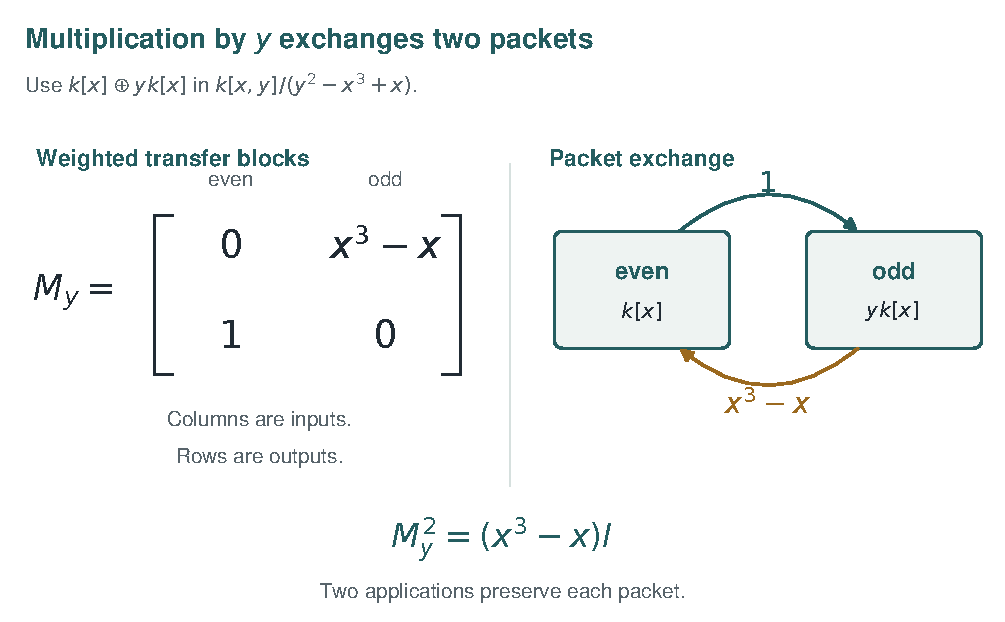
\includegraphics[width=0.96\textwidth]{08_elliptic_packet_transfer.pdf}
\caption{Multiplication by $y$ exchanges the even and odd packets. The transfer from the odd packet to the even packet carries the relation weight $x^3-x$.}
\label{fig:elliptic-transfer}
\end{figure}

\subsection{Exact product law}

Write
\[
f=a_0+ya_1,
\qquad
g=b_0+yb_1.
\]
Then
\[
{
fg
=
\bigl(a_0b_0+(x^3-x)a_1b_1\bigr)
+
y\bigl(a_0b_1+a_1b_0\bigr).
}
\]
This is a convolution law for the two packets. It is already visible at the linear operator level because multiplication by a fixed element is a transfer operator. The even output collects the product of the two even coefficients and the weighted product of the two odd coefficients. The odd output collects the two products with one even and one odd coefficient. The quotient relation is thus retained in the weight rather than discarded during the decomposition.

\begin{example}[Worked reduction]
Take
\[
f=x^2+y,
\qquad
g=x-y.
\]
Then
\[
\begin{aligned}
fg
&=x^3-x^2y+xy-y^2\\
&=x^3-x^2y+xy-(x^3-x)\\
&=x+(x-x^2)y.
\end{aligned}
\]
Thus
\[
P_0(fg)=x,
\qquad
P_1(fg)=(x-x^2)y.
\]
The symbolic certificate in the companion code performs the same quotient reduction exactly.
\end{example}

\subsection{What this example establishes}

The coordinate ring illustrates four distinct parts of the calculus:
\begin{enumerate}[label=(\roman*)]
\item the unit is a module seed.
\item $M_x$ and $M_y$ are address operators.
\item the curve equation is an operator relation.
\item parity in $y$ gives exact packet analysis, transfer, and reconstruction.
\end{enumerate}
It does not imply that every algebra can be presented as an algebra generated by one element. It shows instead that unital algebras are cyclic as modules over their full multiplication algebra.

\section{Worked signal model: a bilateral shift}

Let $\mathbb{F}\in\{\R,\C\}$ and let
\[
X=\ell^2(\Z;\mathbb F)
\]
with a family of bounded reindexing operators indexed by the integers
\[
(S_mx)[n]=x[n-m]
\qquad(m,n\in\Z).
\]
Thus $S_0=I$, $S_{m+r}=S_mS_r$, and $S_1$ is the usual bilateral shift. We use the standard conventions for Hilbert spaces and bounded operators of \cite{conway1990}.
The impulse $\delta_0$ satisfies
\[
S_m\delta_0=\delta_m
\]
for every $m\in\Z$. Therefore sequences with finite support lie in its algebraic orbit hull and are dense in $\ell^2(\Z)$.

\begin{proposition}[Shift seed]
\label{prop:shift-seed}
For $n\in\N$, let $G(n)$ mean that some finite seed set with $n$ elements has dense hull under the declared family $\{S_m:m\in\Z\}$. Then
\[
{
1=\min\{n\in\N:G(n)\}.
}
\]
Equivalently, one seed suffices and no empty seed family generates densely.
\end{proposition}

\begin{proof}
The orbit of $\delta_0$ contains every standard basis vector. Their finite linear span is dense, so $G(1)$ holds. The hull of the empty seed set is zero, while $\ell^2(\Z;\mathbb F)$ is nonzero, so $G(0)$ fails. Therefore $1$ is the least admissible finite cardinality.
\end{proof}

For $N\ge1$, define residue projectors
\[
(P_{N,j}x)[n]
=
\begin{cases}
x[n],&n\equiv j\pmod N,\\0,&\text{otherwise.}\end{cases}
\]
They form an orthogonal packet system and satisfy
\[
S_1P_{N,j}=P_{N,j+1}S_1,
\]
with indices modulo $N$. The shift is therefore a cyclic transfer between residue packets.

The seed claim concerns density, rather than equality with the algebraic hull. Finite linear combinations of shifted impulses give precisely the sequences with finite support. Taking their closure gives the whole Hilbert space. The packet decomposition and the choice of completion answer different questions, and both must be specified for this realization.

\begin{figure}[htbp]
\centering
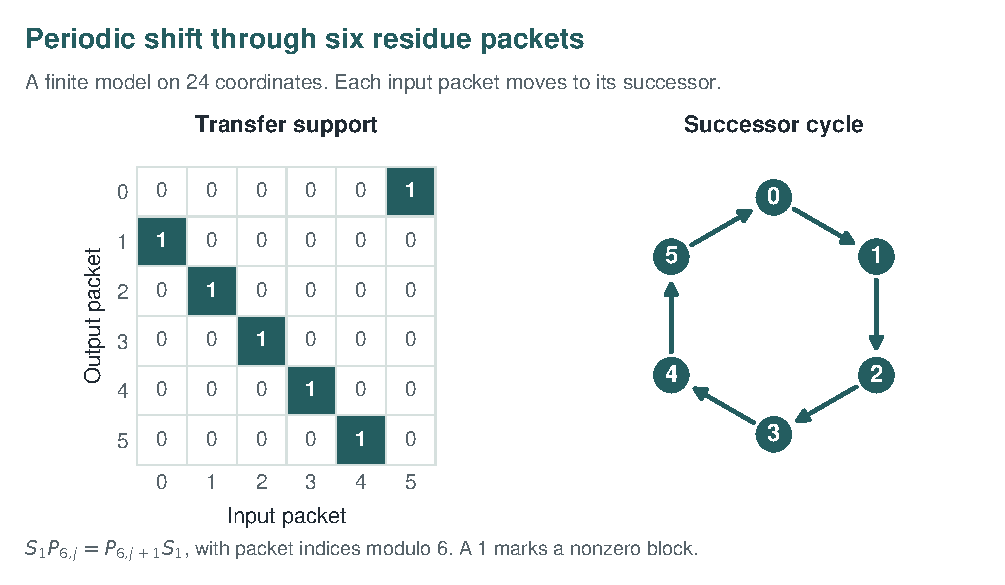
\includegraphics[width=0.96\textwidth]{07_shift_packet_transfer.pdf}
\caption{Support among residue packets in the periodic shift model on 24 coordinates with six packets. Each input residue transfers into the next output residue. The theorem for the infinite bilateral shift is established separately in the text.}
\label{fig:shift-transfer}
\end{figure}

\begin{boundary}
This section uses residue packets only to demonstrate the foundational transfer algebra. Nested refinement and structures for filter banks require additional definitions and are outside Chapter I.
\end{boundary}

\section{Worked matrix models}

\subsection{The full matrix algebra}

Let $X=\bbk^n$ and let $\cA=M_n(\bbk)=\End_{\bbk}(X)$, with the full matrix algebra declared before a seed or target is chosen. By \cref{cor:full-matrix}, every nonzero seed is cyclic. This is the maximal linear grammar on $X$. It does not give a compression result. Under a smaller declared operator algebra, the same vector need not be cyclic.

\subsection{Companion operators and repeated blocks}

For one operator $T$, \cref{thm:single-operator} turns verified primary data
into an exact certificate for the minimum number of seeds.  The numerical companion compares:
\begin{enumerate}[label=(\alph*)]
\item a nilpotent companion operator with one Jordan chain, for which the Krylov rank is $1,2,\ldots,n$.
\item two equal Jordan blocks, for which one diagonal seed produces a chain only as long as one block and then stalls.
\end{enumerate}

The observed stall is not numerical failure.  The associated
scalar quotient of dimension two certifies the lower bound in
\cref{thm:single-operator}. Identifying that quotient with the space that
measures geometric multiplicity is the classical Jordan input stated above.

\section{Worked graph model: adjacency algebras}

Let $G$ be a nonempty finite graph with adjacency matrix $A_G$, and regard
$\bbk^{V(G)}$ as a module over $\bbk[A_G]$.  The general result applies directly to a spectral certificate. For a symmetric real adjacency matrix, the classical spectral theorem supplies such data.

Within one eigenspace, every polynomial in the adjacency operator acts by a scalar. A seed therefore supplies at most one vector direction in that eigenspace. Distinct eigenvalues can be separated by projector polynomials, so the same seed may supply one direction to each of several eigenspaces. With a complete eigenbasis, the largest eigenspace determines how many seeds are needed, rather than the number of distinct eigenvalues.

\begin{corollary}[Certified graph seed number]
\label{cor:graph-rank}
Let $\bbk$ be a field and let $\Lambda$ be a nonempty finite set.  Suppose
there are pairwise distinct scalars $a_{\lambda}\in\bbk$, multiplicities
$m_{\lambda}\in\N$, and an eigenbasis
\[
\{b_{\lambda,j}:\lambda\in\Lambda,\ 1\le j\le m_{\lambda}\}
\]
of $\bbk^{V(G)}$ satisfying
\[
A_Gb_{\lambda,j}=a_{\lambda}b_{\lambda,j}.
\]
If $m_{\lambda}\le R$ for all $\lambda$ and
$m_{\lambda_*}=R$ for some $\lambda_*$, then $R$ is the least natural number
of adjacency seeds:
\[
{
R=\min\left\{r\in\N:
\begin{array}{l}
\text{there exist }s_1,\ldots,s_r\text{ with}\\[2pt]
\bbk^{V(G)}=\Span_{\bbk}
  \{p(A_G)s_j:p\in\bbk[t],\ 1\le j\le r\}
\end{array}
\right\}.
}
\]
\end{corollary}

\begin{proof}
The distinct eigenvalue labels give Lagrange polynomials that project onto
the individual eigenspace packets.  Padding one basis vector from every
packet into each of $R$ seeds gives the upper bound.  Projection to the
$m_{\lambda}$ eigenspace coordinates is a surjective scalar quotient, so any
generating family has at least $m_{\lambda}$ members for every $\lambda$.
The label $\lambda_*$ gives the matching lower bound $R$.
\end{proof}

\begin{boundary}[Input from spectral classification]
For a finite undirected graph over $\C$, the spectral theorem for real symmetric matrices
classically supplies a certificate of the displayed kind, and the numbers
$m_{\lambda}$ are the usual eigenvalue multiplicities. See
\cite{brouwerHaemers2012}.  The formal declaration verifies the
formula for the number of seeds from the supplied eigenbasis and distinct eigenvalue
labels.  It does not derive diagonalizability from symmetry or implement an
eigensolver.
\end{boundary}

\subsection{Path graphs}

For every field $\bbk$ and every $n\ge1$, an endpoint of $P_n$ is a cyclic
vector for the adjacency operator.  Consequently one is the least finite
number of adjacency seeds:
\[
{
1=\min\left\{r\in\N:
\exists s_1,\ldots,s_r,\quad
\bbk^n=\Span_{\bbk}\{p(A_{P_n})s_j:p\in\bbk[t],\ 1\le j\le r\}
\right\}.
}
\]
Over $\C$, the familiar spectral description has the distinct eigenvalues
\[
\lambda_k=2\cos\frac{k\pi}{n+1},
\qquad 1\le k\le n,
\]
and the normalized eigenvectors have endpoint coordinate proportional to
\[
\sin\frac{k\pi}{n+1}\ne0.
\]
There is also a combinatorial proof valid over every field.  Let
\[
K_n=[e_1,Ae_1,\ldots,A^{n-1}e_1].
\]
Its $(i,j)$ entry counts walks of length $j-1$ from the first vertex to vertex $i$. This entry is zero when $i>j$, while the diagonal entry is one because there is a unique shortest walk of length $i-1$ from vertex $1$ to vertex $i$. Hence $K_n$ is upper triangular with unit diagonal, so
\[
\det K_n=1
\qquad(n\ge1).
\]
Thus the endpoint is cyclic for every path size, not merely for the tested range.

\begin{figure}[htbp]
\centering
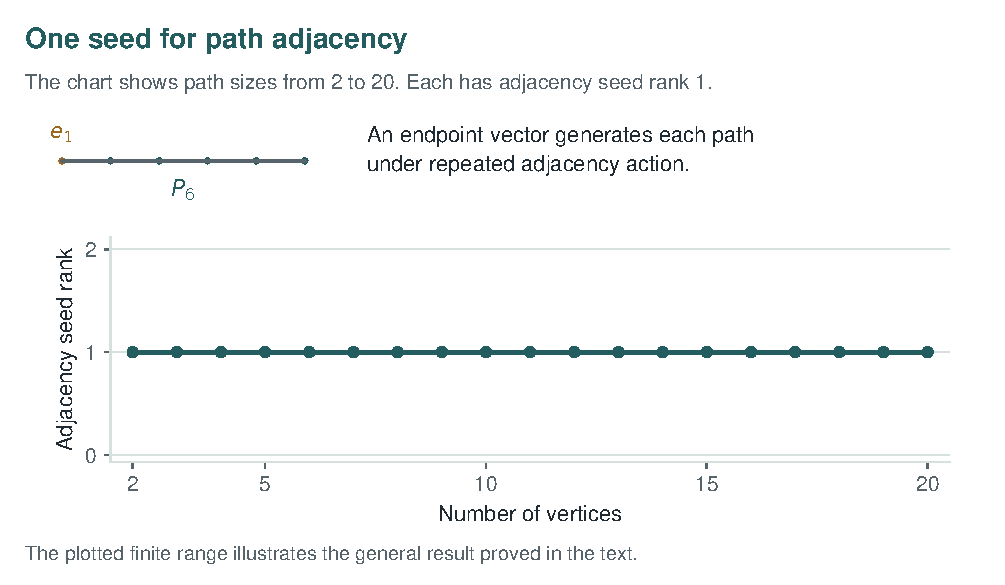
\includegraphics[width=0.96\textwidth]{05_path_graph_seed_rank.pdf}
\caption{The endpoint Krylov certificate gives every nonempty path one adjacency seed.}
\label{fig:path-rank}
\end{figure}

\subsection{Cycle graphs}

Two adjacent vertex vectors generate the adjacency module of every simple
cycle.  Over $\C$, a Fourier quotient built from a primitive root of unity supplies a matching
scalar obstruction of dimension two.  Hence, for every $n\ge3$, two is the
least finite number of adjacency seeds:
\[
{
2=\min\left\{r\in\N:
\exists s_1,\ldots,s_r,\quad
\C^n=\Span_{\C}\{p(A_{C_n})s_j:p\in\C[t],\ 1\le j\le r\}
\right\}.
}
\]
To see the upper bound directly, index the vertices modulo $n$.
The identity $Ae_j=e_{j-1}+e_{j+1}$ recovers successive vertex vectors
from $e_0$ and $e_1$, over any field. For the lower bound over $\C$, let
$\zeta$ be a primitive $n$th root of unity and define
\[
q(x)=\left(\sum_{j=0}^{n-1}\zeta^j x_j,
             \sum_{j=0}^{n-1}\zeta^{-j}x_j\right).
\]
Then $q(Ax)=(\zeta+\zeta^{-1})q(x)$. The images of $e_0$ and $e_1$
are $(1,1)$ and $(\zeta,\zeta^{-1})$, which are independent because
$\zeta\ne\zeta^{-1}$ for $n\ge3$. Thus $q$ is a scalar quotient
of dimension two, and \cref{prop:scalar-quotient} gives the
matching lower bound.

The usual spectral description writes the eigenvalues as
\[
\lambda_k=2\cos\frac{2\pi k}{n},
\qquad 0\le k<n.
\]
The values for $k$ and $n-k$ coincide. Apart from the simple characters at $k=0$ and, for even $n$, $k=n/2$, the remaining Fourier characters occur in pairs. Therefore the maximum eigenspace multiplicity is two, although some eigenspaces have multiplicity one, and
the certified minimum above is two.

\begin{figure}[htbp]
\centering
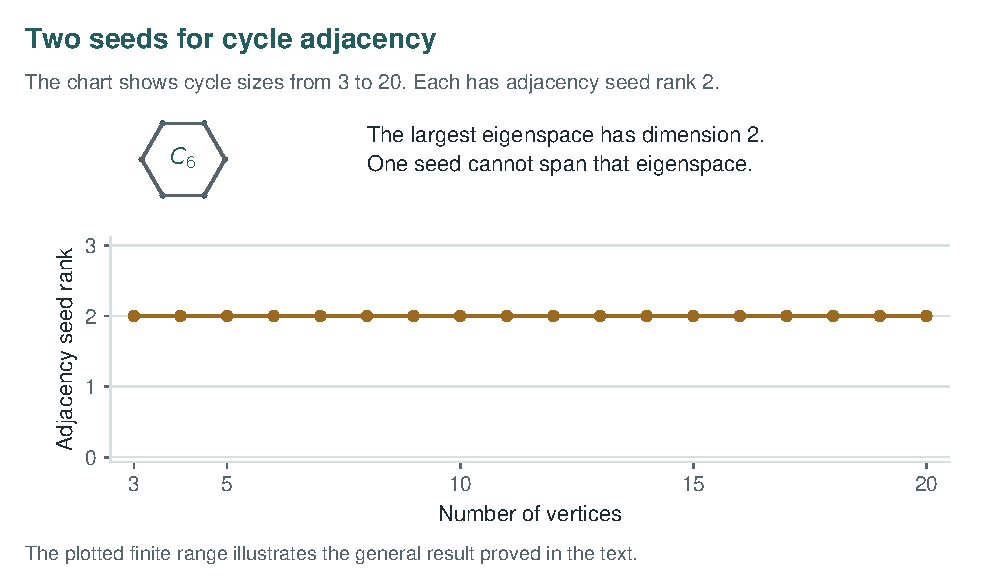
\includegraphics[width=0.96\textwidth]{06_cycle_graph_seed_rank.pdf}
\caption{Cycle graphs have maximum eigenspace multiplicity two for the adjacency operator and therefore require two adjacency seeds, although one or two exceptional eigenspaces are simple.}
\label{fig:cycle-rank}
\end{figure}

The path and cycle examples use nearly identical local operators.  Their
minimum finite seed numbers differ because the path has an
endpoint Krylov basis, whereas the cycle has a Fourier
quotient obstruction of dimension two.

\section{The common operator language}

The preceding examples can be written without changing the foundational notation.

\begin{longtable}{L{0.12\textwidth}L{0.13\textwidth}L{0.19\textwidth}L{0.17\textwidth}L{0.16\textwidth}}
\caption{Foundational realizations of the common operator language.}\label{tab:dictionary}\\
\toprule
Realization & Seed & Operator grammar & Packets & Completion or quotient \\
\midrule
\endfirsthead
\toprule
Realization & Seed & Operator grammar & Packets & Completion or quotient \\
\midrule
\endhead
Coordinate ring & $1$ & $M_x,M_y$ & even/odd $y$ degree & quotient by $y^2-x^3+x$ \\
Shift system & $\delta_0$ & $(S_m)_{m\in\Z}$ & residue classes of $n$ & $\ell^2$ closure \\
Full matrix module & $s\ne0$ & $M_n(\bbk)$ & chosen idempotents & finite dimensional \\
Single operator & $s_1,\ldots,s_r$ & $\bbk[T]$ & primary or spectral & finite dimensional \\
Graph adjacency & vertex seeds & $\bbk[A_G]$ & eigenspaces & finite dimensional \\
Typed grammar & vertex seeds & path algebra $\bbk Q/I$ & vertex idempotents & relation quotient \\
\bottomrule
\end{longtable}

\Needspace{16\baselineskip}
For a finite ordered seed family $S=(s_1,\ldots,s_r)$, let $\varepsilon_S:\cA^{\oplus r}\to X$ be the seed evaluation map of \cref{def:seed-evaluation}.  Its kernel is the relation module.  The free module modulo that kernel presents the generated hull by \cref{thm:free-presentation}.  The invariant content is:
\[
{
\begin{aligned}
&\text{generated hull: }\Hull_{\cA}(S),\\
&\text{seed complexity: }\srank_{\cA}(X),\\
&\text{packet coordinates: }x\leftrightarrow(P_{\alpha}x)_{\alpha},\\
&\text{operator coordinates: }T\leftrightarrow(P_{\beta}TP_{\alpha})_{\beta,\alpha},\\
&\text{relation module: }N_S:=\Ker\varepsilon_S\leq\cA^{\oplus r},\\
&\text{free presentation: }\cA^{\oplus r}/N_S\cong\Hull_{\cA}(S),\\
&\text{coordinate invariance: }P_{\alpha}\mapsto UP_{\alpha}U^{-1},\\
&\text{realization: }\Phi A=\varphi(A)\Phi.
\end{aligned}
}
\]

\begin{figure}[htbp]
\centering
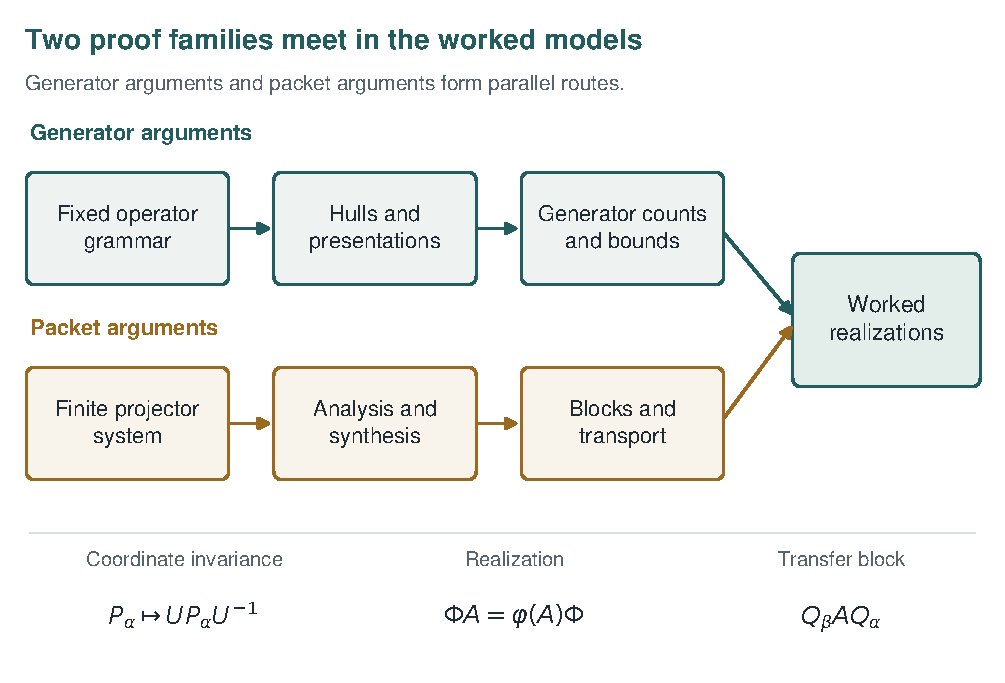
\includegraphics[width=0.96\textwidth]{10_theorem_dependency.pdf}
\caption{Structural overview of the two proof families. The generator and packet arguments meet in the worked realizations. This diagram is not an exhaustive graph of Lean declaration dependencies.}
\label{fig:dependency}
\end{figure}

\section{Computational certificates}

The accompanying Python package is not used as a substitute for proof. It provides exact symbolic checks and finite numerical regression tests for formulas already proved. The computed ranges and random seeds are recorded explicitly. These checks do not extend a theorem beyond its hypotheses or certify an unrestricted numerical implementation. The journal companion also tests integer counts beyond the precision of floating point arithmetic and rejects the unsupported spectral shortcut for complex symmetric matrices.

\subsection{Test suite}

The test suite checks:
\begin{enumerate}[label=(\roman*)]
\item projector idempotence, annihilation, and completeness.
\item exact vector analysis and synthesis.
\item exact operator reconstruction from all transfer blocks.
\item coordinate transport under a dense random similarity transform.
\item cyclicity of a companion operator.
\item the obstruction that requires two seeds for repeated Jordan blocks.
\item the semisimple multiplicity formula in representative cases.
\item full orbit dimension for two representative nonzero seeds under the full matrix algebra.
\item exact reduction and packet multiplication in the elliptic coordinate ring.
\item seed ranks of path and cycle adjacency modules over the reported finite ranges.
\item the cyclic residue transfer pattern of a finite shift.
\end{enumerate}

\subsection{Recorded results}

\begin{table}[htbp]
\centering
\caption{Representative finite checks recorded for the worked models. The computational companion distinguishes these records from its separately verified runs.}
\label{tab:results}
\begin{tabular}{L{0.57\textwidth}r}
\toprule
Quantity & Result \\
\midrule
Projector idempotence residual & $0$ \\
Projector annihilation residual & $0$ \\
Projector completeness residual & $0$ \\
Operator reconstruction residual & $0$ \\
Residual for transported projectors, maximum & $1.85\times10^{-15}$ \\
Companion seed rank & $1$ \\
Two equal Jordan blocks, seed rank & $2$ \\
$M_3(\C)$ acting on seven copies, seed rank & $3$ \\
Sampled path graph seed ranks, $2\le n\le12$ & $1$ \\
Sampled cycle graph seed ranks, $3\le n\le12$ & $2$ \\
Full $M_4(\R)$ orbit dimensions for two sampled nonzero seeds & $4,4$ \\
Automated tests & $33/33$ passed \\
\bottomrule
\end{tabular}
\end{table}

The finite shift pattern recovered by the experiment is
\[
\begin{pmatrix}
0&0&0&1\\
1&0&0&0\\
0&1&0&0\\
0&0&1&0
\end{pmatrix},
\]
which is the exact packet adjacency of a cyclic transfer among four phases.

\subsection{Algorithms}

The following finite constructions state mathematical specifications for the companion. Their Lean counterparts and exact scope are listed in the separate guide. They do not assert code extraction or a particular backend's performance.

\begin{construction}[Closure specification for the orbit hull]
\label{con:orbit-hull-algorithm}
Let $V$ have finite dimension, let $(O_i)_{i\in I}$ be a finite operator
family, and let $S\subseteq V$.  Define
\[
W_0=\Span_{\bbk}S,
\qquad
W_{n+1}=W_n+\sum_{i\in I}O_i(W_n).
\]
Then there is an $n\in\N$ such that
\[
W_{n+1}=W_n
\qquad\text{and}\qquad
W_n=\Hull_{(O_i)}(S),
\]
where the right side is the least subspace containing $S$ and invariant under
every $O_i$.  Thus the ascending subspace iteration terminates and its stable
value is exactly the finite operator hull.

Each strict enlargement increases dimension, so finite dimension prevents the iteration from continuing indefinitely. Equality at one step means that applying any declared operator keeps every vector in the current subspace. The stable subspace is therefore invariant, while every earlier step belongs to any invariant subspace that contains the seeds.
\end{construction}

\begin{construction}[Table specification for transfer blocks]
\label{con:transfer-block-algorithm}
Given finite projector systems $(P_i)_{i\in I}$ and $(Q_j)_{j\in J}$ and a
linear map $T$, form the table
\[
B_{ji}=Q_jTP_i.
\]
Its assembly reconstructs the input map exactly,
\[
\sum_{j\in J}\sum_{i\in I}B_{ji}=T,
\]
and its reported support relation is exactly
$\{(i,j):B_{ji}\ne0\}$.  The latter equality is the specification of the
transfer graph output. It does not claim that Lean extracts a routine that decides the edge list for every coefficient field.
\end{construction}

\begin{construction}[Exact graph seed rank from a certificate]
\label{con:exact-graph-seed-rank}
For a finite square matrix $A$ over a field $K$, define the noncomputable exact
spectral quantity
\[
r_{\mathrm{spec}}(A)
=
\max_{\mu\in\Spec_K(A)}
\dim_K\ker(A-\mu I),
\]
with value zero for an empty spectrum.  Suppose an exact certificate supplies
a finite eigenbasis indexed by labels and multiplicities, the eigenvalue
equations, a multiplicity bound attained by one label, projector polynomials
that extract the padded eigenbasis generators, coverage of every spectral
value by a label, equality of the declared and actual eigenspace dimensions,
and membership of the maximizing eigenvalue in the spectrum.  Then
$r_{\mathrm{spec}}(A)$ is the least natural number of seeds under polynomial orbits
for $A$.

This is a verified certificate checker/specification.  It does not construct
the eigenbasis, prove that a symmetric matrix is diagonalizable, or implement
an exact eigensolver.  The companion Python code performs symbolic
computations in the reported finite graph range. The path and cycle
results for every size are proved separately above.
\end{construction}


\section{Reading guide: common confusions and diagnostic questions}

\subsection{Common confusions}
\begin{center}
\begin{longtable}{@{}>{\raggedright\arraybackslash}p{0.26\textwidth}>{\raggedright\arraybackslash}p{0.68\textwidth}@{}}
\toprule
\textbf{Do not conflate} & \textbf{Correct distinction}\\
\midrule
\endhead
Grammar with realized algebra & The grammar may contain relations or words that act as zero.  Seed rank depends only on the image action.\\
Seed with basis vector & A seed is a generator under an algebra action.  One seed may generate a module with large dimension.\\
Cyclic vector with eigenvector & A cyclic vector must generate the whole module under operator words.  It is usually not an eigenvector.\\
Packet with orthogonal subspace & A packet is the range of an idempotent in a complete annihilating family.  Orthogonality is optional.\\
Exact reconstruction with good conditioning & Algebraic inverse identities may coexist with large analysis and synthesis norms.\\
Nonzero transfer edge with surjective transfer & A nonzero block can have small rank.  Graph reachability alone does not prove generation.\\
Seed rank for single packet seeds with unrestricted seed rank & Seeds supported in several packets may meet several source components simultaneously.\\
Continuous surjection with quotient isomorphism & The target topology must agree with the quotient topology.\\
Repeated notation with semantic realization & A true realization must preserve a declared collection of operations and identities.\\
\bottomrule
\end{longtable}
\end{center}

\subsection{Diagnostic questions for a new application}
Before claiming that a new subject is a realization of Chapter I, answer the following.
\begin{enumerate}
\item What is the fixed operator grammar or acting algebra?
\item What is the concrete realization space or module?
\item Which seeds are declared before the target is chosen?
\item Is generation algebraic, topological, probabilistic, or approximate?
\item What are the idempotent packets, and in what sense do they sum to the identity?
\item Are the packets finite, countable unconditional, or merely formal?
\item What are the transfer blocks, and which blocks are known to vanish?
\item Which morphisms preserve the packet system?
\item Which quotient, completion, tensor, or limit operations must be preserved?
\item What exact theorem from Chapter I is being specialized, and what new domain theorem remains to be proved?
\end{enumerate}

\subsection{Theorem spine at a glance}
\ConceptChain{
\(
\begin{array}{c}
\text{free seed presentation}\\[0.25em]
\Downarrow\\[-0.1em]
\text{minimal generator number}\\[0.25em]
\Downarrow\\[-0.1em]
\text{reduction modulo the Jacobson radical}\\[0.25em]
\Downarrow\\[-0.1em]
\text{semisimple or primary computation}
\end{array}
\qquad\qquad
\begin{array}{c}
\text{packet idempotents}\\[0.25em]
\Downarrow\\[-0.1em]
\text{exact analysis/synthesis}\\[0.25em]
\Downarrow\\[-0.1em]
\text{transfer block algebra}\\[0.25em]
\Downarrow\\[-0.1em]
\text{graphs, quotients, and realization}
\end{array}
\)
}


\section{Notation and convention ledger}
\begin{multicols}{2}
\begin{description}[style=nextline,font=\normalfont\bfseries]
\item[Address.] An operator word applied to a seed.
\item[Analysis.] The map sending an object to all packet coordinates.
\item[Block support.] The set of packet pairs \((\beta,\alpha)\) for which \(P_\beta TP_\alpha\neq0\).
\item[Collapsed realization.] The direct sum of all typed vertex spaces.
\item[Condensation graph.] The acyclic graph obtained by collapsing strongly connected components.
\item[Generated hull.] The submodule generated by a seed family, or its declared closure.
\item[Grammar.] A typed quiver and relation ideal describing legal operator words.
\item[Packet.] The range of one idempotent in a complete annihilating family.
\item[Packet pure.] Supported in at most one packet.
\item[Preservation profile.] The operations a realization functor is required to preserve.
\item[Realized algebra.] The image of the grammar algebra in the endomorphism algebra of a realization.
\item[Seed rank.] The smallest cardinality of a generating family. For a finite value, this is the minimum number of seeds.
\item[Source component.] A strongly connected component with no incoming edge in the condensation graph.
\item[Synthesis.] The map adding packet coordinates into the original object.
\item[Transfer block.] The map from one packet space to another obtained by sandwiching an operator between packet projectors.
\item[Transfer graph.] The directed graph formed from nonzero blocks of a declared algebra generating family.
\end{description}
\end{multicols}

\begin{sectionrecap}[title={How to use the chapter after the first reading}]
For a concrete calculation, first reduce the action to the realized algebra.  Next compute or bound seed rank using quotients, the module top, or primary decomposition.  Then declare the packet system and use exact analysis and synthesis.  Finally move all operator equations into transfer blocks, where support, graph, quotient, and functorial constraints become explicit.
\end{sectionrecap}


\section{Proof dependency spine}

\small
\begin{longtable}{@{}p{0.42\textwidth}p{0.52\textwidth}@{}}
\toprule
\textbf{Canonical record} & \textbf{Immediate proof dependencies}\\
\midrule
\endfirsthead
\toprule
\textbf{Canonical record} & \textbf{Immediate proof dependencies}\\
\midrule
\endhead
\texttt{PSC-I-T-TYPED-MODULE-EQUIVALENCE} & Typed grammar and path algebra action.\\
\texttt{PSC-I-T-FREE-PRESENTATION} & Seed evaluation map and first isomorphism theorem.\\
\texttt{PSC-I-T-COMPLETED-PRESENTATION} & Free presentation and uniqueness of completion.\\
\texttt{PSC-I-T-QUOTIENT-MONOTONICITY} & Intertwining identity and generated hull.\\
\texttt{PSC-I-T-EXACT-SEQUENCE-BOUNDS} & Quotient monotonicity and lifting generators.\\
\texttt{PSC-I-T-MODULE-TOP} & Nakayama lemma.\\
\texttt{PSC-I-T-SEMISIMPLE-SEED-RANK} & Module top theorem and regular module multiplicities.\\
\texttt{PSC-I-T-SINGLE-OPERATOR} & Primary decomposition, local formula, and product action.\\
\texttt{PSC-I-T-EXACT-PACKET-COORDINATES} & Complete finite idempotent family.\\
\texttt{PSC-I-T-COUNTABLE-}\newline\texttt{UNCONDITIONAL-PACKETS} & Completeness of the unconditional coordinate space.\\
\texttt{PSC-I-T-BLOCK-ALGEBRA} & Reconstruction and block multiplication.\\
\texttt{PSC-I-T-SUPPORT-PATTERN-ALGEBRA} & Block multiplication and rank one necessity tests.\\
\texttt{PSC-I-T-PREORDER-}\newline\texttt{ALGEBRA-DECOMPOSITION} & Preorder support criterion and finite chain nilpotence.\\
\texttt{PSC-I-T-ALGEBRA-}\newline\texttt{REACHABILITY-SUPPORT} & Generator word packet expansion.\\
\texttt{PSC-I-T-SOURCE-COMPONENT-SEED-RANK} & Reachability obstruction and edge surjective propagation.\\
\texttt{PSC-I-T-NATURALITY} & Intertwining and packet aggregation.\\
\texttt{PSC-I-T-PACKET-EXACT-SEQUENCE} & Invariant packet projectors and first isomorphism theorem.\\
\texttt{PSC-I-T-DENSE-REALIZATION} & Continuity and naturality of hulls.\\
\texttt{PSC-I-T-REALIZATION-EXPORT} & Additive functor axioms and preserved universal constructions.\\
\bottomrule
\end{longtable}
\normalsize

\clearpage\section{Conclusions and further use}

The results establish the following tools for working with a declared operator action and packet system:
\begin{enumerate}[label=\textbf{I.\arabic*.},leftmargin=*,itemsep=0.3em,topsep=0.4em]
\item The two sided annihilator criterion is proved in \cref{prop:two-sided-annihilator}.
\item Generator detection modulo the Jacobson radical is proved in \cref{thm:module-top}.
\item The semisimple seed rank formula applies over arbitrary division rings, with the conventions for left and right modules kept explicit in \cref{thm:semisimple-seed-rank}.
\item The single operator formula and its cyclic criteria apply over arbitrary fields in \cref{thm:single-operator,cor:cyclic-matrix}.
\item The countable unconditional packet theorem is proved in \cref{thm:countable-packets}.
\item The classification of support compatible with $*$ is proved in \cref{cor:star-support}.
\item The weighted source component formula gives the packet pure generation requirement under the propagation hypotheses in \cref{thm:source-component-rank}.
\item Seed system composition, packet exact sequences, quotient block descent, dense realization, quotient completion, and semantic theorem transport are proved in \cref{prop:seed-category,thm:packet-exact-sequence,cor:block-descent,thm:dense-realization,thm:quotient-topology,thm:realization-export}.
\item Exact sequence bounds, monotonicity under enlargement of the acting algebra, coordinate stability, projection onto diagonal blocks, and preorder decomposition are established in \cref{thm:exact-sequence-bounds,prop:acting-algebra-monotonicity,prop:conditioned-coordinates,prop:block-diagonal-projection,thm:preorder-decomposition}.
\end{enumerate}

\clearpage\appendix
\section{Stable statement concordance}\label{app:stable-concordance}
These identifiers preserve the expanded foundation's namespace of 108 records. The display numbers refer to Chapter I. The identifiers track mathematical statements, and their count does not measure how many theorems have been verified in Lean. Statements in the worked models retain their source labels and are mapped separately by the Lean guide.
\small\begin{longtable}{@{}p{.44\textwidth}p{.07\textwidth}p{.41\textwidth}@{}}
\toprule Stable identifier & No. & Statement\\\midrule\endhead
\nolinkurl{PSC-I-D-COEFFICIENT-REGIME} & \ref{def:coefficient-regime} & Coefficient and module regimes \\
\nolinkurl{PSC-I-D-THEOREM-RECORD} & \ref{def:theorem-record} & Canonical theorem record \\
\nolinkurl{PSC-I-B-SYMBOLIC-SCOPE} & \ref{bnd:symbolic-scope} & Symbolic scope \\
\nolinkurl{PSC-I-D-TYPED-GRAMMAR} & \ref{def:typed-grammar} & Typed operator grammar \\
\nolinkurl{PSC-I-D-COLLAPSED-REALIZATION} & \ref{def:collapsed-realization} & Collapsed one space realization \\
\nolinkurl{PSC-I-T-TYPED-MODULE-EQUIVALENCE} & \ref{thm:typed-module-equivalence} & Typed realization and module equivalence \\
\nolinkurl{PSC-I-D-REALIZED-ALGEBRA} & \ref{def:realized-algebra} & Realized operator algebra \\
\nolinkurl{PSC-I-P-ACTION-FACTORIZATION} & \ref{prop:action-factorization} & Action factorization and hull invariance \\
\nolinkurl{PSC-I-D-SEED-SYSTEM} & \ref{def:seed-system} & Linear seed system \\
\nolinkurl{PSC-I-D-GENERATED-HULL} & \ref{def:generated-hull} & Generated hull \\
\nolinkurl{PSC-I-D-NATURAL-PRESENTATION} & \ref{def:natural-presentation} & Natural presentation \\
\nolinkurl{PSC-I-P-ALGEBRA-MODULE-GENERATION} & \ref{prop:algebra-module-generation} & Algebra generation and module generation are distinct \\
\nolinkurl{PSC-I-B-TARGET-DEPENDENT-OPERATORS} & \ref{bnd:target-dependent-operators} & Target dependent operators \\
\nolinkurl{PSC-I-D-SEED-EVALUATION} & \ref{def:seed-evaluation} & Seed evaluation map \\
\nolinkurl{PSC-I-T-FREE-PRESENTATION} & \ref{thm:free-presentation} & Finite free presentation \\
\nolinkurl{PSC-I-C-MINIMAL-FREE-COVER} & \ref{cor:minimal-free-cover} & Minimal free cover characterization \\
\nolinkurl{PSC-I-C-ONE-SEED-PRESENTATION} & \ref{cor:one-seed-presentation} & One seed presentation \\
\nolinkurl{PSC-I-P-ANNIHILATOR-TWO-SIDED} & \ref{prop:two-sided-annihilator} & Two sided annihilator criterion \\
\nolinkurl{PSC-I-T-COMPLETED-PRESENTATION} & \ref{thm:completed-presentation} & Completion of a dense free presentation \\
\nolinkurl{PSC-I-D-SEED-RANK} & \ref{def:seed-rank} & Seed rank \\
\nolinkurl{PSC-I-P-CYCLIC-CHARACTERIZATION} & \ref{prop:cyclic-characterization} & Cyclic characterization \\
\nolinkurl{PSC-I-P-ACTING-ALGEBRA-MONOTONICITY} & \ref{prop:acting-algebra-monotonicity} & Monotonicity under enlargement of the acting algebra \\
\nolinkurl{PSC-I-T-QUOTIENT-MONOTONICITY} & \ref{thm:quotient-monotonicity} & Quotient monotonicity \\
\nolinkurl{PSC-I-C-ISOMORPHISM-INVARIANCE} & \ref{cor:isomorphism-invariance} & Isomorphism invariance \\
\nolinkurl{PSC-I-T-EXACT-SEQUENCE-BOUNDS} & \ref{thm:exact-sequence-bounds} & Short exact sequence bounds \\
\nolinkurl{PSC-I-P-SHARED-DIRECT-SUM} & \ref{prop:shared-direct-sum} & Shared direct sum bounds \\
\nolinkurl{PSC-I-T-INDEPENDENT-DIRECT-SUM} & \ref{thm:independent-direct-sum} & Independent direct sum formula \\
\nolinkurl{PSC-I-P-TENSOR-BOUND} & \ref{prop:tensor-bound} & Tensor product bound \\
\nolinkurl{PSC-I-B-TENSOR-NONEQUALITY} & \ref{bnd:tensor-nonequality} & Tensor rank is not generally multiplicative \\
\nolinkurl{PSC-I-P-SCALAR-EXTENSION-MONOTONICITY} & \ref{prop:scalar-extension} & Scalar extension monotonicity \\
\nolinkurl{PSC-I-D-SEED-RANK-WITNESS} & \ref{def:seed-rank-witness} & Seed rank witness \\
\nolinkurl{PSC-I-P-SCALAR-QUOTIENT-WITNESS} & \ref{prop:scalar-quotient} & Scalar quotient witness \\
\nolinkurl{PSC-I-CI-NAKAYAMA} & \ref{ci:nakayama} & Nakayama lemma \\
\nolinkurl{PSC-I-T-MODULE-TOP} & \ref{thm:module-top} & Generator number is detected modulo the Jacobson radical \\
\nolinkurl{PSC-I-C-LOCAL-ALGEBRA-FORMULA} & \ref{cor:local-algebra-formula} & Local algebra formula \\
\nolinkurl{PSC-I-CI-WEDDERBURN-ARTIN} & \ref{ci:wedderburn} & Wedderburn and Artin decomposition \\
\nolinkurl{PSC-I-L-REGULAR-MODULE-MULTIPLICITIES} & \ref{lem:regular-multiplicities} & Regular module multiplicities \\
\nolinkurl{PSC-I-T-SEMISIMPLE-SEED-RANK} & \ref{thm:semisimple-seed-rank} & Semisimple seed rank formula over arbitrary division rings \\
\nolinkurl{PSC-I-C-ALGEBRAICALLY-CLOSED-FORMULA} & \ref{cor:algebraically-closed-formula} & Algebraically closed multiplicity formula \\
\nolinkurl{PSC-I-C-FULL-MATRIX} & \ref{cor:full-matrix} & Full matrix algebra \\
\nolinkurl{PSC-I-C-MULTIPLICITY-OBSTRUCTION} & \ref{cor:multiplicity-obstruction} & Multiplicity obstruction \\
\nolinkurl{PSC-I-CI-PID-PRIMARY-DECOMPOSITION} & \ref{ci:primary-decomposition} & Primary decomposition for polynomial modules \\
\nolinkurl{PSC-I-T-SINGLE-OPERATOR} & \ref{thm:single-operator} & Single operator seed rank \\
\nolinkurl{PSC-I-C-INVARIANT-FACTOR-COUNT} & \ref{cor:invariant-factor-count} & Invariant factor count \\
\nolinkurl{PSC-I-C-ALGEBRAICALLY-CLOSED-SINGLE-OPERATOR} & \ref{cor:geometric-multiplicity} & Geometric multiplicity formula \\
\nolinkurl{PSC-I-C-CYCLIC-MATRIX} & \ref{cor:cyclic-matrix} & Cyclic matrix criterion \\
\nolinkurl{PSC-I-D-PACKET-SYSTEM} & \ref{def:packet-system} & Finite packet system \\
\nolinkurl{PSC-I-D-PACKET-SUPPORT} & \ref{def:packet-support} & Packet support and packet pure vectors \\
\nolinkurl{PSC-I-L-PACKET-AGGREGATION} & \ref{lem:packet-aggregation} & Finite packet aggregation \\
\nolinkurl{PSC-I-D-ANALYSIS-SYNTHESIS} & \ref{def:analysis-synthesis} & Packet analysis and synthesis \\
\nolinkurl{PSC-I-T-EXACT-PACKET-COORDINATES} & \ref{thm:exact-packet-coordinates} & Exact packet coordinate isomorphism \\
\nolinkurl{PSC-I-C-PACKETWISE-EQUALITY} & \ref{cor:packetwise-equality} & Packetwise equality \\
\nolinkurl{PSC-I-C-PACKET-UNIVERSAL-PROPERTY} & \ref{cor:packet-universal-property} & Universal mapping property of finite packet coordinates \\
\nolinkurl{PSC-I-T-TENSOR-PACKET-SYSTEM} & \ref{thm:tensor-packet-system} & Tensor product packet systems \\
\nolinkurl{PSC-I-P-DUAL-PACKET-SYSTEM} & \ref{prop:dual-packet-system} & Dual packet systems \\
\nolinkurl{PSC-I-T-BANACH-PACKET-ISOMORPHISM} & \ref{thm:banach-packets} & Finite Banach packet isomorphism \\
\nolinkurl{PSC-I-D-PACKET-CONDITION-NUMBER} & \ref{def:packet-condition-number} & Packet coordinate condition number \\
\nolinkurl{PSC-I-P-CONDITIONED-COORDINATES} & \ref{prop:conditioned-coordinates} & Conditioned coordinate transport \\
\nolinkurl{PSC-I-C-COMPLETION-PACKET-SPLIT} & \ref{cor:completion-packet-split} & Completion preserves a finite packet split \\
\nolinkurl{PSC-I-D-UNCONDITIONAL-PACKET-SPACE} & \ref{def:unconditional-packet-space} & Unconditional packet sum space \\
\nolinkurl{PSC-I-L-UNCONDITIONAL-COMPLETENESS} & \ref{lem:unconditional-completeness} & Completeness of the unconditional packet sum \\
\nolinkurl{PSC-I-T-COUNTABLE-UNCONDITIONAL-PACKETS} & \ref{thm:countable-packets} & Countable unconditional packet isomorphism \\
\nolinkurl{PSC-I-R-UNIFORM-BOUNDEDNESS} & \ref{rem:uniform-boundedness} & Uniform boundedness \\
\nolinkurl{PSC-I-B-INFINITE-PACKET-TOPOLOGY} & \ref{bnd:infinite-packet-topology} & Infinite packet sums \\
\nolinkurl{PSC-I-D-TRANSFER-BLOCK} & \ref{def:transfer-block} & Transfer block \\
\nolinkurl{PSC-I-T-OPERATOR-RECONSTRUCTION} & \ref{thm:operator-reconstruction} & Exact operator reconstruction \\
\nolinkurl{PSC-I-T-BLOCK-MULTIPLICATION} & \ref{thm:block-multiplication} & Packet matrix multiplication \\
\nolinkurl{PSC-I-C-BLOCK-POWERS} & \ref{cor:block-powers} & Packet powers and paths \\
\nolinkurl{PSC-I-C-ADJOINT-REVERSAL} & \ref{cor:adjoint-reversal} & Adjoint reversal \\
\nolinkurl{PSC-I-C-TENSOR-TRANSFER-BLOCKS} & \ref{cor:tensor-transfer-blocks} & Tensor product transfer blocks \\
\nolinkurl{PSC-I-T-BLOCK-INTERTWINING} & \ref{thm:block-intertwining} & Blockwise intertwining equations \\
\nolinkurl{PSC-I-T-BLOCK-ALGEBRA} & \ref{thm:block-algebra} & Full block algebra representation \\
\nolinkurl{PSC-I-C-PACKET-SUPPORT-PROPAGATION} & \ref{cor:packet-support-propagation} & Propagation of packet support \\
\nolinkurl{PSC-I-C-DIMENSION-COUNT} & \ref{cor:dimension-count} & Dimension count \\
\nolinkurl{PSC-I-P-BLOCK-DIAGONAL-COMMUTANT} & \ref{prop:block-diagonal-projection} & Block diagonal projection and packet commutant \\
\nolinkurl{PSC-I-D-SUPPORT-RELATION} & \ref{def:support-relation} & Support relation and support space \\
\nolinkurl{PSC-I-T-SUPPORT-PATTERN-ALGEBRA} & \ref{thm:support-pattern} & Support pattern algebra criterion \\
\nolinkurl{PSC-I-C-SUPPORT-PATTERN-STAR} & \ref{cor:star-support} & Bounded support patterns closed under $*$ \\
\nolinkurl{PSC-I-T-PREORDER-ALGEBRA-DECOMPOSITION} & \ref{thm:preorder-decomposition} & Preorder support algebra decomposition \\
\nolinkurl{PSC-I-D-TRANSFER-GRAPH} & \ref{def:transfer-graph} & Transfer graph of an algebra generating family \\
\nolinkurl{PSC-I-T-ALGEBRA-REACHABILITY-SUPPORT} & \ref{thm:algebra-reachability-support} & Reachability support of the generated algebra \\
\nolinkurl{PSC-I-P-REACHABILITY-OBSTRUCTION} & \ref{prop:reachability-obstruction} & Reachability obstruction for generated hulls \\
\nolinkurl{PSC-I-D-DIRECTED-SEED-RANK} & \ref{def:directed-seed-rank} & Packet pure seed rank \\
\nolinkurl{PSC-I-P-PACKET-PURE-RANK-BOUNDS} & \ref{prop:packet-pure-rank-bounds} & Basic packet pure rank bounds \\
\nolinkurl{PSC-I-D-EDGE-SURJECTIVE} & \ref{def:edge-surjective} & Edge surjective packet system \\
\nolinkurl{PSC-I-T-SOURCE-COMPONENT-SEED-RANK} & \ref{thm:source-component-rank} & Source component formula for packet pure seed rank \\
\nolinkurl{PSC-I-D-PACKET-PROPAGATING} & \ref{def:packet-propagating} & Packet propagating system \\
\nolinkurl{PSC-I-C-SOURCE-COMPONENT-COUNT} & \ref{cor:source-component-count} & Unweighted source component count \\
\nolinkurl{PSC-I-B-PACKET-PURE-BOUNDARY} & \ref{bnd:packet-pure-boundary} & Mixed support seeds can merge source requirements \\
\nolinkurl{PSC-I-T-COORDINATE-TRANSPORT} & \ref{thm:coordinate-transport} & Coordinate transport \\
\nolinkurl{PSC-I-D-PACKET-MORPHISM} & \ref{def:packet-morphism} & Packet compatible operator morphism \\
\nolinkurl{PSC-I-D-SEED-MORPHISM} & \ref{def:seed-morphism} & Morphism of seeded systems \\
\nolinkurl{PSC-I-T-NATURALITY} & \ref{thm:naturality} & Naturality of generated hulls and transfer blocks \\
\nolinkurl{PSC-I-P-SEED-SYSTEM-CATEGORY} & \ref{prop:seed-category} & Category of seeded packet systems \\
\nolinkurl{PSC-I-T-PACKET-EXACT-SEQUENCE} & \ref{thm:packet-exact-sequence} & Packet exact sequence for an invariant subspace \\
\nolinkurl{PSC-I-T-QUOTIENT-PACKET-DESCENT} & \ref{thm:quotient-packet-descent} & Packet descent through an invariant quotient \\
\nolinkurl{PSC-I-C-QUOTIENT-PACKET-DESCENT} & \ref{cor:block-descent} & Restriction and quotient of transfer blocks \\
\nolinkurl{PSC-I-C-TOPOLOGICAL-PACKET-EXACT-SEQUENCE} & \ref{cor:topological-packet-exact-sequence} & Topological packet exact sequence \\
\nolinkurl{PSC-I-T-DENSE-REALIZATION} & \ref{thm:dense-realization} & Dense realization theorem \\
\nolinkurl{PSC-I-T-QUOTIENT-TOPOLOGY-COMPLETION} & \ref{thm:quotient-topology} & Quotient topology and completed realization \\
\nolinkurl{PSC-I-B-TOPOLOGICAL-QUOTIENT} & \ref{bnd:topological-quotient} & Continuous surjections and quotient topology \\
\nolinkurl{PSC-I-D-REALIZATION-FUNCTOR} & \ref{def:realization-functor} & Realization functor and preservation profile \\
\nolinkurl{PSC-I-T-REALIZATION-EXPORT} & \ref{thm:realization-export} & Equational realization principle \\
\nolinkurl{PSC-I-P-REALIZATION-EXPORT} & \ref{prop:realization-export} & Realization export principle \\
\nolinkurl{PSC-I-D-SEMANTIC-REALIZATION} & \ref{def:semantic-realization} & Semantic realization criterion \\
\nolinkurl{PSC-I-ALG-EXAMPLE-SLOTS} & \ref{def:reserved-example-slots} & Worked realization interface \\
\nolinkurl{PSC-I-EXPORT} & \ref{def:paper-one-export} & Chapter I export object \\
\nolinkurl{PSC-I-B-FINAL-CLAIM-BOUNDARY} & \ref{bnd:final-claim-boundary} & Exact limits of Chapter I \\
\bottomrule\end{longtable}\normalsize
\clearpage\section{Visual atlas}\label{app:visual-atlas}
The following twenty-two plates present exact finite models, explanatory diagrams, and one analytic density example. Each plate follows a calculation, identity, or obstruction from the main text. All graphics are generated from mathematical source, and the cross-references refer to the mathematical text.

\medskip
\begin{longtable}{@{}p{.08\textwidth}p{.82\textwidth}@{}}
\toprule Plate & Route through the examples\\\midrule\endhead
1, 2 & Fixed grammars, seed power, and the objects of the calculus.\\
3, 4 & Two linked chains and a quotient proving the minimum seed count.\\
5, 6 & Left ideal relations and typed reachability with a missing direction.\\
7, 8 & Oblique exact coordinates and complete transfer block multiplication.\\
9, 10 & Cancellation along paths and the algebra of admissible zero patterns.\\
11, 12 & Coordinate transport, shared action, and independent control.\\
13, 14 & Semisimple multiplicity budgets and primary extraction polynomials.\\
15, 16 & Path endpoints and the cycle's two dimensional quotient obstruction.\\
17 & A coordinate ring relation as a two packet product rule.\\
18, 19 & Dense shift generation, residue coordinates, and address carry.\\
20, 21 & Exact orbit hull stabilization and all tensor cross terms.\\
22 & The scope of mathematical, formal, and computational evidence.\\
\bottomrule\end{longtable}

The seed examples can be read consecutively. The packet and graph plates also provide entry points for readers interested in coordinates or propagation. The displayed matrices are exact. Numerical illustrations in the earlier figures retain their explicitly stated finite ranges. Each diagram is accompanied by the equation or obstruction it represents, so it can be read alongside the relevant proof.
\begingroup\fontsize{9.9}{11.2}\selectfont\setstretch{1.0}\setlength{\parindent}{0pt}\setlength{\parskip}{2pt}\setlength{\abovedisplayskip}{7pt}\setlength{\belowdisplayskip}{7pt}% A visual appendix of worked examples to the preserved Chapter I v1.2.1 manuscript.
% Every page starts explicitly, making overflow detectable by the build audit.

\vpage{1}{What can one seed actually do?}{CHAPTER I / A VISUAL APPENDIX OF WORKED EXAMPLES}{Main text: \cref{def:seed-rank,prop:acting-algebra-monotonicity,thm:exact-packet-coordinates}}
A seed does not carry a fixed amount of generative power by itself. The answer depends on the operators that are allowed to act on it. Chapter I makes that dependence part of the mathematical object rather than leaving it implicit.

Use the same space of dimension six throughout the first comparison:
\[
X=\QQ^6,\qquad N=J_3(0)\oplus J_3(0),\qquad
s=e_0+f_0.
\]
Here each $J_3(0)$ moves a basis vector forward along a chain of three basis vectors. The projectors $P_e,P_f$ select the two chains. Their formulas and the proofs of the minimum seed counts appear on \pagerefV{3} and \pagerefV{4}.

\vfig[.92]{grammar_budget}
\atlasCaption{A count of minimum generators, not a timing comparison. The ambient space is unchanged. Enlarging the acting algebra changes what one seed can separate.}

\head{Three questions to keep apart}
\begin{tabularx}{\linewidth}{@{}p{.18\linewidth}Y@{}}
\textbf{Generation} & Can the fixed grammar reach every vector by finite linear combinations of operator words?\\[4pt]
\textbf{Coordinates} & Can every vector be split into packets and then reconstructed exactly?\\[4pt]
\textbf{Completion} & When finite words do not suffice, does their span become dense in the specified topology?
\end{tabularx}

A packet projector can be available as a way to \emph{inspect} a vector without belonging to the \emph{generation} grammar. Admitting it as a new primitive can lower seed rank. That distinction explains the second and third rows of the figure.

\takeaway{The useful question is not ``How powerful is this seed?'' It is ``What does this seed generate under this particular, previously fixed algebra of operators?''}

\vpage{2}{An atlas of the objects}{ORIENTATION / SYMBOLS WITH JOBS}{Main text: \cref{def:typed-grammar,def:seed-system,def:seed-rank,def:packet-system,def:transfer-block}}
Most of the chapter can be read by tracking a small collection of objects. The table distinguishes their mathematical roles and names a concrete instance used in this appendix.

{\small
\begin{tabularx}{\linewidth}{@{}>{\raggedright\arraybackslash}p{.15\linewidth}Y>{\raggedright\arraybackslash}p{.28\linewidth}@{}}\toprule
\textbf{Object} & \textbf{What it means} & \textbf{Instance here}\\\midrule
$X$ & The ambient vector space or module. It specifies the objects that might be generated. & $\QQ^6$ with two chains of length three.\\
$S\subseteq X$ & The selected seed family. A family can contain vectors with components in several packets. & $\{e_0+f_0\}$ or $\{e_0,f_0\}$.\\
$\AA$ & The fixed unital algebra of admissible operators. It is not chosen anew for each target. & $\QQ[N]$ versus $\QQ\langle N,P_e,P_f\rangle$.\\
$\Hull_{\AA}(S)$ & The smallest invariant linear subspace containing the seeds. & $\Span\{e_j+f_j:0\le j\le2\}$.\\
$P_\alpha$ & A finite family of pairwise annihilating idempotents whose sum is $I$. & Chain projections, oblique projections, or residue masks.\\
$X_\alpha$ & The packet subspace $P_\alpha X$. It can have dimension greater than one. & One chain of dimension three.\\
$T_{\beta\alpha}$ & The block $P_\beta T P_\alpha$: input $\alpha$, output $\beta$. & A numerical entry when each coordinate packet has dimension one.\\
$F/I_s$ & A module of operator words modulo relations that kill the seed. & A quotient of left modules. It need not be a quotient algebra.\\
$U$ & An invertible change of realization coordinates. & A shear that makes orthogonal packets oblique.\\
$\Phi$ & An intertwiner that need not be invertible. & Projection from two chains to the first chain.\\
$\tau$ & The topology used when taking the closure of an algebraic hull. & The $\ell^2$ norm for a bilateral shift.\\\bottomrule
\end{tabularx}}

\head{Read products from right to left}
In $P_\beta T P_\alpha x$, first select the input packet, then apply $T$, then select the output packet. In a matrix, this is why the output label belongs to the row and the input label to the column.

\head{Where to begin}
For seed rank, start with \pagerefV{3}. For exact reconstruction, start with \pagerefV{7}. For graphs, use \pagerefV{15} and \pagerefV{16}. For completion in infinite dimensions, use \pagerefV{18} and \pagerefV{19}. The scope of the formal proofs is collected on \pagerefV{22}.

\vpage{3}{Two chains can stay linked}{MODEL A / AN OPERATOR IN SIX DIMENSIONS}{Main text: \cref{thm:single-operator}. Matrices over $\QQ$}
Use the ordered basis $(e_0,e_1,e_2,f_0,f_1,f_2)$. Define
\[
Ne_0=e_1,\quad Ne_1=e_2,\quad Ne_2=0,
\qquad Nf_0=f_1,\quad Nf_1=f_2,\quad Nf_2=0.
\]
Starting with $s=e_0+f_0$, the two chains advance together:
\[
s=e_0+f_0,\qquad Ns=e_1+f_1,\qquad N^2s=e_2+f_2,\qquad N^3s=0.
\]

\vfig[.94]{linked_chains}
\atlasCaption{The vertical dotted pairings record equal coefficients, not an additional allowed operator. Every polynomial in $N$ uses the same coefficients on both chains.}

Since $N^3=0$, every polynomial orbit vector has the form
\[
p(N)s=a(e_0+f_0)+b(e_1+f_1)+c(e_2+f_2).
\]
The generated hull therefore has dimension three, even though the seed has a nonzero component in each packet of dimension three. The Krylov ranks are $1,2,3,3,3,3$.

\head{What changes when a projector becomes admissible?}
Let $P_e$ keep the coordinates along the $e$ chain and $P_f$ those along the $f$ chain. If these are merely measurement maps, the preceding hull is unchanged. If they become allowed generators, then
\[
P_es=e_0,\qquad P_fs=f_0,
\]
and powers of $N$ now recover all six basis vectors. The same seed becomes cyclic for the larger algebra $\QQ\langle N,P_e,P_f\rangle$.

\takeaway{Nonzero components in every packet are not enough. One must also be able to separate the independent directions inside and across those packets using the allowed operations.}

\vpage{4}{A quotient proves two seeds are necessary}{MODEL A / A CERTIFICATE FOR THE LOWER BOUND}{Main text: \cref{prop:scalar-quotient,thm:single-operator}}
The failure of the particular seed on \pagerefV{3} does not prove that \emph{every} single seed fails. A certificate for the lower bound does.

Define a surjective linear map
\[
q:X\longrightarrow\QQ^2,\qquad
q\Bigl(\sum a_je_j+\sum b_jf_j\Bigr)=(a_0,b_0).
\]

\vfig[.78]{quotient_heads}
\atlasCaption{An actual $2\times6$ quotient matrix. It forgets the advanced positions in both chains and retains two independent head coordinates.}

Because $qN=0$, one has, for every polynomial $p$,
\[
q\bigl(p(N)x\bigr)=p(0)q(x).
\]
Thus every operator acts as a \emph{scalar} on the quotient. The image of the orbit of one seed stays on one line in $\QQ^2$. It cannot span this quotient of dimension two.

\head{Lower and upper bounds meet}
If $r$ seeds generated $X$, their images would generate the quotient. Since scalar multiplication cannot create a new independent direction, $r\ge2$. Conversely, the two seeds $e_0,f_0$ generate their respective chains, so
\[
\boxed{\srank_{\QQ[N]}(X)=2.}
\]
This proof uses the displayed operator and quotient. It does not ask a computer to search every possible seed, and it does not need an existence theorem for Jordan form.

\head{A general pattern worth recognizing}
A surjective intertwiner $q:X\twoheadrightarrow Y$ turns any generating family of $X$ into a generating family of $Y$. Therefore a quotient on which the grammar loses mixing power can certify a lower bound in the original, much larger space.

\takeaway{To rule out one seed, find a quotient in which its entire orbit is forced onto one line while the quotient still has at least two independent directions.}

\vpage{5}{Relations identify words, not just outputs}{PRESENTATIONS / WHY A LEFT IDEAL APPEARS}{Main text: \cref{thm:free-presentation,cor:one-seed-presentation,prop:two-sided-annihilator}}
Let $F=\kk\langle z_1,\ldots,z_r\rangle$ be the algebra of noncommuting operator words. Evaluation at a fixed seed is
\[
\Phi_s:F\to X,\qquad f\mapsto f(T_1,\ldots,T_r)s.
\]
Two words represent the same generated vector exactly when their difference lies in $I_s=\Ker\Phi_s$. Consequently
\[
F/I_s\cong\Hull_F(s)
\]
as \emph{left modules}. The relation $f(T)s=0$ implies $g(T)f(T)s=0$ for every word $g$, which explains closure under multiplication on the left.

\head{The distinction is visible in two dimensions}
Use $X=\QQ^2$, seed $e_1=(1,0)^\mathsf T$, and the full matrix algebra. Its seed annihilator is the set of matrices with zero first column:
\[
I_{e_1}=\left\{\mat{0&a\\0&b}:a,b\in\QQ\right\}.
\]

\vfig[.90]{left_ideal}
\atlasCaption{The relation $Ce_1=0$ is destroyed by multiplying $C$ on the right by $B$. The product $CB$ sends the seed to itself.}

For arbitrary $D$, $(DC)e_1=D(Ce_1)=0$. But $(CB)e_1=e_1\ne0$. Thus $I_{e_1}$ is a left ideal, but it is not stable under multiplication on the right. The quotient retains the action on generated vectors. Calling it a ring would lose the distinction that makes the presentation correct.

\head{Several seeds give a module of relations}
For $(s_1,\ldots,s_m)$, evaluation is $(f_1,\ldots,f_m)\mapsto\sum_j f_j(T)s_j$. Its kernel is a submodule of $F^m$ and can include relations \emph{between} seeds, not only relations annihilating each seed separately.

\takeaway{A presentation says which operator expressions are identified in a particular realization. A seed annihilator is not automatically an algebra relation ideal.}

\vpage{6}{A reached type can still hide a direction}{TYPED MODEL / $U=\QQ^2$ AND $V=\QQ^3$}{Main text: \cref{prop:typed-reachability,def:directed-seed-rank}}
The chapter's typed model has a rotation $R:U\to U$, an inclusion $A:U\to V$, and a retraction $B:V\to U$:
\[
R=\mat{0&-1\\1&0},\qquad
A=\mat{1&0\\0&1\\0&0},\qquad
B=\mat{1&0&0\\0&1&0}.
\]
The typed relation is $BA=I_U$. In the opposite order,
\[
AB=\diag(1,1,0)\ne I_V.
\]
The missing direction is $\Ker B=\QQ v_3$, not an entirely missing vertex.

\vfig[.96]{typed_spaces}
\atlasCaption{Dark slots indicate independent directions in the generated hull. The same two vertex types are present in every row, but their generated subspaces differ.}

\head{One seed supported at $U$}
The vectors $u_1,Ru_1$ span $U$. Their images under $A$ span $\QQ v_1+\QQ v_2$. Every path from $U$ to $V$ ends with $A$, so it cannot supply $v_3$. The hull has dimension four. Adding the pure seed $v_3$ gives all five dimensions.

\head{Why this does not prove an unrestricted minimum of two}
The bound path algebra includes the vertex idempotents $P_U,P_V$. A mixed seed
\[
s=u_1+v_3\in U\oplus V
\]
satisfies $P_Us=u_1$ and $P_Vs=v_3$. It therefore generates the entire representation by itself. The chapter proves that no seed \emph{supported at $U$} is enough and that two displayed pure seeds suffice. It does not claim that two arbitrary mixed seeds are necessary.

\takeaway{Keep three notions separate: reaching a vertex, filling its entire vector space, and minimizing seeds when each seed must lie in a single packet. They answer different questions.}

\vpage{7}{Exact does not mean orthogonal}{PACKET COORDINATES / AN OBLIQUE SPLITTING}{Main text: \cref{thm:exact-packet-coordinates,cor:adjoint-reversal}}
In $\RR^2$, take
\[
P=\mat{1&-1\\0&0},\qquad Q=\mat{0&1\\0&1}.
\]
These maps satisfy $P^2=P$, $Q^2=Q$, $PQ=QP=0$ and $P+Q=I$. Their images are the horizontal line and the diagonal line, respectively. They are not self-adjoint in the usual Euclidean inner product.

\vfig[.68]{oblique_vectors}
\atlasCaption{Actual Euclidean vector geometry for $x=(3,2)$. The parallelogram reconstructs $x$ from $Px=(1,0)$ and $Qx=(2,2)$. Neither component is an orthogonal projection of $x$.}

Analysis records $(Px,Qx)$ and synthesis adds the two vectors. For a packet tuple $(u,v)\in\im P\times\im Q$,
\[
P(u+v)=u,\qquad Q(u+v)=v.
\]
Both inverse identities follow from annihilation and completeness, without any angle condition.

\head{What the algebra does not preserve}
For the displayed $x$,
\[
\norm{x}^2=13,\qquad \norm{Px}^2+\norm{Qx}^2=1+8=9.
\]
There is no Parseval identity here. The cross term is nonzero because the packet directions are not perpendicular. Likewise, the simple formula for reversing adjoints of packet blocks requires self-adjoint projectors. It is not justified for this oblique pair.

\takeaway{Exact reconstruction is an algebraic inverse statement. Energy preservation and adjoint identities require additional geometric hypotheses.}

\vpage{8}{A transfer block has an input and an output}{OPERATOR COORDINATES / MULTIPLICATION AS A SUM}{Main text: \cref{thm:operator-reconstruction,thm:block-multiplication,cor:block-powers}}
Use the three coordinate packets of dimension one in $\QQ^3$. The block $T_{ij}=P_iTP_j$ sends input packet $j$ into output packet $i$. For this example, its nonzero scalar is the $(i,j)$ matrix entry.

\vfig[.94]{block_square}
\atlasCaption{All displayed entries are exact integers. The square is computed from the operator, not from a thresholded graph or a matrix of block norms.}

\head{Reconstruction retains every block}
The identity $P_1+P_2+P_3=I$ gives
\[
T=\sum_{i,j=1}^3 P_iTP_j.
\]
Selecting only the diagonal would change the operator. The entries $2,3,4$ carry transfers between different packets.

\head{Composition sums over intermediate packets}
The $(1,2)$ entry of the square has two contributing routes:
\[
(T^2)_{12}=T_{11}T_{12}+T_{12}T_{22}+T_{13}T_{32}
=1\cdot2+2\cdot1+0=4.
\]
For input $3$ and output $1$, only the route through packet $2$ survives:
\[
(T^2)_{13}=T_{12}T_{23}=2\cdot3=6.
\]
For packets of higher dimension, the same law uses actual linear maps as entries. The order of their composition still matters.

\takeaway{An edge says a block is nonzero. The block itself carries the coefficient, sign, rank and action. A transfer graph alone does not retain those data.}

\vpage{9}{Two visible routes can cancel exactly}{REACHABILITY / NECESSARY IS NOT SUFFICIENT}{Main text: \cref{cor:block-powers,prop:reachability-obstruction}}
Let a single operator $D$ on $\QQ^4$ act by
\[
De_1=e_2+e_3,\qquad De_2=e_4,\qquad De_3=-e_4,\qquad De_4=0.
\]
Every vertex of its transfer graph for the coordinate packets is reachable from vertex $1$. Nevertheless,
\[
D^2e_1=e_4-e_4=0,\qquad D^2=0.
\]

\vfig[.84]{cancelled_paths}
\atlasCaption{The diamond is the actual weighted action of $D$. The two paths of length two exist, but their contributions to the same transfer block sum to zero.}

\head{What the seed generates}
With the fixed algebra $\QQ[D]$ and seed $e_1$,
\[
\Hull_{\QQ[D]}(e_1)=\Span\{e_1,e_2+e_3\}.
\]
It has dimension two, not four. Both the independent difference $e_2-e_3$ and the last coordinate $e_4$ are missing.

\head{Why projecting in the middle changes the experiment}
If $P_2$ becomes an admissible primitive, the word $DP_2D$ satisfies
\[
DP_2De_1=DP_2(e_2+e_3)=De_2=e_4.
\]
But $P_2$ was not an allowed generator of the original $\QQ[D]$ grammar. Using it to argue that the original seed already reached $e_4$ would silently enlarge the algebra.

\takeaway{Unreachable nonzero packets obstruct generation. Reachability by itself does not prove generation: coefficients can cancel, blocks can have small images, and intermediate projectors may not be admissible.}

\vpage{10}{Which zero patterns survive multiplication?}{SUPPORT ALGEBRAS / A UNIVERSAL TEST}{Main text: \cref{thm:support-pattern}. All packet spaces are nonzero}
Suppose every matrix supported in a specified pattern is allowed. Then multiplication can create a new entry whenever two allowed edges compose. Let $E_{ij}$ denote the matrix that sends $e_j$ to $e_i$ and kills the other basis vectors.

\vfig[.96]{support_closure}
\atlasCaption{Here $1$ means ``allowed,'' not that every admissible operator has that numerical value. The middle matrix is an actual product that violates the original pattern.}

The first pattern contains the diagonal and permits $1\to2$ and $2\to3$, but forbids $1\to3$. Yet
\[
E_{32}E_{21}=E_{31}\ne0.
\]
Both factors obey the pattern and their product does not. Thus the whole supported matrix space is not an algebra.

\head{Reflexivity and transitivity have different jobs}
The identity has a nonzero diagonal block on every nonzero packet, so including the identity requires every packet to be related to itself. Multiplicative closure requires every composite pair. Consequently, for arbitrary algebraic block maps on nonzero packet spaces,
\[
\boxed{\text{unital universal support algebra}
\quad\Longleftrightarrow\quad
\text{reflexive, transitive support relation}.}
\]
The transitive closure in the figure is the lower triangular pattern. It does define a unital algebra.

\head{Why this does not contradict cancellation}
On \pagerefV{9}, one particular operator has canceling paths. The support theorem asks whether multiplication works for \emph{every} assignment of allowed block maps. Choosing two suitable maps of rank one removes the possibility of hiding a failed composite behind special cancellation.

\takeaway{A zero pattern is a structural rule only when it survives all permitted block assignments. A coincidence in one matrix is not a closure theorem.}

\vpage{11}{Move the packets with the coordinates}{CONJUGACY / STRUCTURE VERSUS RAW SPARSITY}{Main text: \cref{thm:coordinate-transport,cor:isomorphism-invariance,thm:naturality}}
Start with $T=\diag(1,2)$ and the two coordinate projections. Apply the invertible shear $U$. The transformed operator is $T^U=UTU^{-1}$, and the transformed projectors are $Q_i=UP_iU^{-1}$.

\vfig[.76]{transported_packets}
\atlasCaption{The transformed operator has a nonzero entry away from the diagonal in the standard basis. Relative to its transported, oblique packets, however, both blocks between distinct packets remain zero.}

Indeed,
\[
Q_1T^UQ_2=Q_2T^UQ_1=0,
\qquad
Q_iT^UQ_j=U(P_iTP_j)U^{-1}.
\]
A change in raw matrix sparsity is therefore not necessarily a change in the packet transfer graph. Conjugacy preserves the exact block identities and their zero pattern. A nonunitary shear need not preserve their Euclidean norms.

\head{When the map is not invertible}
For an intertwiner $\Phi A=\varphi(A)\Phi$, the hull identity uses the \emph{image algebra}:
\[
\Phi\bigl(\Hull_{\AA}(S)\bigr)=\Hull_{\varphi(\AA)}(\Phi S).
\]
Replacing $\varphi(\AA)$ with a larger target algebra can enlarge the target hull. Seed rank need not be equal relative to that larger algebra. A surjective intertwiner gives the appropriate monotonicity inequality, not automatic equality.

\takeaway{Transport the space, operators and packet maps together. The invariant is the collection of commuting algebraic relationships, rather than the appearance of the matrix.}

\vpage{12}{Shared control and independent control differ}{DIRECT SUMS / ONE SEED CAN CARRY TWO COMPONENTS}{Main text: \cref{prop:shared-direct-sum,thm:independent-direct-sum}}
Take $X=\kk\oplus\kk$ and $s=(1,1)$. With one shared scalar acting on both coordinates, every orbit vector is $(a,a)$. With independent scalars, the orbit contains every $(a,b)$.

\vfig[.94]{shared_independent}
\atlasCaption{The geometric picture uses $\kk=\RR$. On the right, shading shows a finite window of the whole plane. On the left, only the diagonal line is generated. The algebraic distinction holds over any field.}

The corresponding minimum seed numbers are
\[
\srank_{\kk I}(\kk^2)=2,
\qquad
\srank_{\kk\times\kk}(\kk\oplus\kk)=1.
\]
In the independent case, the algebra contains $(1,0)$ and $(0,1)$, which recover the two coordinates of $s$ separately.

\head{This is why the independent formula uses a maximum}
For independent actions of $\AA$ on $X$ and $\BB$ on $Y$, a common list of seed positions can carry the seeds for both spaces. Pad the shorter list with zeros. Independent operators then select the two components, giving
\[
\srank_{\AA\times\BB}(X\oplus Y)
=\max\{\srank_{\AA}(X),\srank_{\BB}(Y)\}.
\]
With a shared action, this selection need not be available. The general bound is the sum.

\head{One operator can supply independent control}
Over $\QQ$, $T=\diag(1,2)$ has polynomial projectors $2I-T$ and $T-I$. Thus $\QQ[T]$ already separates the two eigenspaces. If the eigenvalues coincide, these formulas no longer separate them. Distinct primary labels play the same role on \pagerefV{14}.

\takeaway{Counting occupied components is not the same as counting seeds. One mixed seed may generate several components when the algebra can act on them independently.}

\vpage{13}{How much row space can one seed supply?}{SPLIT SEMISIMPLE MODEL / A CONSTRUCTIVE FORMULA}{Main text: \cref{thm:semisimple-seed-rank,cor:algebraically-closed-formula}}
Let $M_2(\QQ)$ act on $X=M_{2\times5}(\QQ)$ by left multiplication. Think of the five columns as five copies of the same natural module of dimension two. One seed is a $2\times5$ matrix $V$.

Every row of $AV$ is a linear combination of the two rows of $V$. Hence one seed exposes at most two independent directions in the multiplicity space of dimension five. Two seeds expose at most four. At least three are necessary.

\vfig[.98]{row_budget}
\atlasCaption{The three fixed seeds cover multiplicity directions $1,2$, then $3,4$, then $5$. The exact dimensions of their cumulative matrix orbits are $4,8,10$.}

\head{An explicit synthesis, not just dimension counting}
For
\[
W=\mat{1&2&3&4&5\\6&7&8&9&10},
\]
choose $A_1$ from columns $1,2$ of $W$, $A_2$ from columns $3,4$, and $A_3$ with first column equal to column $5$ of $W$ and second column zero. Then
\[
A_1V_1+A_2V_2+A_3V_3=W.
\]
The same construction works for arbitrary entries of $W$, so the lower bound is attained:
\[
\boxed{\srank_{M_2(\QQ)}M_{2\times5}(\QQ)=\lceil5/2\rceil=3.}
\]

\head{Several split simple blocks}
If the acting algebra and module are supplied in compatible product coordinates, the row budget is computed separately in each block and the formula for independent actions takes the maximum. For block data $(d,m)=(2,5)$ and $(3,4)$, the result is $\max(3,2)=3$, not $3+2$.

\takeaway{The formula measures multiplicity directions per seed. The formal development constructs compatible semisimple decompositions. The split formula uses the displayed algebra and module equivalences.}

\vpage{14}{Distinct labels let one polynomial separate chains}{PRIMARY DATA / AN ACTUAL EXTRACTION CERTIFICATE}{Main text: \cref{thm:single-operator,cor:invariant-factor-count}}
Keep the model in six dimensions, but compare two different operators:
\[
N=J\oplus J,\qquad T=J\oplus(2I+J),\qquad J=J_3(0).
\]
For the same mixed seed $s=e_0+f_0$, the Krylov matrices are different:

\vfig[.89]{primary_krylov}
\atlasCaption{Exact rational calculations. Changing the primary label from $0$ to $2$ changes the operator, not merely its coordinates. The determinant on the right is $512\ne0$.}

\head{The missing separating operation is now a polynomial}
Define
\[
p_2(t)=\frac{3t^5-15t^4+20t^3}{16},\qquad p_0(t)=1-p_2(t).
\]
These polynomials satisfy
\[
p_2\equiv0\pmod{t^3},\qquad p_2\equiv1\pmod{(t-2)^3}.
\]
Consequently $p_0(T)=P_e$ and $p_2(T)=P_f$. Applying them to $s$ extracts both chain heads, after which polynomial powers generate all six directions. Unlike the model on \pagerefV{3}, the separating maps already belong to the polynomial grammar.

\takeaway{Repeated labels can lock chains together. Distinct primary labels can admit polynomial extraction. Here the block data and extractor are explicit. No theorem asserting the existence of Jordan form is inferred from this example.}

\vpage{15}{Walk counts make an endpoint cyclic}{GRAPH MODEL / THE PATH CERTIFICATE}{Main text: Worked graph model. Endpoint Krylov proof for every path size}
Let $A$ be the adjacency matrix of the path with five vertices. The $(i,j)$ entry of
\[
K=[e_1,Ae_1,A^2e_1,A^3e_1,A^4e_1]
\]
counts walks of length $j-1$ from vertex $1$ to vertex $i$.

\vfig[.65]{path_walks}
\atlasCaption{The entries are walk counts. At each new power, a new furthest vertex appears with coefficient one. The dark graph vertex is the seed.}

A walk cannot reach vertex $i$ in fewer than $i-1$ steps. Therefore entries below the diagonal vanish. There is exactly one walk of length $i-1$ from the first vertex to vertex $i$: the shortest path. The diagonal entries are all one, so $\det K=1$.

\head{The same reason works at every size}
For a path with any $n\ge1$, the endpoint Krylov matrix is upper triangular with unit diagonal. This is a combinatorial proof of cyclicity over \emph{every field}. It does not rely on numerical eigenvalues. The appendix checks the finite cases $1\le n\le12$ as implementation examples, separately from the chapter's proof for every path size.

\takeaway{The endpoint distinguishes distances. Each extra operator power reveals one new coordinate before the finite space is exhausted.}

\vpage{16}{Closing a path changes the seed obstruction}{GRAPH MODEL / A CYCLE WITH SIX VERTICES}{Main text: Worked graph model. Proof of the minimum seed count for complex cycles}
For the adjacency matrix $A$ of $C_6$, the distinct eigenvalues are $2,1,-1,-2$, with multiplicities $1,2,2,1$. A single vertex seed spans only four directions. Two adjacent vertex seeds span all six.

\vfig[.86]{cycle_multiplicity}
\atlasCaption{The two dark vertices are the displayed generating pair. The bars show exact eigenspace dimensions, not estimated spectral peaks.}

\head{A lower bound without a numerical eigensolver}
The two rows of the following matrix are independent and obey $qA=q$:
\[
q=\mat{2&1&-1&-2&-1&1\\0&1&1&0&-1&-1}.
\]
Thus $q:\QQ^6\twoheadrightarrow\QQ^2$ is a scalar quotient for the eigenvalue $1$. Its extension over $\CC$ gives the same obstruction of dimension two. The orbit of any single seed projects to a line, so no single seed can generate the full module.

\head{The matching construction}
From adjacent vertex vectors $e_0,e_1$, the identity
\[
e_{j+1}=Ae_j-e_{j-1}
\]
recovers successive vertices around the cycle. The lower and upper bounds therefore give two seeds for this example. The chapter proves the corresponding minimum for every complex simple cycle of size at least three.

\takeaway{Connectedness is not cyclicity for the adjacency grammar. If a directed cyclic shift were allowed instead, one vertex would generate the whole cycle. That would be a different operator algebra.}

\vpage{17}{A relation becomes a packet product rule}{COORDINATE ALGEBRA / NORMAL FORM RATHER THAN A CURVE SKETCH}{Main text: Worked coordinate ring model. Normal form and exact multiplication}
Work over $\QQ$ in
\[
A=\QQ[x,y]/(y^2-x^3+x).
\]
Because the relation is monic of degree two in $y$, each element has one unique form $a(x)+yb(x)$. The two packet coefficients are polynomials, not scalars.

\vfig[.97]{normal_form}
\atlasCaption{A finite window of the two infinite coefficient lanes. Higher powers of $y$ are rewritten using the relation rather than discarded. No geometric genus or smoothness claim is encoded by this picture.}

\head{Multiplication by $y$ transfers between the lanes}
In the ordered coefficient coordinates $(a,b)$,
\[
M_y=\mat{0&x^3-x\\1&0},\qquad M_y^2=(x^3-x)I.
\]
The entries denote multiplication maps on $\QQ[x]$. For $f=a_0+ya_1$ and $g=b_0+yb_1$,
\[
fg=\bigl(a_0b_0+(x^3-x)a_1b_1\bigr)
+y\bigl(a_0b_1+a_1b_0\bigr).
\]
In particular,
\[
(x^2+y)(x-y)=x+(x-x^2)y.
\]

\head{One module seed does not mean one algebra generator}
Starting from $1$, the fixed multiplication operators $M_x,M_y$ generate every monomial in normal form. Thus the algebra is cyclic as a module over its multiplication algebra. This does not remove either address operator, and does not say that the algebra is generated by one algebra element.

\takeaway{The relation controls an exact weighted transfer between coefficient lanes. Packet reconstruction is $a+yb$, while packet multiplication retains the weight $x^3-x$.}

\vpage{18}{Density is not finite generation of each vector}{INFINITE MODEL / THE BILATERAL SHIFT}{Main text: \cref{prop:shift-seed,thm:completed-presentation}}
On $\ell^2(\ZZ)$, declare every integer shift
\[
(S_mx)[n]=x[n-m].
\]
The seed $\delta_0$ generates $\delta_m=S_m\delta_0$. Finite linear combinations give precisely the sequences with finite support. Their norm closure is all of $\ell^2(\ZZ)$.

\vfig[.93]{shift_tail}
\atlasCaption{A finite window of the actual sequence $x[n]=2^{-|n|}$. Outside every finite window, coefficients remain nonzero. The shaded window illustrates the truncation $x^{(3)}$, not a periodic wraparound.}

This $x$ cannot be a finite linear combination of shifted impulses: it has infinite support. But if $x^{(N)}$ agrees with $x$ on $|n|\le N$ and is zero elsewhere, then
\[
\norm{x-x^{(N)}}_2^2
=2\sum_{n>N}4^{-n}
=\frac{2}{3}\,4^{-N}\longrightarrow0.
\]
The exact squared errors for $N=1,3,5$ are $1/6$, $1/96$, and $1/1536$. These are identities from a geometric series, not floating residuals.

\head{What the topology contributes}
The statement is that \emph{one seed has dense hull}. It is not that every vector is a finite word expression. The completion theorem additionally specifies a normed presentation, a dense linear isometry into a Banach target, and the bounded intertwining needed to extend operators.

\takeaway{Completion adds limits in a declared topology. A finite numerical window can illustrate the approximants, but cannot be substituted for the infinite object or its convergence proof.}

\vpage{19}{Residue packets retain an address carry}{INFINITE MODEL / THREE EXACT SUBSEQUENCES}{Main text: \cref{thm:banach-packets}. Residue packets}
For $j=0,1,2$, let $P_j$ keep the entries with $n\equiv j\pmod3$. These are bounded orthogonal projectors whose sum is the identity. The packet coordinates can be written as
\[
x_j[k]=x[3k+j],\qquad k\in\ZZ.
\]

\vfig[.98]{residue_carry}
\atlasCaption{Each occupied tile represents one integer address in a displayed window. The three rows partition the addresses exactly. Negative indices use the same residue convention.}

\head{What one shift does in these coordinates}
Let $S=S_1$ and $z=Sx$. Substituting $3k+j$ into the shift definition gives
\[
z_1[k]=x_0[k],\qquad z_2[k]=x_1[k],\qquad z_0[k]=x_2[k-1].
\]
The passage from phase $2$ to phase $0$ carries a shift of the coarse address. If $Lh[k]=h[k-1]$, the exact packet matrix is
\[
S_{\mathrm{packets}}=\mat{0&0&L\\I&0&0\\0&I&0}.
\]
Replacing $L$ by a scalar $1$ would preserve the phase graph but would lose the operator's action on the infinite sequences.

\head{Synthesis keeps the positions}
To reconstruct $x$, place $x_j[k]$ at its original address $3k+j$. In the ambient space formulation, this is the finite sum $x=P_0x+P_1x+P_2x$. Boundedness makes the same formulas valid after taking the $\ell^2$ completion.

\takeaway{A cyclic packet graph is only the routing pattern. The block at the phase boundary still carries an actual shift operator.}

\vpage{20}{Stop when the subspace stops growing}{EXACT COMPUTATION / AN INVARIANCE CERTIFICATE}{Main text: \cref{con:orbit-hull-algorithm}}
For a fixed finite operator family $(O_i)$, start from $W_0=\Span S$ and iterate
\[
W_{n+1}=W_n+\sum_i O_iW_n.
\]
This is an ascending chain. When two consecutive subspaces agree, every generator maps the stable subspace into itself. The stable value is therefore the entire hull of operator words, not just the span of the words tested so far.

\vfig[.58]{hull_iteration}
\atlasCaption{Exact dimensions for the same mixed seed in Model A. The dashed curve allows only $N$. The solid curve also admits the two chain projectors. Plateau values are repeated to show the certified stop.}

\head{Why the process stops in finite dimensions}
If an inclusion is strict, the dimension rises by at least one. It cannot rise beyond $\dim X$. At equality, invariance and containment of the seeds prove both inclusions between the stable space and the least invariant hull.

\head{What the companion code actually does}
The new checker retains exact column bases using rational row reduction. It then verifies that adjoining the images of those bases under every generator does not increase rank. These examples use neither a cutoff on singular values nor a numerical tolerance.

The Lean statement is a mathematical termination and correctness specification. It is not a claim that this Python implementation for maintaining a basis was extracted from Lean or that a particular runtime bound was proved. The original numerical companion and its tolerances remain separate.

\takeaway{``No new directions'' is a stopping certificate only after checking the full declared operator family. Stopping after a convenient selection of words is not the same test.}

\vpage{21}{Tensor products require every cross term}{OPERATIONS ON SEED RANK / A RECTANGLE, NOT A DIAGONAL}{Main text: \cref{prop:tensor-bound}. Algebraic tensor products}
If $(x_i)$ generates $X$ under $\AA$ and $(y_j)$ generates $Y$ under $\BB$, then the candidate tensor seeds are \emph{all} $x_i\otimes y_j$. For finite expansions,
\[
x=\sum_i A_ix_i,\qquad y=\sum_j B_jy_j,
\]
bilinearity gives the required double sum:
\[
x\otimes y=\sum_i\sum_j(A_i\otimes B_j)(x_i\otimes y_j).
\]

\vfig[.95]{tensor_rectangle}
\atlasCaption{The exact expansion of $(2e_1+3e_2)\otimes(5f_1+7f_2)$. The terms away from the diagonal $14$ and $15$ cannot be omitted.}

Keeping only the tensors with matching indices $e_1\otimes f_1$ and $e_2\otimes f_2$ spans a subspace of dimension two in a tensor product of dimension four. It misses both cross directions. Under scalar actions on $\QQ^2$ and $\QQ^2$, all four basis tensors are necessary and sufficient.

\head{The resulting upper bound}
Since simple tensors span the algebraic tensor product, the complete rectangular family proves
\[
\boxed{\srank_{\AA\otimes\BB}(X\otimes Y)
\le\srank_{\AA}(X)\,\srank_{\BB}(Y).}
\]
This is not a universal equality claim. Changing the algebra changes the answer: the full independent matrix action can make a single nonzero pure tensor cyclic. Nor does the algebraic argument itself establish a theorem for completed topological tensor products.

\takeaway{The generator construction is indexed by a Cartesian product. Its proof must retain the finite double sum and the hypotheses on scalar actions that make the tensor action well defined.}

\vpage{22}{What the pictures certify}{PROOF BOUNDARY / RETURN TO THE MANUSCRIPT}{Main text: Reading the theorem hypotheses and companion evidence}
The mathematical statements in the main text have explicit hypotheses and written proofs. The Lean guide separately identifies the checked declarations, hypotheses, and coverage. The computational companion identifies the 108 stable foundation records and the checks executed on their structured representations. These are distinct forms of evidence.

{\small\begin{tabularx}{\linewidth}{@{}>{\raggedright\arraybackslash}p{.23\linewidth}Y>{\raggedright\arraybackslash}p{.25\linewidth}@{}}\toprule
\textbf{Topic} & \textbf{Mathematical content} & \textbf{What must be retained}\\\midrule
Presentations and hulls & Evaluation, module quotients, and generation under a fixed algebra. & The grammar must be fixed independently of the target.\\
Finite packets & Idempotence, annihilation, completeness and exact finite synthesis. & Orthogonality requires an additional hypothesis.\\
Semisimple formula & Multiplicities over division rings determine the minimal free cover. & The stated classical inputs and decomposition data.\\
Primary and graph formulas & Primary components and scalar quotients give sharp generator counts. & The coefficient field and multiplicity conventions.\\
Paths and cycles & Formulas for paths of every size and for complex cycles have separate proofs. & Finite tests illustrate rather than prove claims for every size.\\
Coordinate algebra & Normal form, multiplication, packet identities and a unit seed. & Smooth projective geometry needs additional classical input.\\
Completion & Density and bounded extraction in the stated topology. & Infinite sequences are distinct from periodic finite arrays.\\\bottomrule\end{tabularx}}

\head{Evidence travels with the examples}
The supporting material includes mathematical source, exact model definitions, deterministic graphics, Python checks, Lean source and theorem mapping, and the computational record archive. The visual models use integer, rational, symbolic, or explicitly analytic calculations. The verification record distinguishes the execution evidence for each component.

\takeaway{The pictures make the hypotheses visible. Read the traditional proof, the formal contract, and the executable record at their respective stated scopes.}
\endgroup

\clearpage
\begin{thebibliography}{99}

\bibitem{assemSimsonSkowronski2006}
I.~Assem, D.~Simson, and A.~Skowro{\'n}ski,
\emph{Elements of the Representation Theory of Associative Algebras, Volume 1: Techniques of Representation Theory},
London Mathematical Society Student Texts 65,
Cambridge University Press, Cambridge, 2006.
\href{https://doi.org/10.1017/CBO9780511614309}{doi:10.1017/CBO9780511614309}.

\bibitem{brouwerHaemers2012}
A.~E.~Brouwer and W.~H.~Haemers,
\emph{Spectra of Graphs},
Universitext, Springer, New York, 2012.
\href{https://doi.org/10.1007/978-1-4614-1939-6}{doi:10.1007/978-1-4614-1939-6}.

\bibitem{conway1990}
J.~B.~Conway,
\emph{A Course in Functional Analysis},
second edition, Graduate Texts in Mathematics 96,
Springer, New York, 1990.
\href{https://doi.org/10.1007/978-1-4757-4383-8}{doi:10.1007/978-1-4757-4383-8}.

\bibitem{hornJohnson2012}
R.~A.~Horn and C.~R.~Johnson,
\emph{Matrix Analysis},
second edition, Cambridge University Press, Cambridge, 2012.
\href{https://doi.org/10.1017/CBO9781139020411}{doi:10.1017/CBO9781139020411}.

\bibitem{lam2001noncommutative}
T.~Y.~Lam,
\emph{A First Course in Noncommutative Rings},
second edition, Graduate Texts in Mathematics 131,
Springer, New York, 2001.
\href{https://doi.org/10.1007/978-1-4419-8616-0}{doi:10.1007/978-1-4419-8616-0}.

\bibitem{lam1999modules}
T.~Y.~Lam,
\emph{Lectures on Modules and Rings},
Graduate Texts in Mathematics 189,
Springer, New York, 1999.
\href{https://doi.org/10.1007/978-1-4612-0525-8}{doi:10.1007/978-1-4612-0525-8}.

\bibitem{roman2008}
S.~Roman,
\emph{Advanced Linear Algebra},
third edition, Graduate Texts in Mathematics 135,
Springer, New York, 2008.
\href{https://doi.org/10.1007/978-0-387-72831-5}{doi:10.1007/978-0-387-72831-5}.

\bibitem{schaeferWolff1999}
H.~H.~Schaefer and M.~P.~Wolff,
\emph{Topological Vector Spaces},
second edition, Graduate Texts in Mathematics 3,
Springer, New York, 1999.
\href{https://doi.org/10.1007/978-1-4612-1468-7}{doi:10.1007/978-1-4612-1468-7}.

\bibitem{silverman2009}
J.~H.~Silverman,
\emph{The Arithmetic of Elliptic Curves},
second edition, Graduate Texts in Mathematics 106,
Springer, New York, 2009.
\href{https://doi.org/10.1007/978-0-387-09494-6}{doi:10.1007/978-0-387-09494-6}.


\bibitem{demouraUllrich2021}
L. de Moura and S. Ullrich,
\emph{The Lean 4 Theorem Prover and Programming Language},
in Automated Deduction---CADE 28, Lecture Notes in Computer Science 12699,
Springer, Cham, 2021, pp. 625--635.
\href{https://doi.org/10.1007/978-3-030-79876-5_37}{doi:10.1007/978-3-030-79876-5\_37}.

\bibitem{mathlib2020}
The mathlib Community,
\emph{The Lean Mathematical Library},
in Proceedings of the 9th ACM SIGPLAN International Conference on Certified
Programs and Proofs, ACM, 2020, pp. 367--381.
\href{https://doi.org/10.1145/3372885.3373824}{doi:10.1145/3372885.3373824}.

\end{thebibliography}

\end{document}
